\textbf{5 maja 1918 r. przyszła na świat w Łagiewnikach Wielkich Irena} -- druga córka Edwarda i Eufemii Świerczyńskich.

\begin{figure}[!h]
\begin{center}
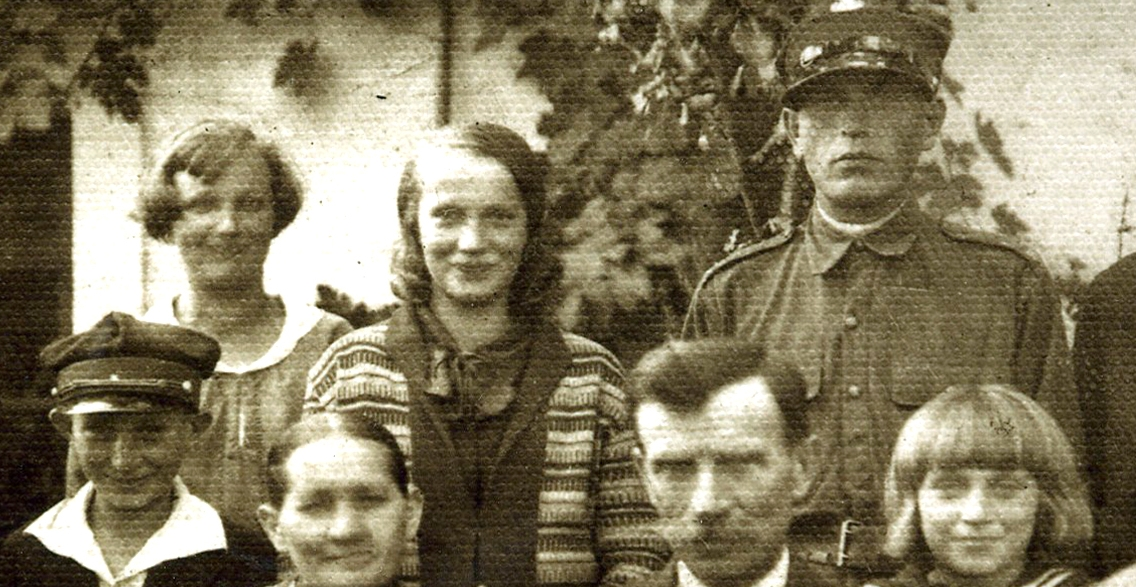
\includegraphics[width=0.65\textwidth]{photo/irena_swierczynska_1.jpg}
\caption[Irena Świerczyńska obok siostry Anastazji i brata Karola]{Irena Świerczyńska w drugim rzędzie (w środku) obok siostry Anastazji i brata Karola.}
\label{rys:irena_swierczynska_1}
\end{center}
\end{figure}

\begin{figure}[!h]
\begin{center}
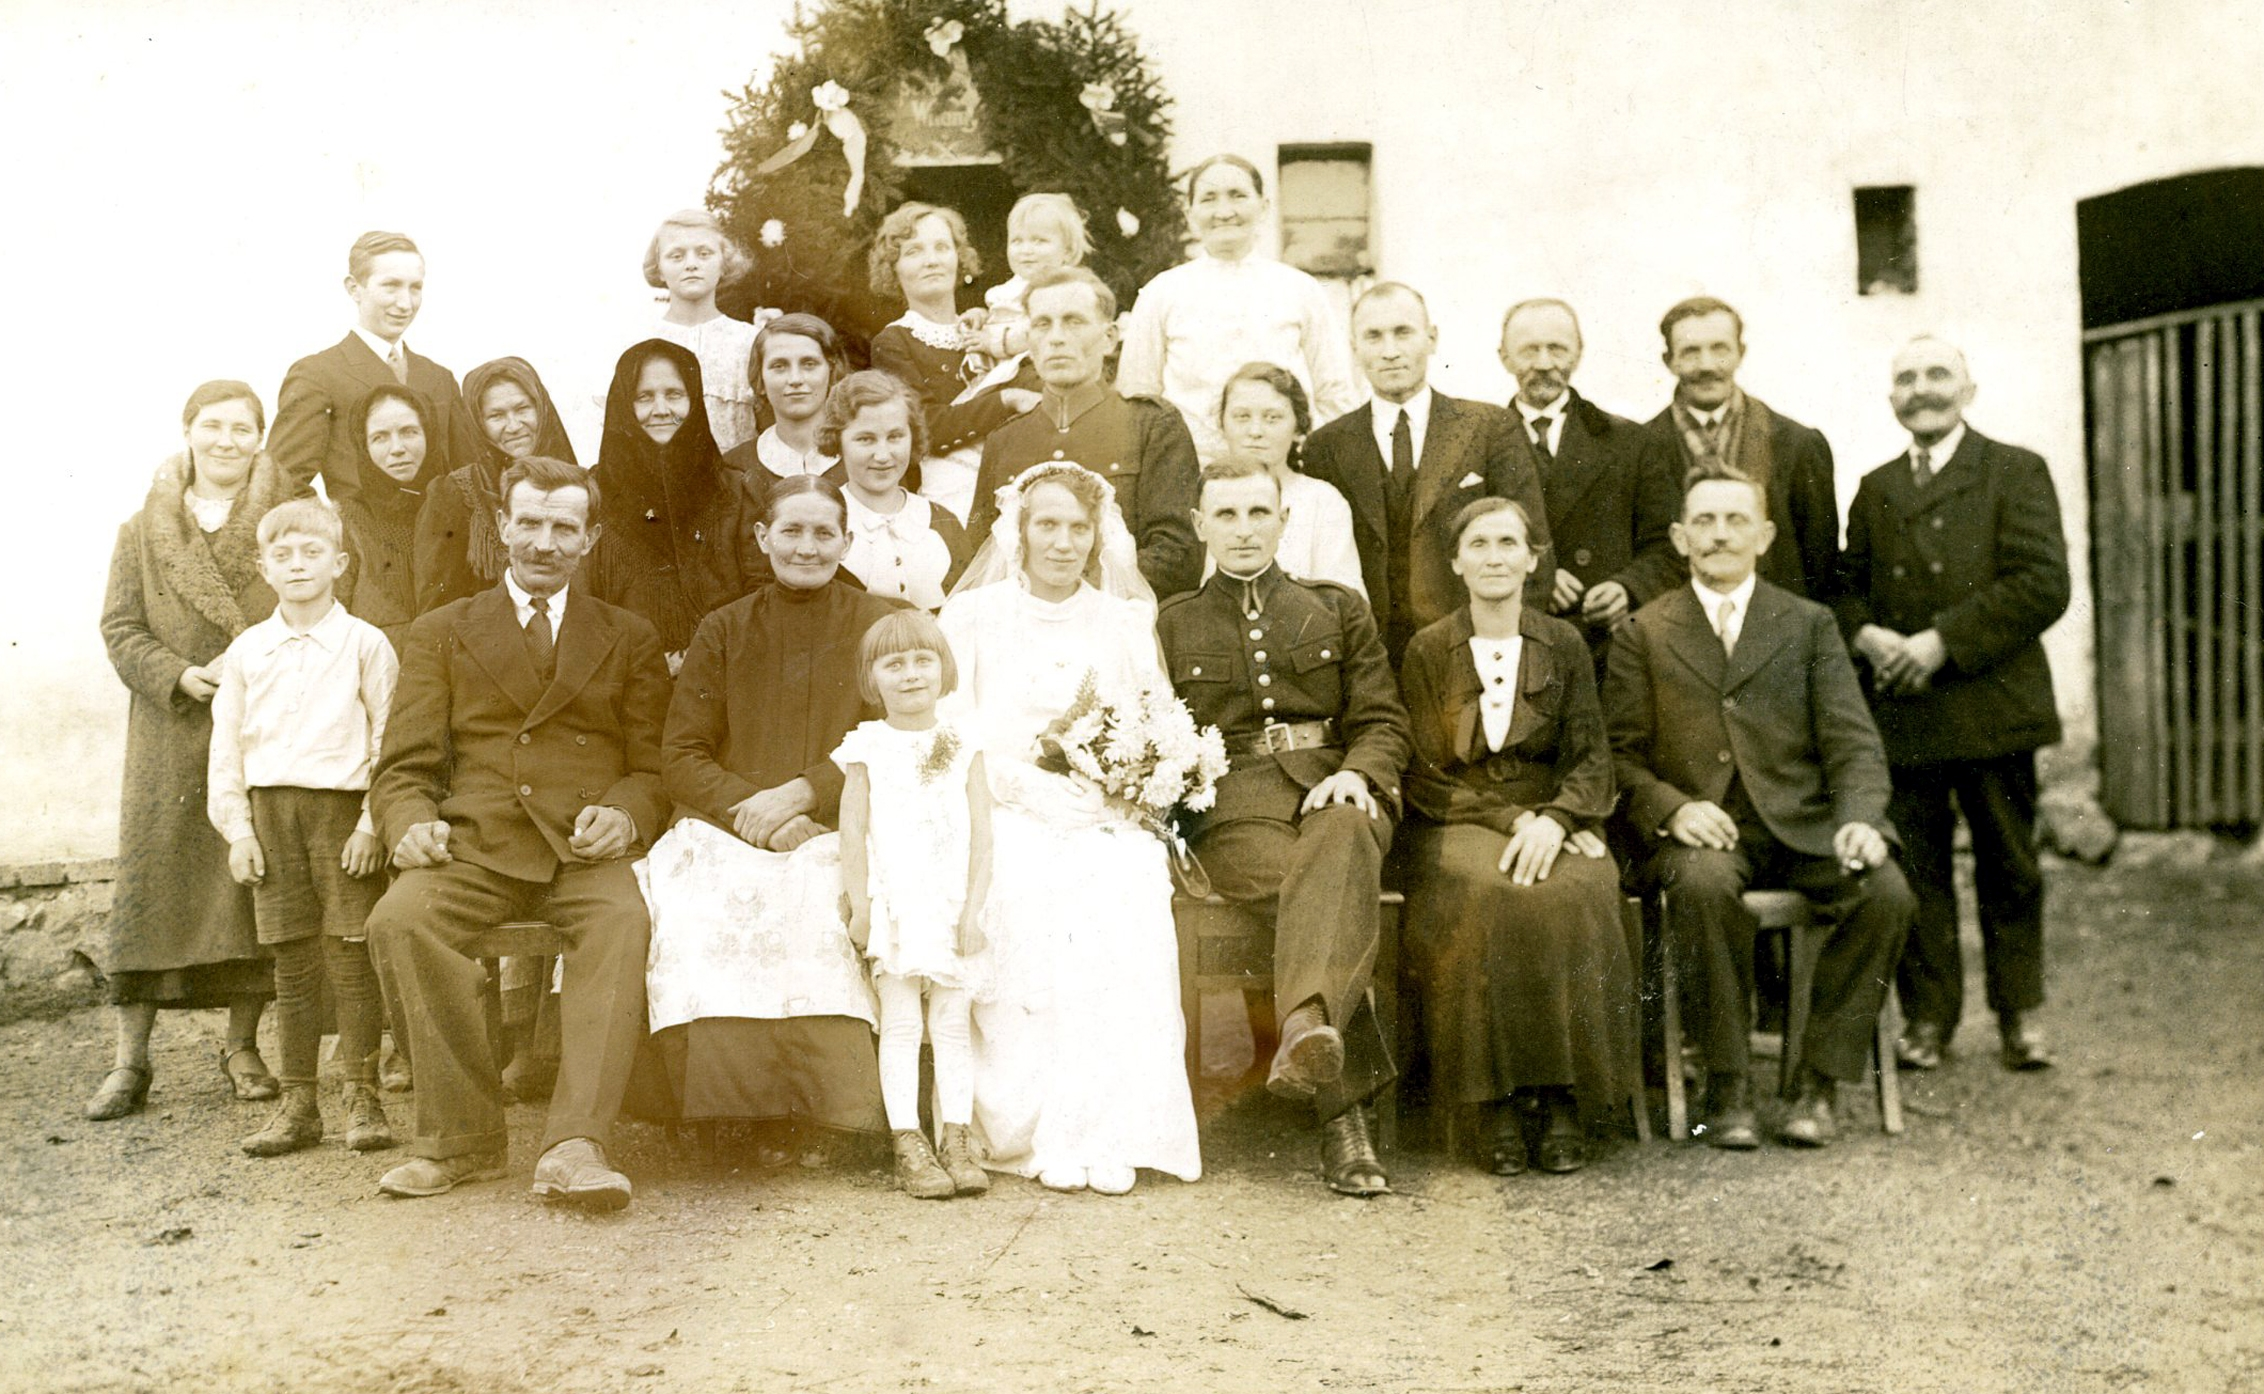
\includegraphics[width=0.93\textwidth]{photo/irena_antoni_lehman_slub.jpg}
\caption[Ślub Ireny i Antoniego Lehmanów]{Na zdjęciu siedzą od lewej: Edward Świerczyński z żoną Eufemią (z domu Grabińską), stoi przy babci Ela Świerczyńska, w środku Irena Świerczyńska Lehman i Antoni Lehman, obok siedzi jego matka Seweryna Lehman i Karol Grabiński (brat Eufemii). Stoją od lewej zaraz za siedzącymi: Paula Klimza, Eryk Grabiński (chłopiec), Elżbieta Berta Kuś, X. Kempa, Rózia Świerczyńska, Ela Janik (narzeczona stryja Karola) Karol Świerczyński, Bronia Grabińska, Leon Lehman, Y. Kempa, Furman weselny, Stary Klimza (sąsiad Świerczyńskich). W ostatnim rzędzie od lewej stoją: Benedykt Świerczyński, przy wieńcu stoi Eugenia Grabińska, u wejścia Ludwika Świerczyńska z rocznym Wirgusiem oraz Maria Wąs (z domu Grabińska, siostra babci Eufemii).}
\label{rys:irena_antoni_lehman_slub}
\end{center}
\end{figure}

Tam też ukończyła szkołę podstawową. Dzięki bratu Karolowi poznała o 10 lat starszego od siebie mężczyznę -- podobnie jak on -- strażnika więziennego -- \textbf{Antoniego Lehmana, za którego wyszła 7 listopada 1936~r. w Łagiewnikach Wielkich}.

Miała z nim czterech synów: \textbf{Tadeusza ur. 6 lutego 1938 r. w Łagiewnikach Wielkich, Lucjana ur. 2 marca 1941 r. w Łagiewnikach Wielkich, który zmarł wkrótce, bo już 19 kwietnia 1941 r. tamże, Gustawa ur. 7 lutego 1943 r. także w Łagiewnikach Wielkich oraz Bogumiła ur. 2 czerwca 1956 r. w Katowicach}.

\begin{figure}[!h]
\begin{center}
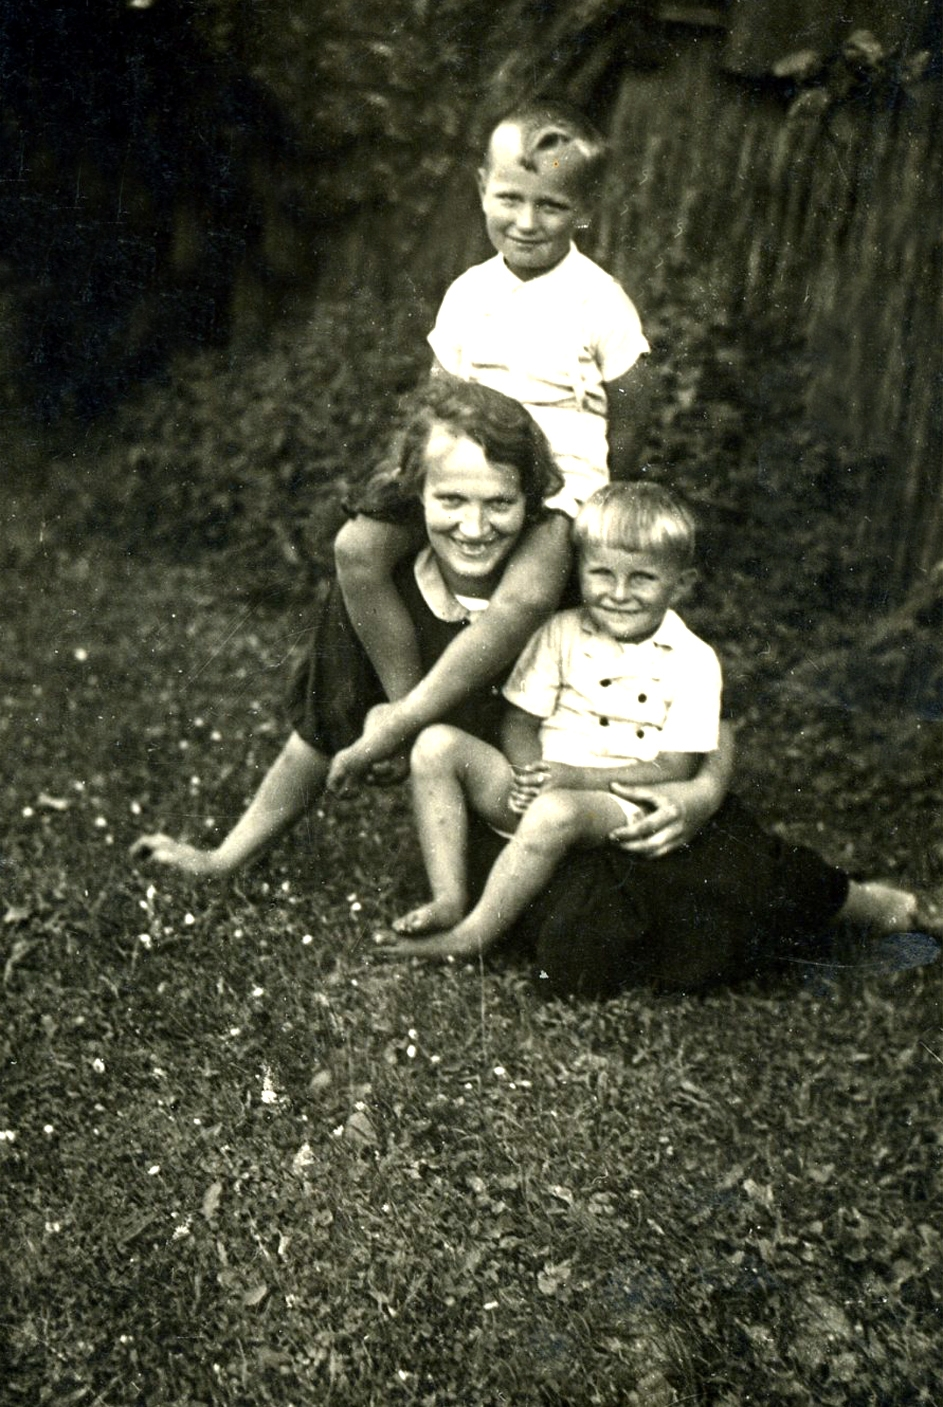
\includegraphics[width=0.32\textwidth]{photo/tadeuasz_lehman_1.jpg}
\caption[Tadeusz Lehman]{Tadeusz Lehman (na kolanach mamy Ireny), a na jej szyi siedzi Wirguś Świerczyński.}
\label{rys:tadeuasz_lehman_1}
\end{center}
\end{figure}

\begin{figure}[!h]
\begin{center}
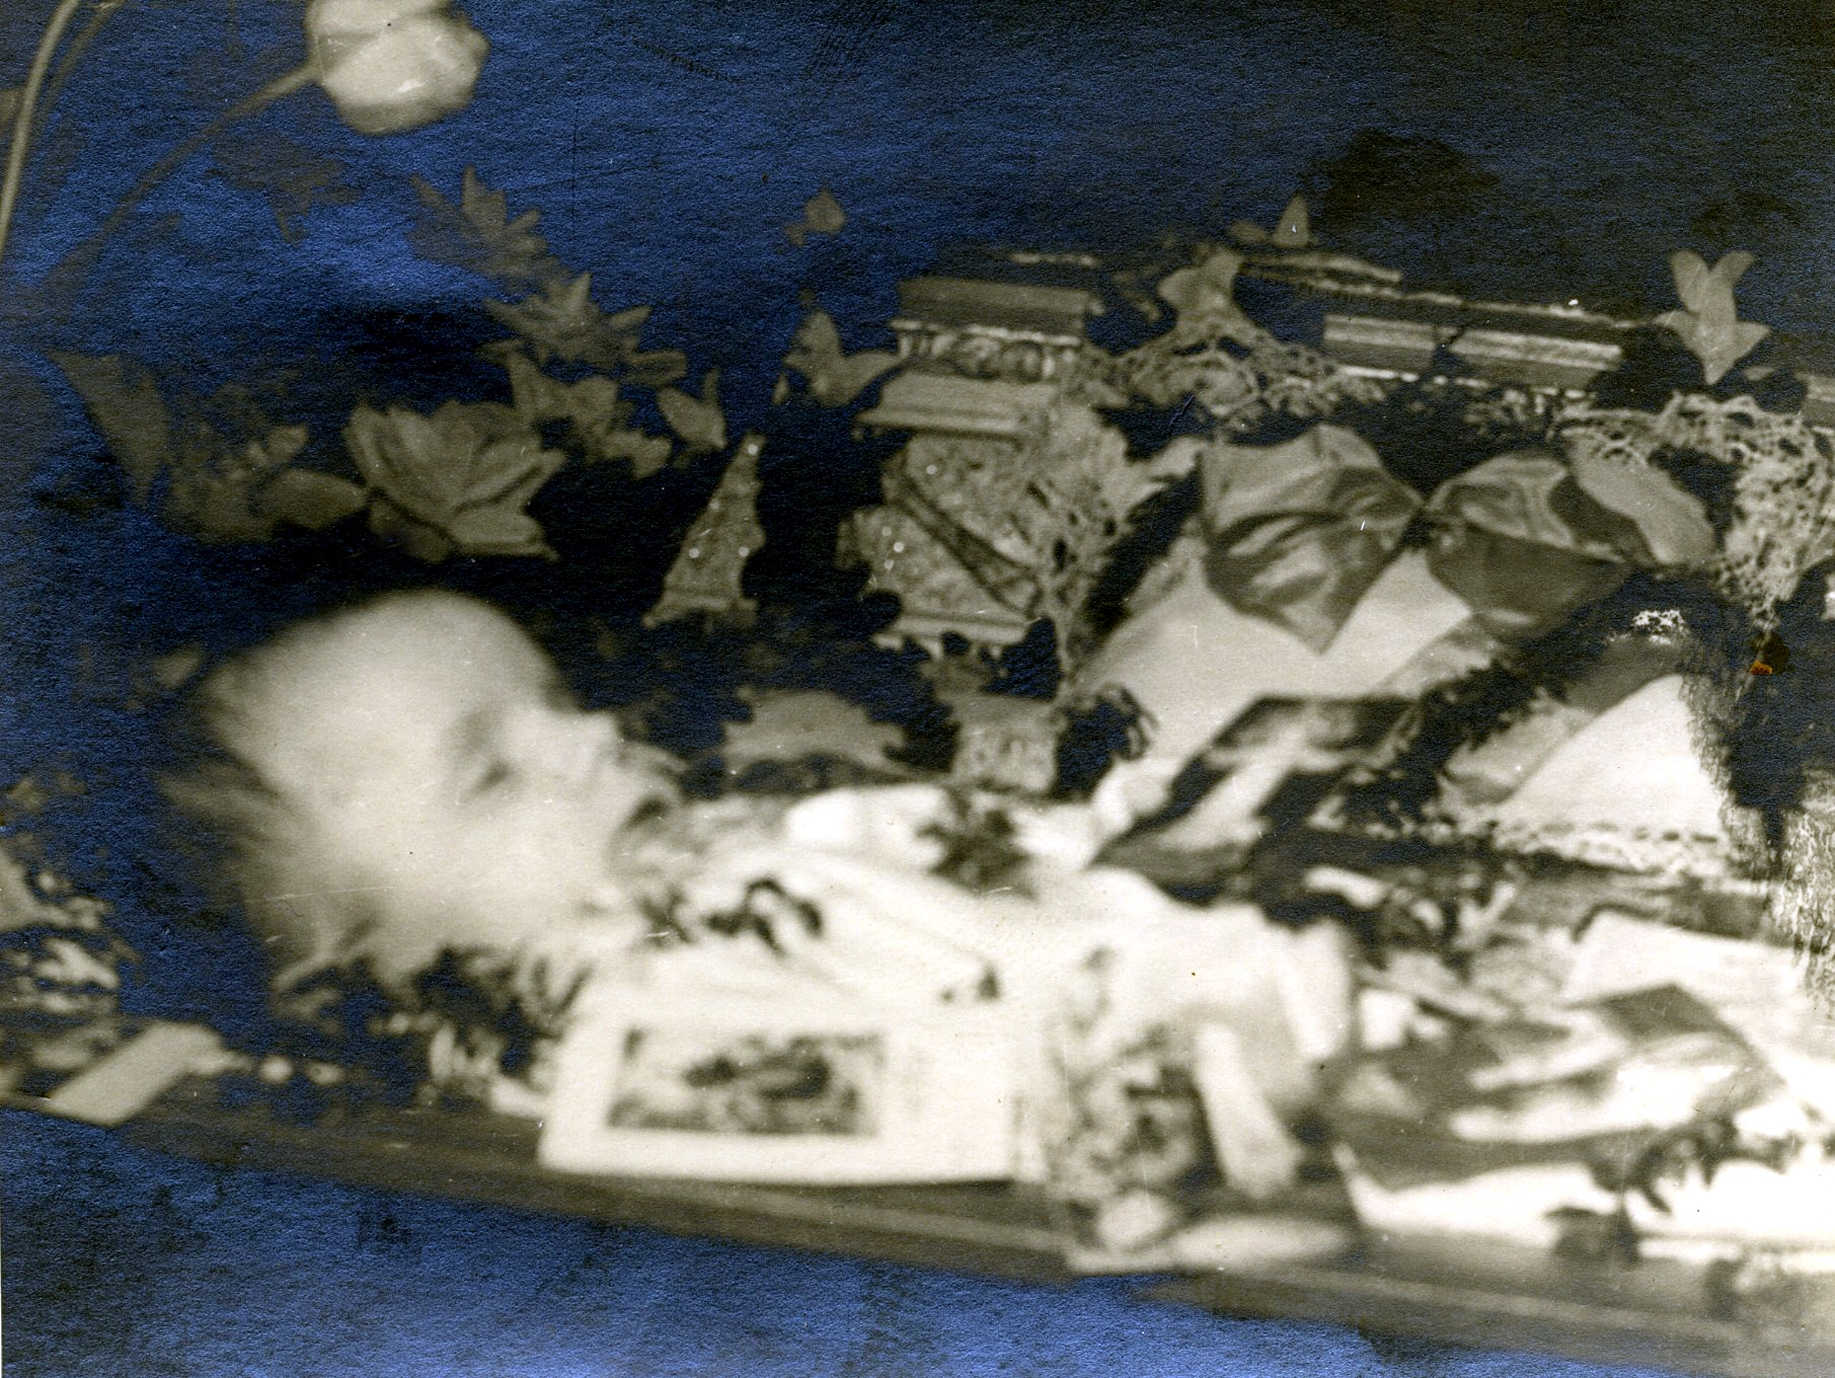
\includegraphics[width=0.4\textwidth]{photo/lucjan_lehman_w_trumience.jpg}
\caption{Lucjan Lehman w trumience}
\label{rys:lucjan_lehman_w_trumience}
\end{center}
\end{figure}

\begin{figure}[!h]
\begin{center}
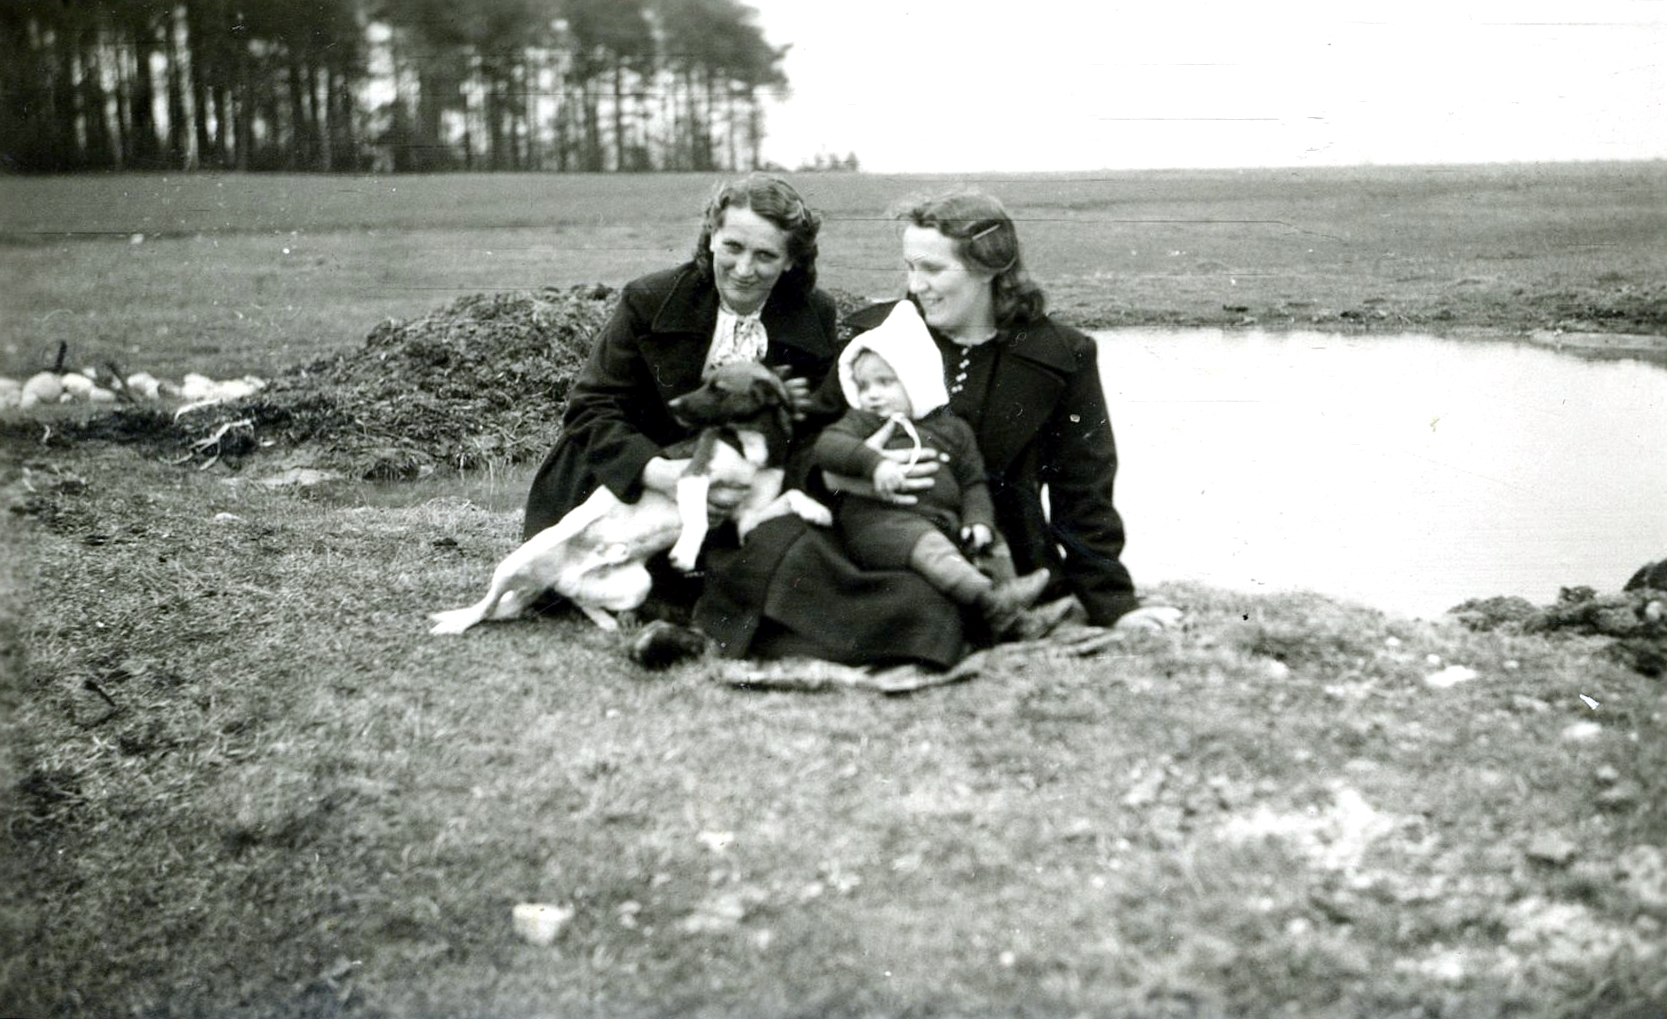
\includegraphics[width=0.5\textwidth]{photo/gustaw_lehman_1.jpg}
\caption[Gustaw Lehman]{Na zdj. Gustaw Lehman siedzi u mamy Ireny, obok Róża Świerczyńska z psem.}
\label{rys:gustaw_lehman_1}
\end{center}
\end{figure}

\begin{figure}[!h]
\begin{center}
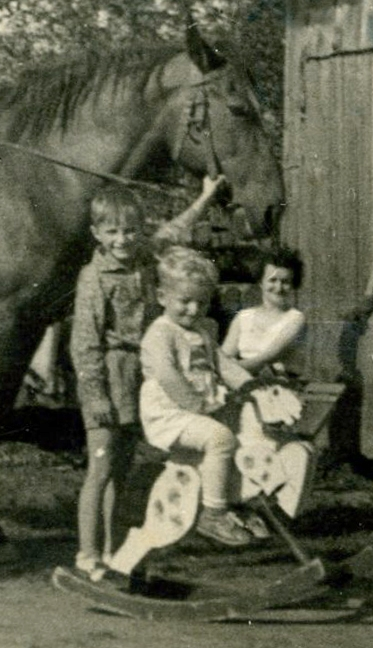
\includegraphics[width=0.3\textwidth]{photo/bogumil_lehman_1.jpg}
\caption[Bogumił Lehman]{Bogumił Lehman (trzymający konia za uzdę), przed nim na koniku bujanym Bogdan Kuś, obok siedzi babcia Radinka.}
\label{rys:bogumil_lehman_1}
\end{center}
\end{figure}

Pierwsze lata małżeństwa mieszkali przy naszych Dziadkach na Wieskach, później, gdy spodziewali się pierwszego potomka przenieśli się do mieszkania we dworze w Łagiewnikach Wielkich. Tam przyszedł na świat Tadeusz, później Lucjan, który wkrótce zmarł i Gustaw. Ten czas sielski – anielski trwał do przyjścia na świat Gustawa w 1943 r.

Stryj Antoni zostaje wysłany na front zachodni i tam jako żołnierz Wehrmachtu dostaje się do niewoli, skąd trafia do Wojska Polskiego we Francji. Służył w stopniu plutonowego w Awinionie, na południu Francji, w dawnej stolicy papieskiej, a następnie w Noyon w departamencie Oise -- na północ od Paryża, skąd w listopadzie 1945~r. wraca do Polski Ludowej. Tu czeka go wielkie rozczarowanie. Niejaki Sosnowski doniósł na niego w UB, że niby znęcał się nad więźniami ze względów ideowych, a przecież stryj Antoni był strażnikiem w więzieniu kryminalnym (nie politycznym) i ów Sosnowski siedział za złodziejstwo, skazany przez polski, przedwojenny sąd. Stryj ma nazwisko niemieckie, urodził się w Essen, służył w Wehrmachcie i był strażnikiem więziennym w znienawidzonej przez sowieckiego okupanta Polsce sanacyjnej. Czyż trzeba było wówczas więcej, by skazać człowieka na ciężkie więzienie a nawet śmierć?! Został aresztowany 10 kwietnia 1946~r. i wyrokiem Sądu Okręgowego w Bytomiu z dnia 14 kwietnia 1947 r. skazany na 8 lat więzienia, którą to karę odbył w więzieniu w Sztumie (na południe od Malborka). Wyszedł z więzienia na podstawie amnestii (po śmierci Stalina). W więzieniu pracował w warsztacie samochodowym.

\begin{figure}[!h]
\begin{center}
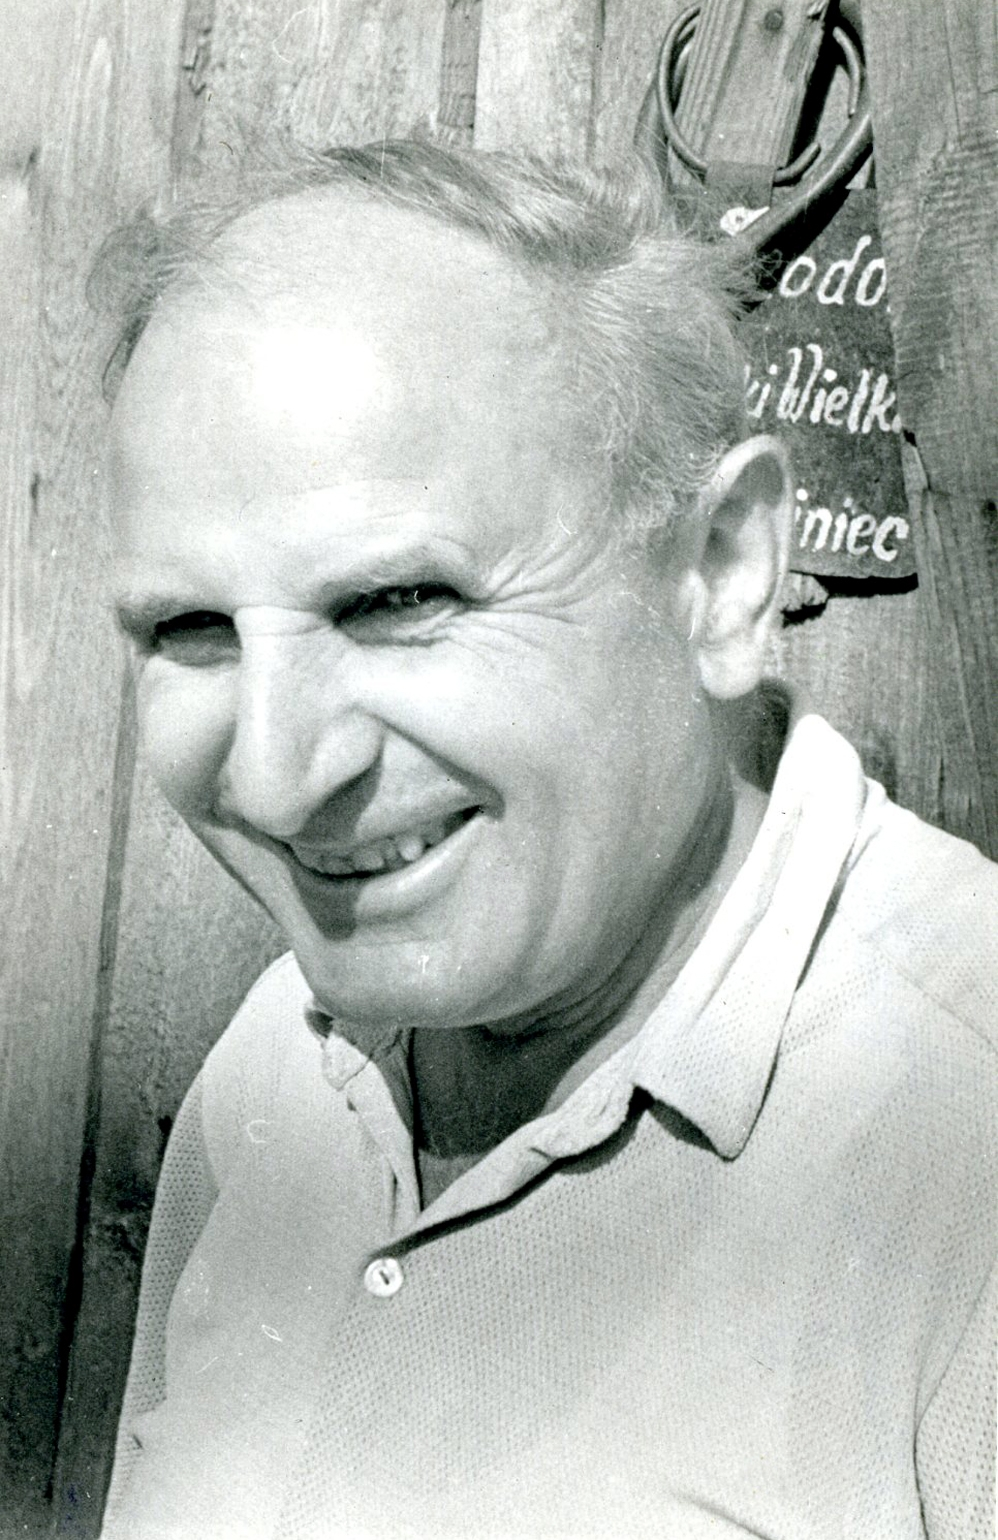
\includegraphics[width=0.3\textwidth]{photo/antoni_lehman_1.jpg}
\caption{Antoni Lehman}
\label{rys:antoni_lehman_1}
\end{center}
\end{figure}

Stryjenka Irena, chcąc ratować męża przed niesłusznym więzieniem, wybrała się z naszym Tatą do wsi Kuleje, by szukać tam świadków niewinności swego męża. I gdzieś w tych okolicach natknęli się na partyzantkę antysowiecką -- Narodowych Sił Zbrojnych, a nasz Tata był oficerem Ludowego Wojska Polskiego i jeszcze pracownikiem Urzędu Wojewódzkiego w Katowicach. Był więc w oczach tych ludzi -- niewątpliwych patriotów -- pachołkiem Rosji Sowieckiej. Chcieli go ,,rozwalić'', tam w lesie, lecz stryjenka Irena powiedziała im, że bez brata nigdzie się nie ruszy. Jej odwaga uratowała życie naszemu Tacie… Puścili ich razem wolno. Piękny przykład miłości siostrzanej i… braterskiej (bo narażał się nasz Ojciec dla męża swej siostry i w końcu utracił intratną posadę w Urzędzie Wojewódzkim, gdyż zdaniem swych przełożonych bronił Niemca, za jakiego w ich oczach uchodził stryj Antoni!).

\begin{figure}[!h]
\begin{center}
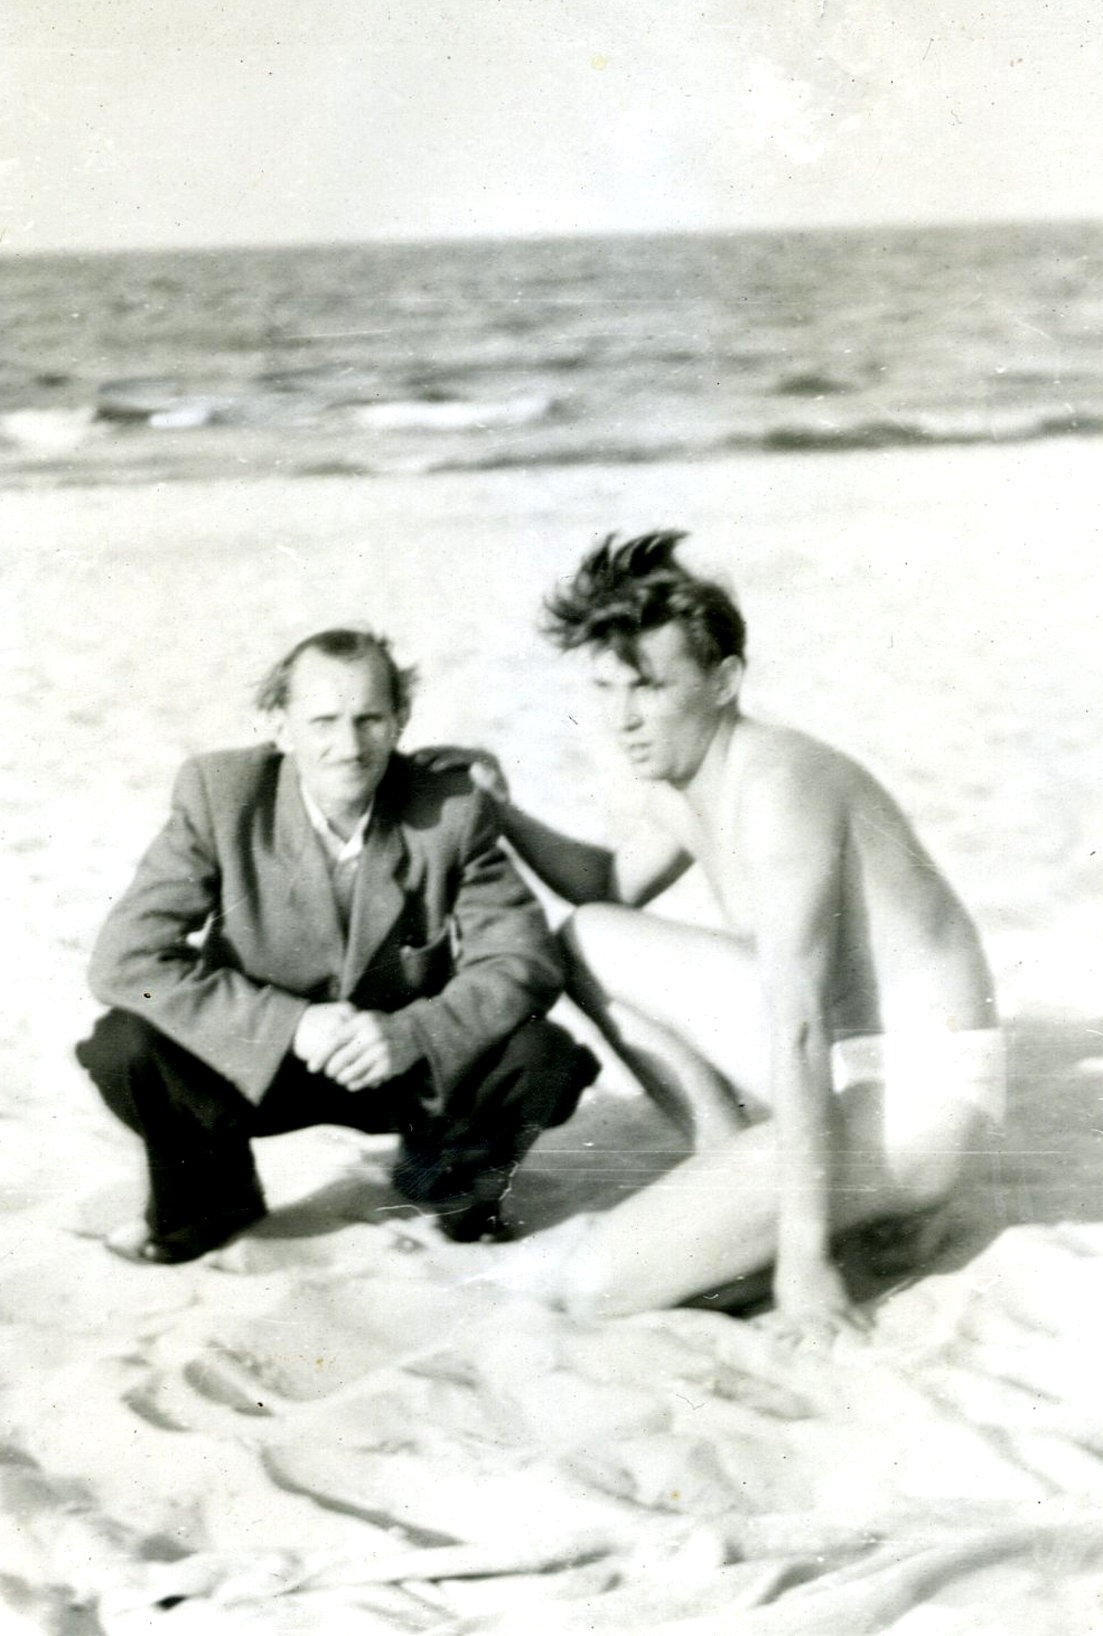
\includegraphics[width=0.3\textwidth]{photo/andrzej_lehman.jpg}
\caption[Andrzej Lehman]{Na zdj. Andrzej Lehman, brat Antoniego, z jego synem - Tadeuszem.}
\label{rys:andrzej_lehman}
\end{center}
\end{figure}

Stryjenka Irena, by być bliżej swego męża przyjęła z zadowoleniem nakaz pracy w Klinice Akademickiej w Gdańsku Wrzeszczu -- zaraz po ukończeniu Państwowej Szkoły Położnych w Chorzowie. Kwestię mieszkania najpierw pomogła jej rozwiązać rodzina Andrzeja Lehmana -- brata Antoniego, a następnie rodzona siostra Anastazja Świerczyńska, w zakonie Aurelia – siostra dla swej siostry zakonnej Celiny. Owa siostra Celina poprosiła swoją siostrę -- Klarę Miodek -- zamieszkałą w Gdańsku Wrzeszczu przy ul. Dzielnej 21 -- by mogła u niej mieszkać stryjenka Irena. I tak się stało. Mieszkała u niej do czasu wyjścia stryja Antoniego z więzienia w Sztumie.

Gdy stryj Antoni dostał pracę w Przedsiębiorstwie Transportowo -- Spedycyjnym Budownictwa Węglowego w Katowicach -- Załężu zamieszkali najpierw u Stryja Józefa w Katowicach Ligocie, a następnie od 1954 r. w Tychach, w bloku przy ul Bieruta 39/25, gdzie otrzymali mieszkanie. Tam z nimi zamieszkała matka stryja Antoniego -- Seweryna Lehman.

\begin{figure}[!h]
\begin{center}
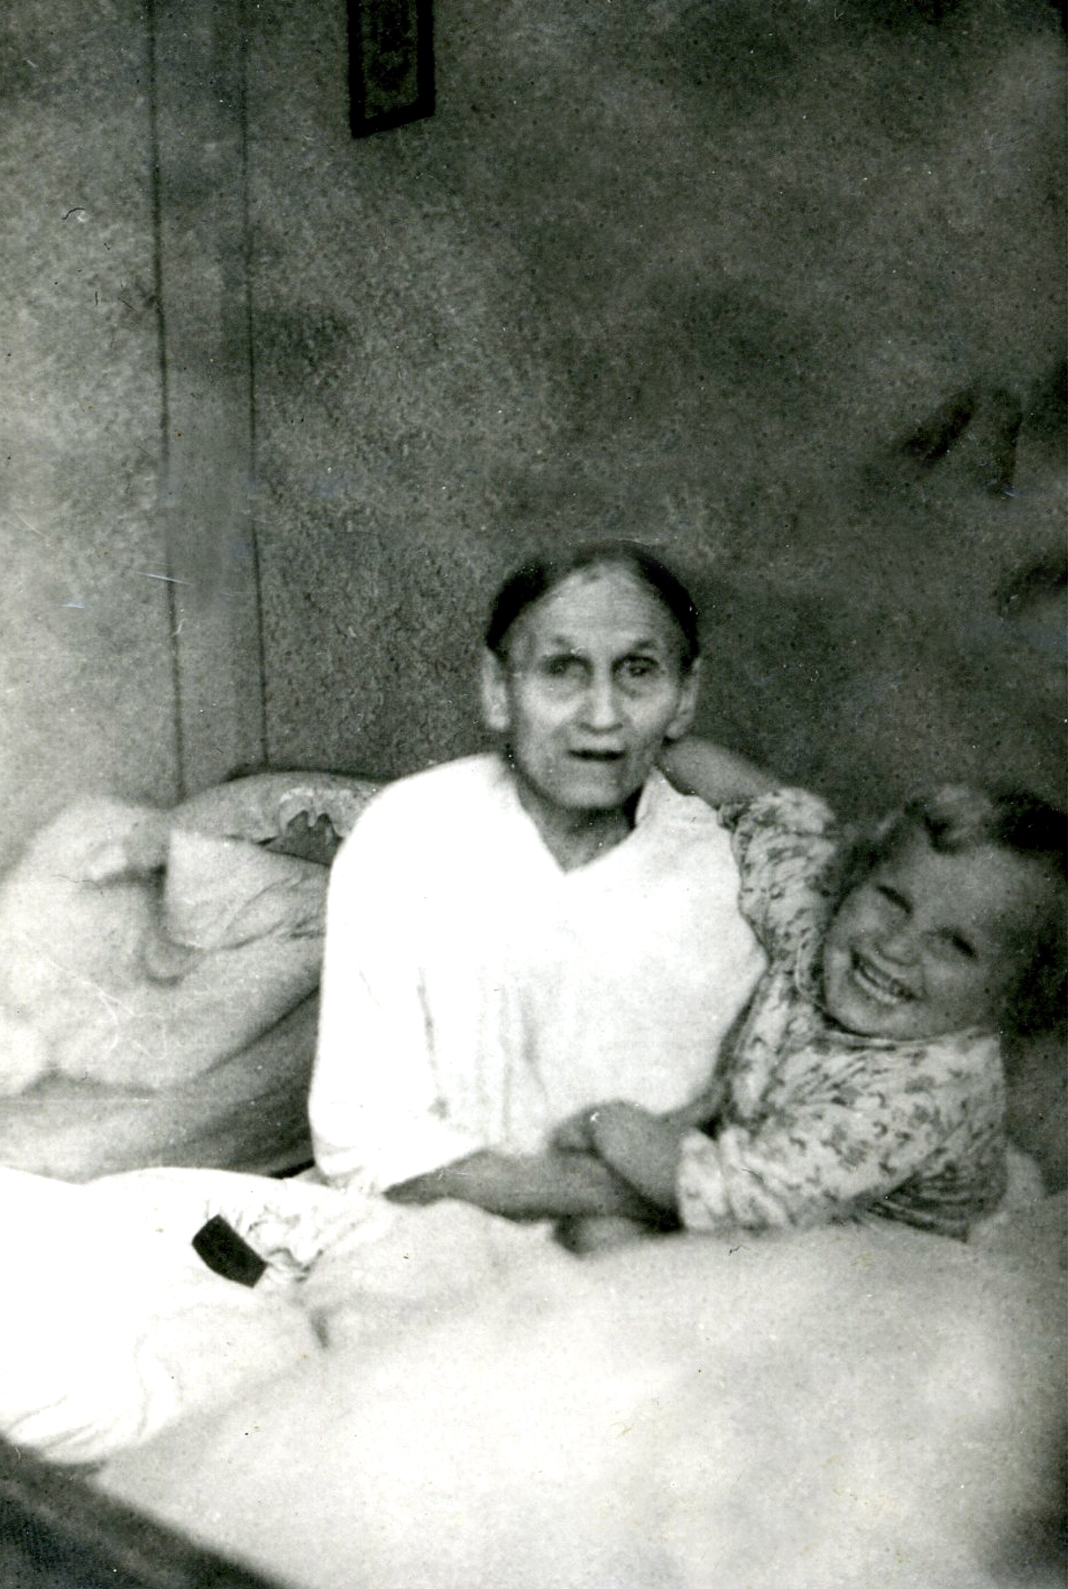
\includegraphics[width=0.3\textwidth]{photo/seweryna_lehman.jpg}
\caption[Seweryna Lehman z wnukiem Bogusiem]{Na zdj. Seweryna Lehman, matka Antoniego, z wnukiem Bogusiem.}
\label{rys:seweryna_lehman}
\end{center}
\end{figure}

Wkrótce też dołączył do nich \textbf{Bogumił, który przyszedł na świat 2 czerwca 1956 r.} w Szpitalu Im. Ludwika Rydygiera w Katowicach -- Bogucicach, gdzie pracowała jako położna jego mama -- stryjenka Irena i gdzie przyszła na świat Zuzia Świerczyńska oraz jej dwie córeczki -- Małgosia i Ania Kordusówne. Tam zresztą przyszła na świat większość jej wnuków i prawnuków. Szczęśliwy szpital dla naszej rodziny, który ma za patrona znakomitego lekarza chirurga, profesora Uniwersytetu Jagiellońskiego i Lwowskiego i jednocześnie wielkiego patriotę, który jako gen. bryg. brał udział w obronie Lwowa w 1918~r. i na własne życzenie został w 1920 r. pochowany na Cmentarzu Orląt Lwowskich.

\begin{figure}[!h]
\begin{center}
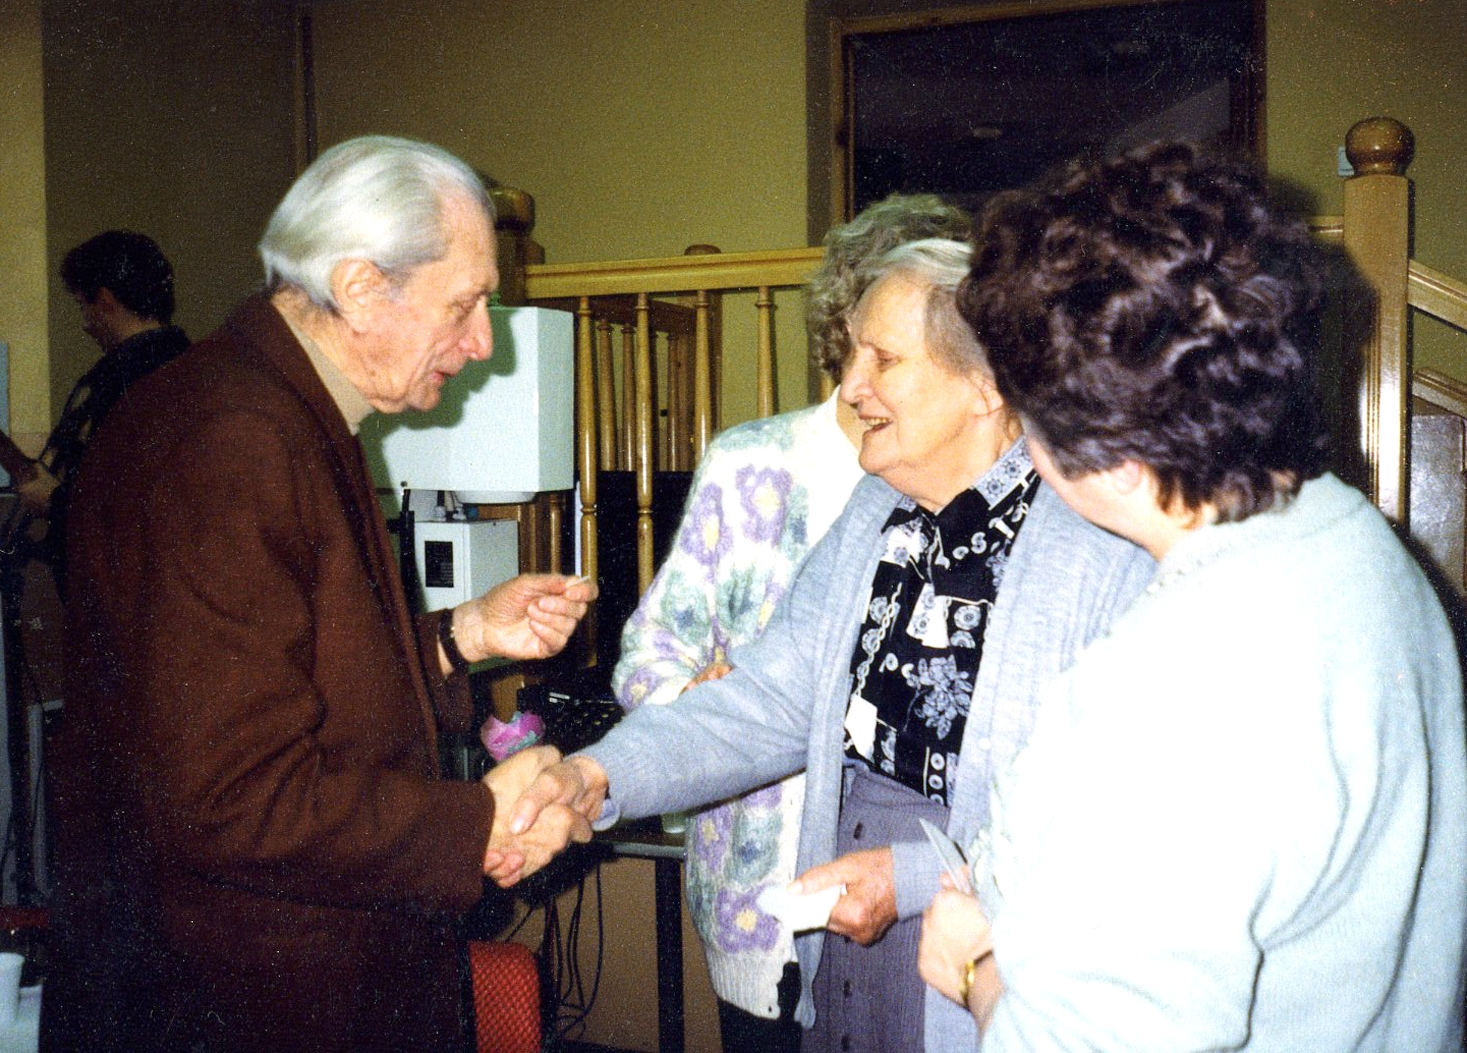
\includegraphics[width=0.7\textwidth]{photo/irena_lehman_1.jpg}
\caption{Irena Lehman przyjmuje od dra Skrzelewskiego, ordynatora Oddziału życzenia.}
\label{rys:irena_lehman_1}
\end{center}
\end{figure}

Gdy ów \textbf{Bogumił} miał dwa latka, a babcia Seweryna Lehman wyszła na miasto po sprawunki, zostawiając go pod opieką jego sześcioletniej kuzynki -- \textbf{Marysi Kusiównej} -- ten ze stołu w kuchni otwarł okno i\ldots z drugiego piętra wyszedł sobie na dwór, więc nagle znalazł się w pryzmie piasku! Złamał tylko piętę.\ldots \textbf{13 marca 1960 r. zmarła w wieku 76 lat babcia Ksawera (Seweryna) Lehman -- z domu Lubczyńska}, matka stryja Antoniego, która mieszkała u nich od 1955 r.

\begin{figure}[!h]
\begin{center}
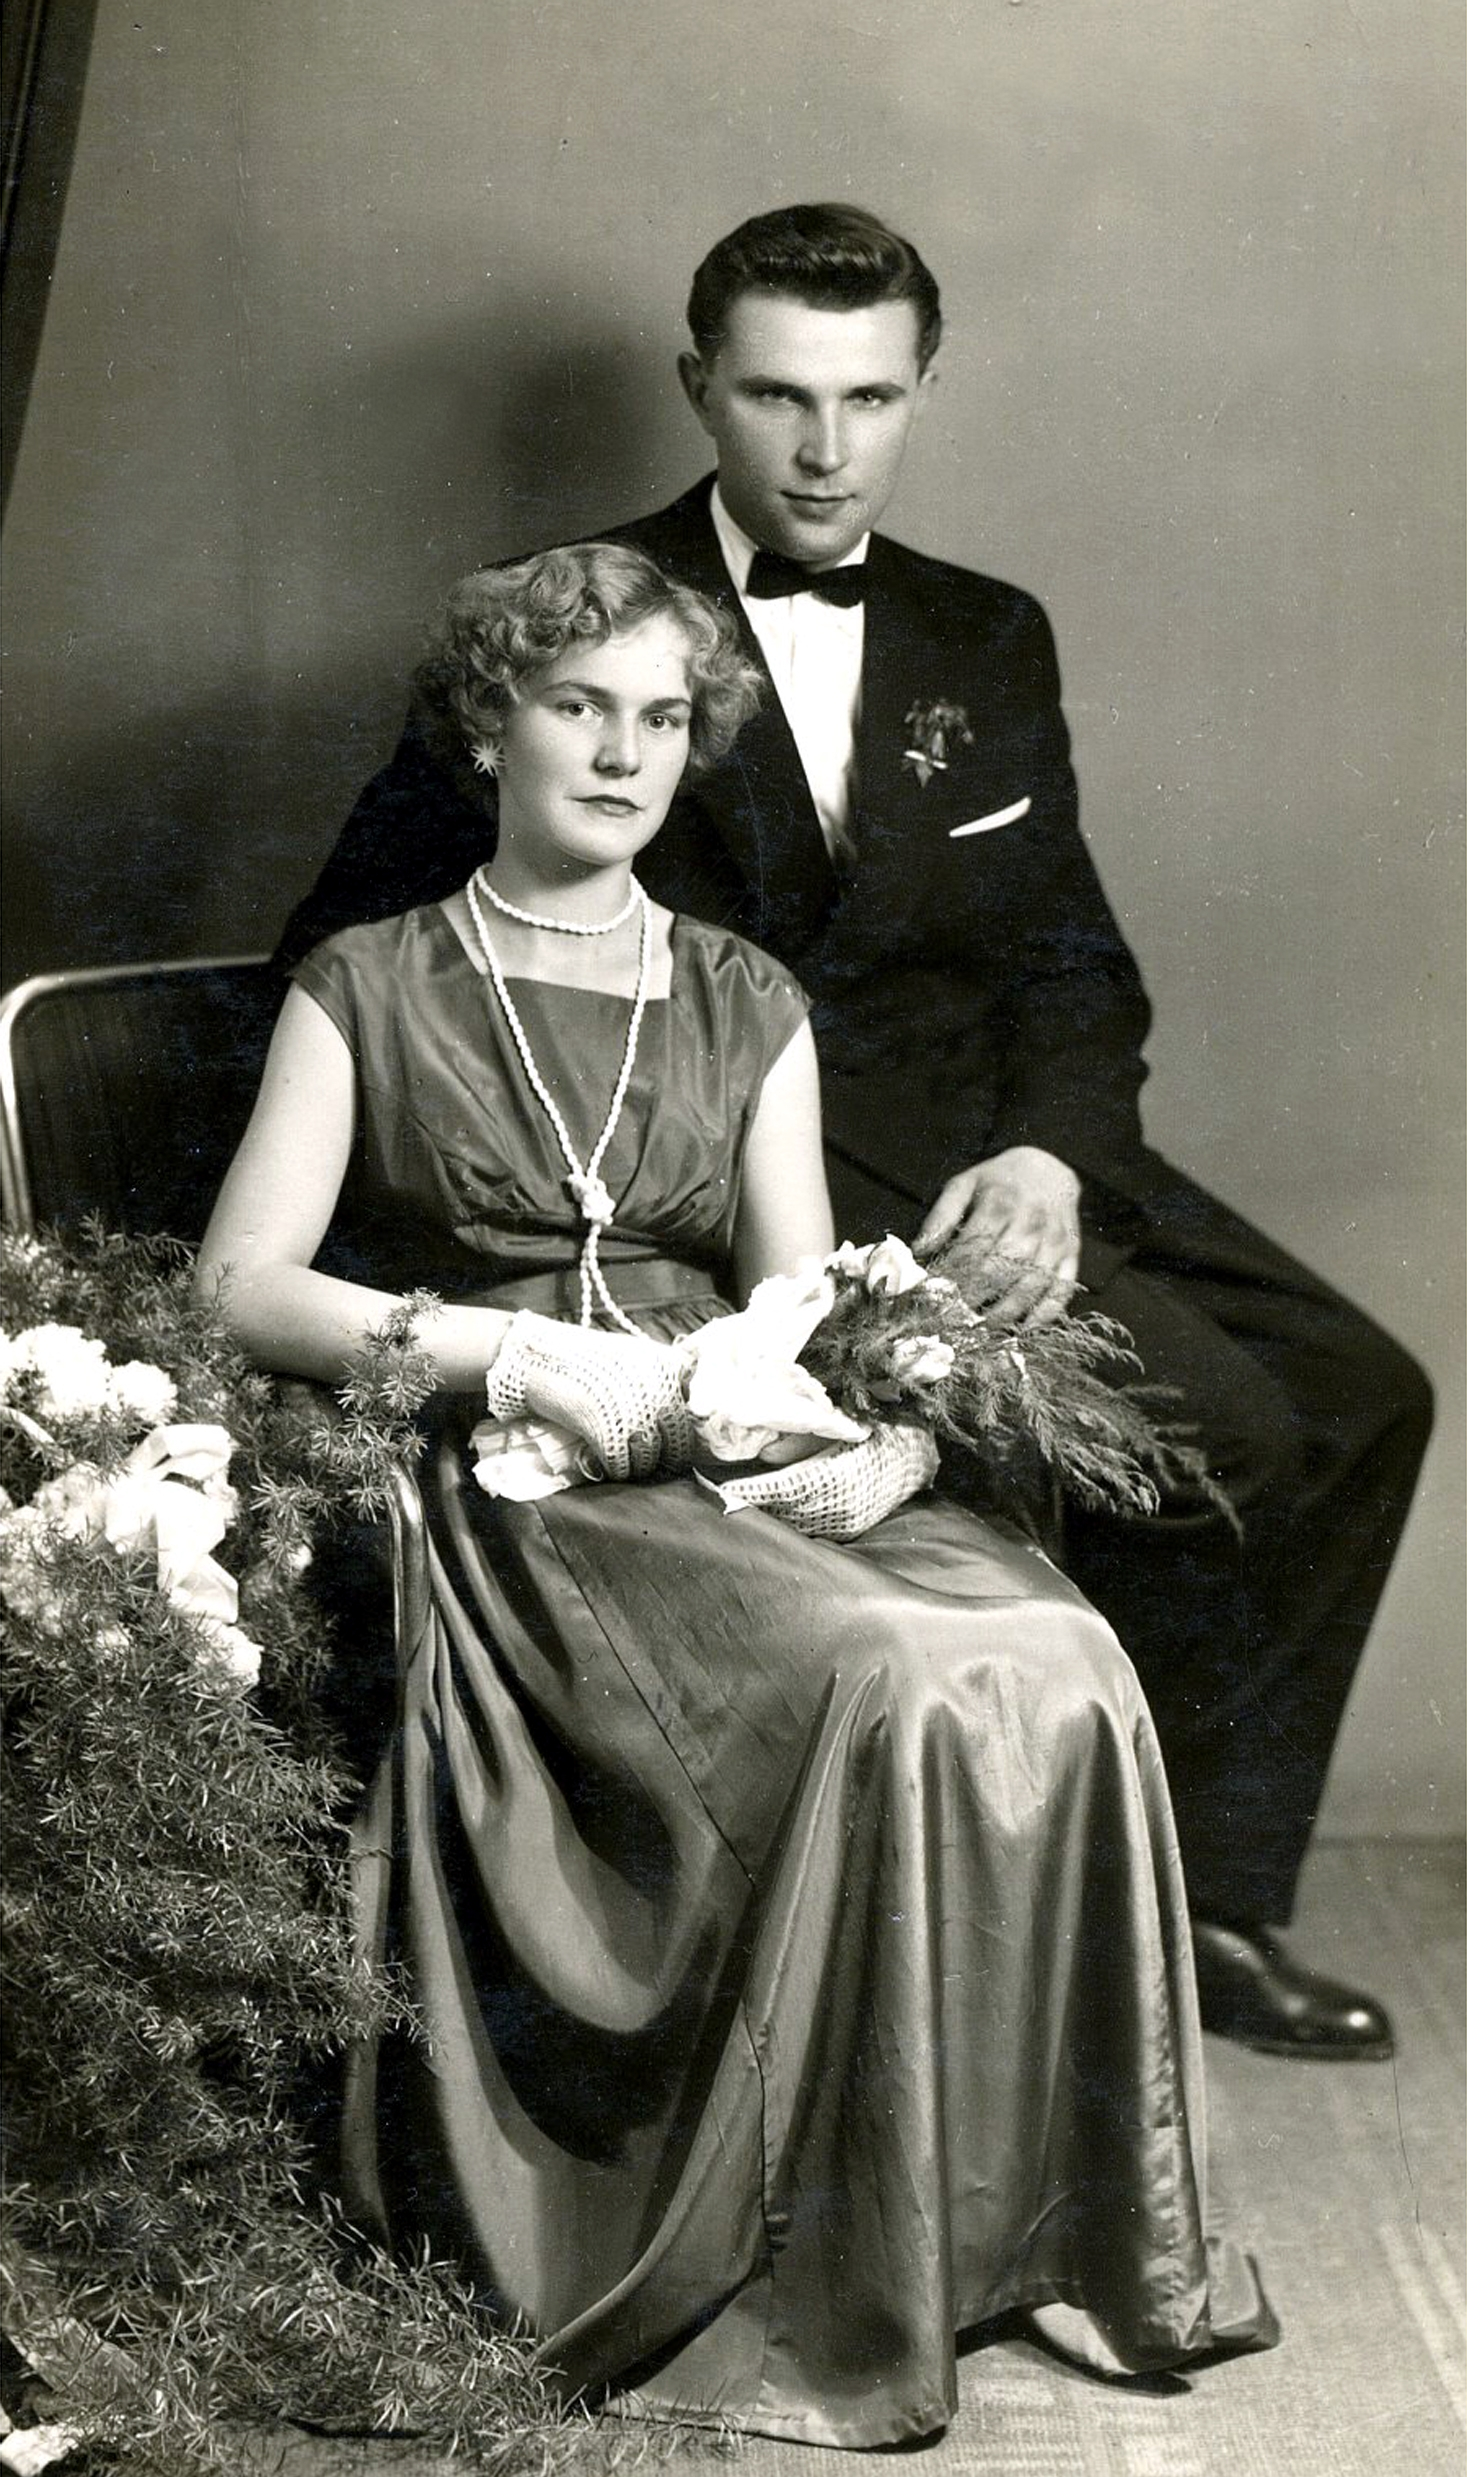
\includegraphics[height=75mm]{photo/tadeusz_lubomira_lehman_slub_1.jpg}
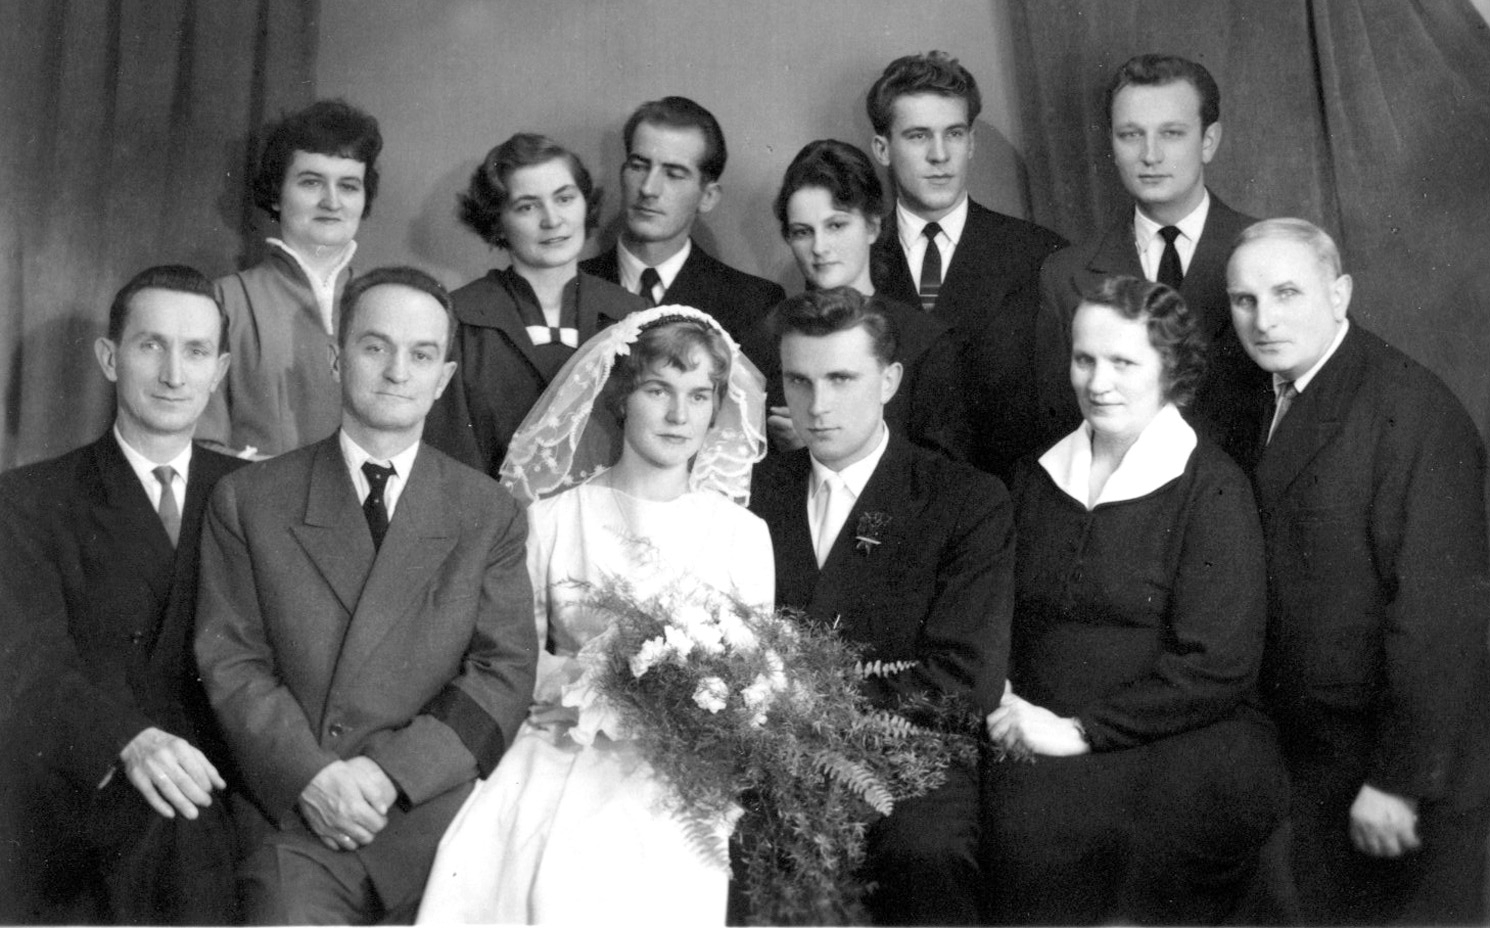
\includegraphics[height=75mm]{photo/tadeusz_lubomira_lehman_slub_2.jpg}
\caption[Ślub Lubomiry Szafron i Tadeusza Lehmana]{Ślub Lubomiry Szafron i Tadeusza Lehmana. Na zdj. zbiorowym od lewej: Radegunda i Benedykt Świerczyńscy, Konrad Szafron, Lubomira Szafron, Tadeusz Lehman, Irena i Antoni Lehmanowie, za nimi Wirgiliusz Świerczyński.}
\label{rys:tadeusz_lubomira_lehman_slub}
\end{center}
\end{figure}

Ich najstarszy syn -- Tadeusz około 1952 r. ukończył szkołę podstawową i trafił do Technikum Samochodowego w Gliwicach, gdzie uzyskał maturę i tytuł technika. W 1969 r. ukończył studia wyższe na Politechnice Gliwickiej, na Wydziale Spawalnictwa. \textbf{Tadeusz ożenił się 20 listopada 1960 r. z Lubomirą Szafron, córką Konrada i Marii z domu Potyka – urodzoną 26 czerwca 1936 r. w Ćwiklicach.}

Karierę zawodową rozpoczął w Tychach -- w Przedsiębiorstwie Transportowo Spedycyjnym. Potem przeniósł się do Pszczyny, do Przedsiębiorstwa Geologicznego, gdzie był szefem bazy. Wreszcie osiadł na dobre w PKS-ie w Pszczynie, gdzie od 1974 r. był dyrektorem dopóty, dopóki go białaczka nie wyeliminowała najpierw spośród pracujących, \textbf{a 25 lutego 2002r. spośród żyjących}.

\begin{figure}[!h]
\begin{center}
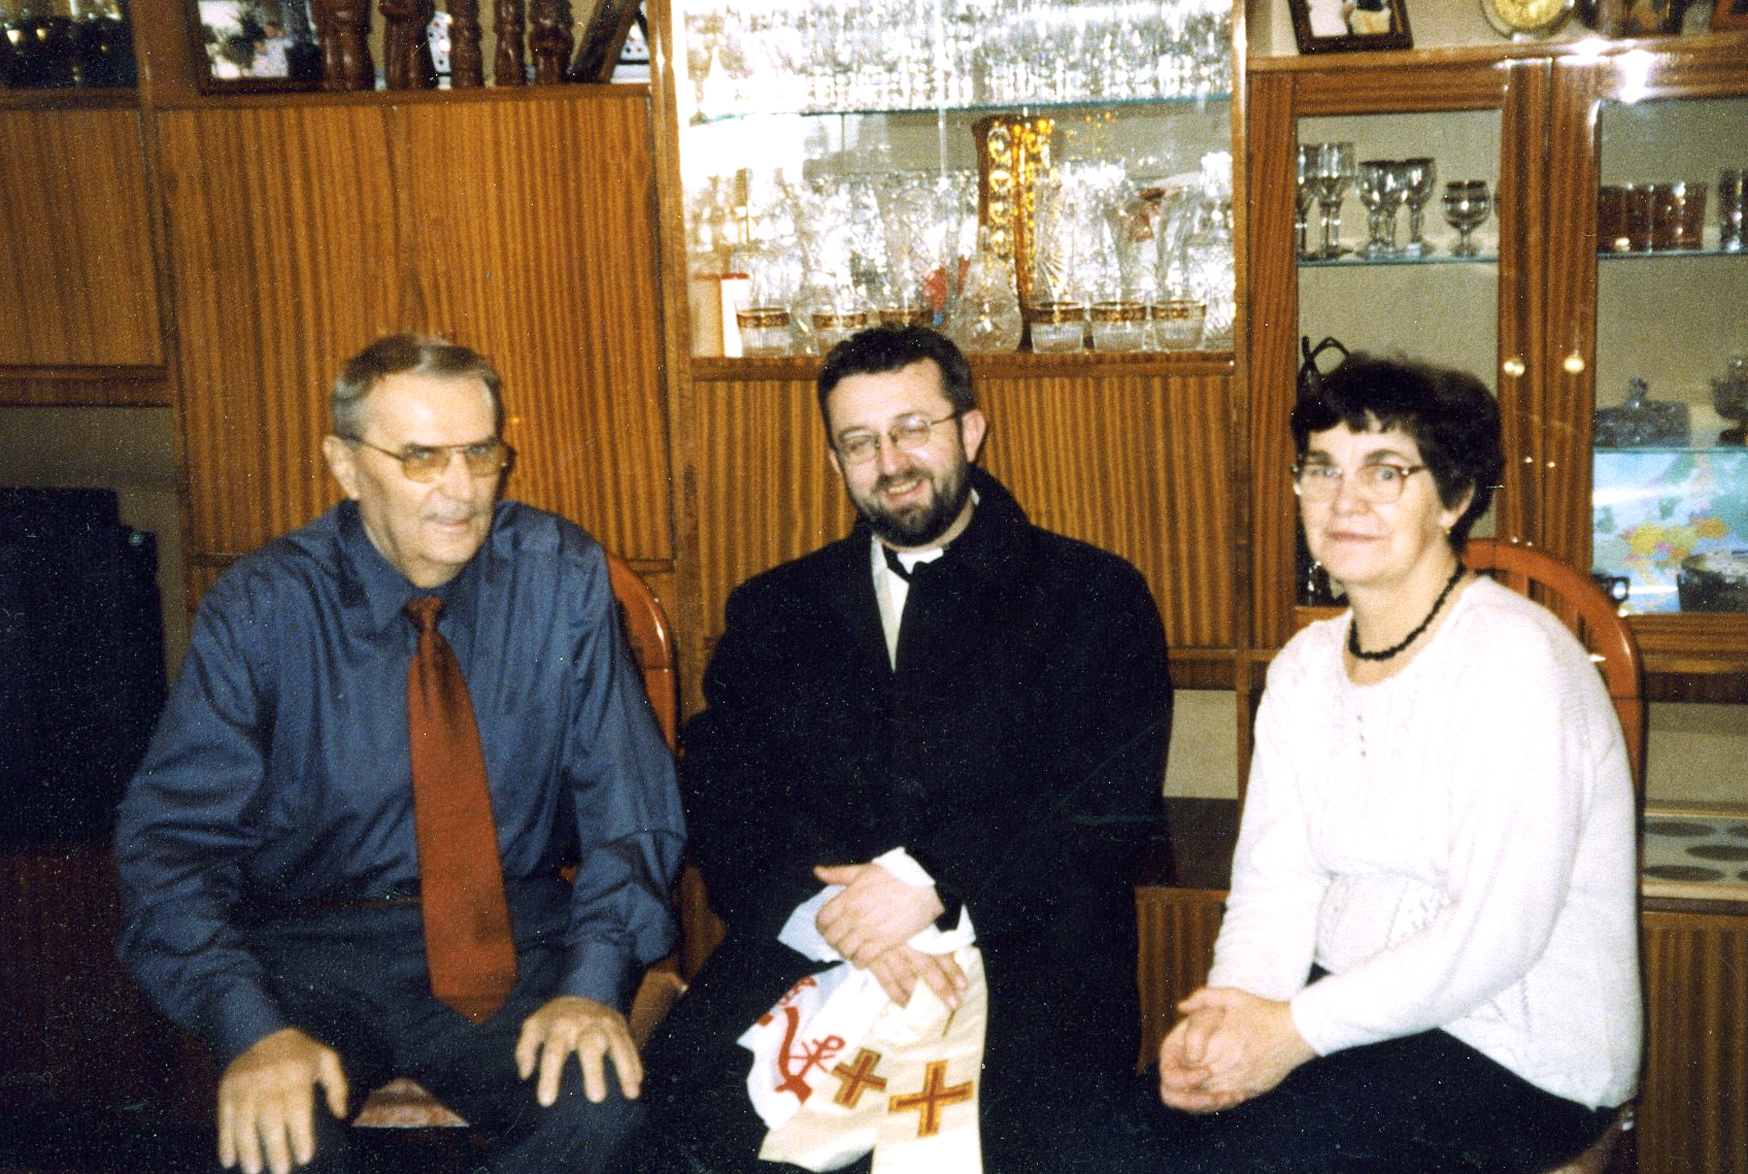
\includegraphics[width=0.6\textwidth]{photo/tadeusz_lubomira_lehman_1.jpg}
\caption{Lubomira i Tadeusz Lehmanowie z księdzem w 2002 r.}
\label{rys:tadeusz_lubomira_lehman_1}
\end{center}
\end{figure}

Lubomira ukończyła Technikum Budowlane i pracowała do emerytury w Wojewódzkim Przedsiębiorstwie GOP Południe w Tychach. Dochowali się czterech wspaniałych synów: \textbf{Grzegorza ur. 11 maja 1961 r. w Ćwiklicach, Andrzeja ur. 30 listopada 1964 r. w Katowicach} (on i następni w Szpitalu Im. Ludwika Rydygiera u babki Lehmanki), \textbf{Krzysztofa ur. 21 kwietnia 1972 r. i Tomasza ur. 4 grudnia 1973~r}.

\begin{figure}[!h]
\begin{center}
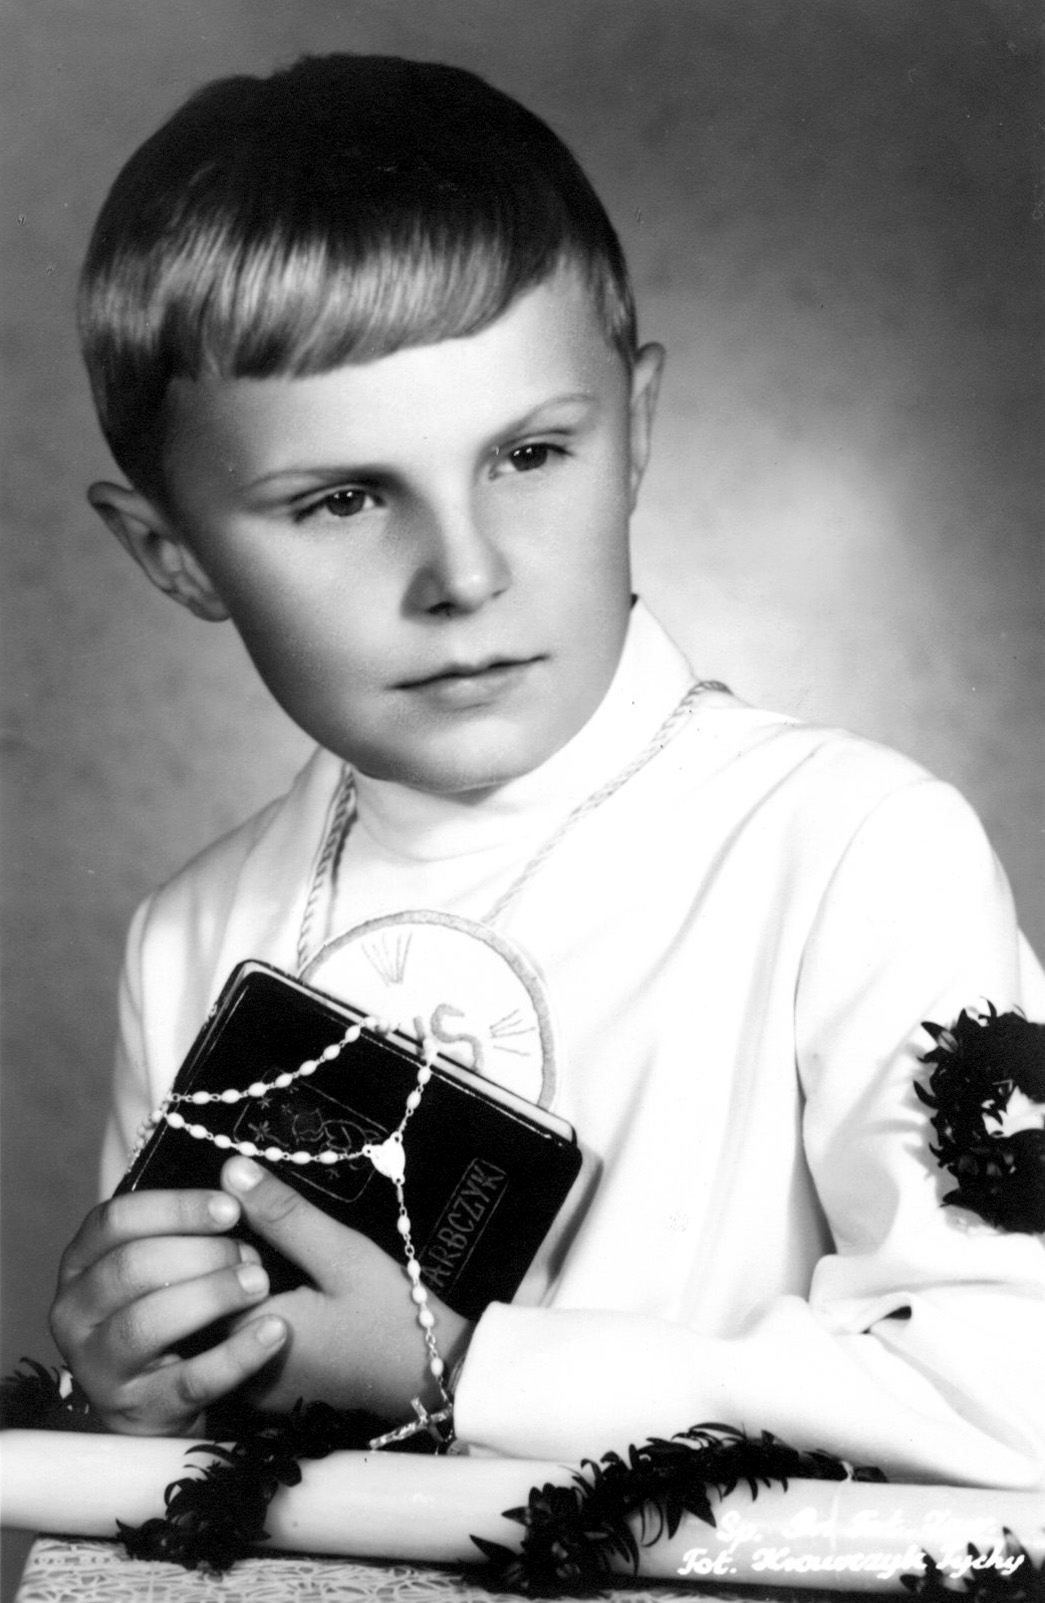
\includegraphics[width=0.3\textwidth]{photo/grzegorz_lehman.jpg}
\caption{Grzegorz Lehman u I Komunii św.}
\label{rys:grzegorz_lehman}
\end{center}
\end{figure}

\begin{figure}[!h]
\begin{center}
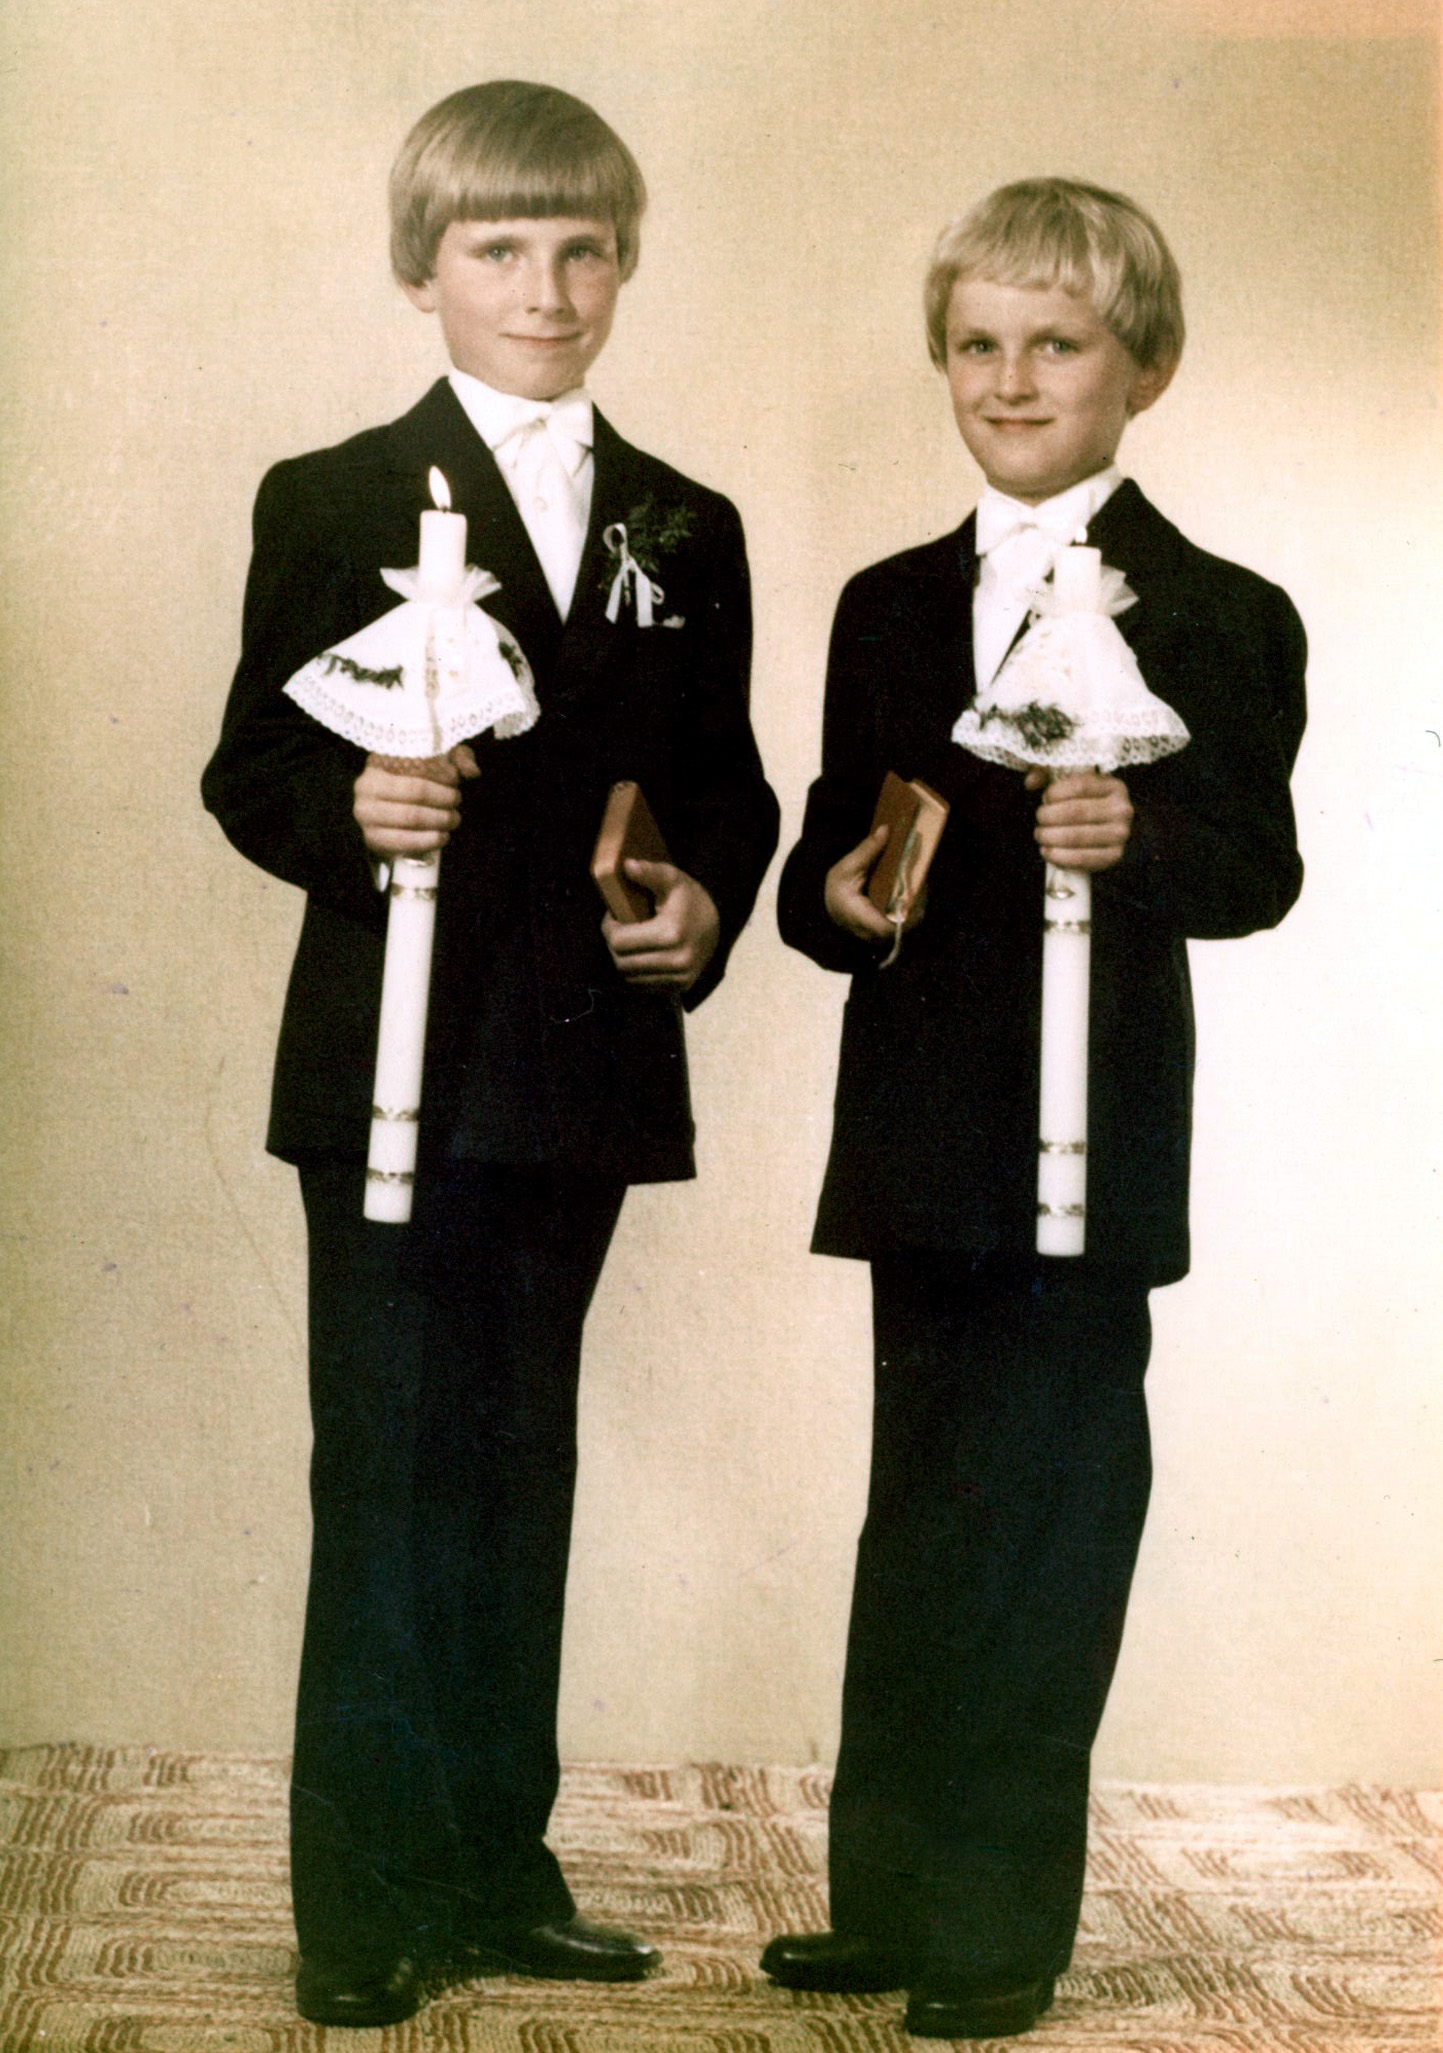
\includegraphics[width=0.35\textwidth]{photo/krzysztof_tomasz_lehman.jpg}
\caption{Krzysztof i Tomasz Lehmanowie u I Komunii św. }
\label{rys:krzysztof_tomasz_lehman}
\end{center}
\end{figure}

Grzegorz ukończył Zarządzanie i Marketing, ale pracuje w Kopalni Węgla Kamiennego ,,Pniówek'' w Pawłowicach. Nie ożenił się i mieszka przy matce w Ćwiklicach.

\begin{figure}[!h]
\begin{center}
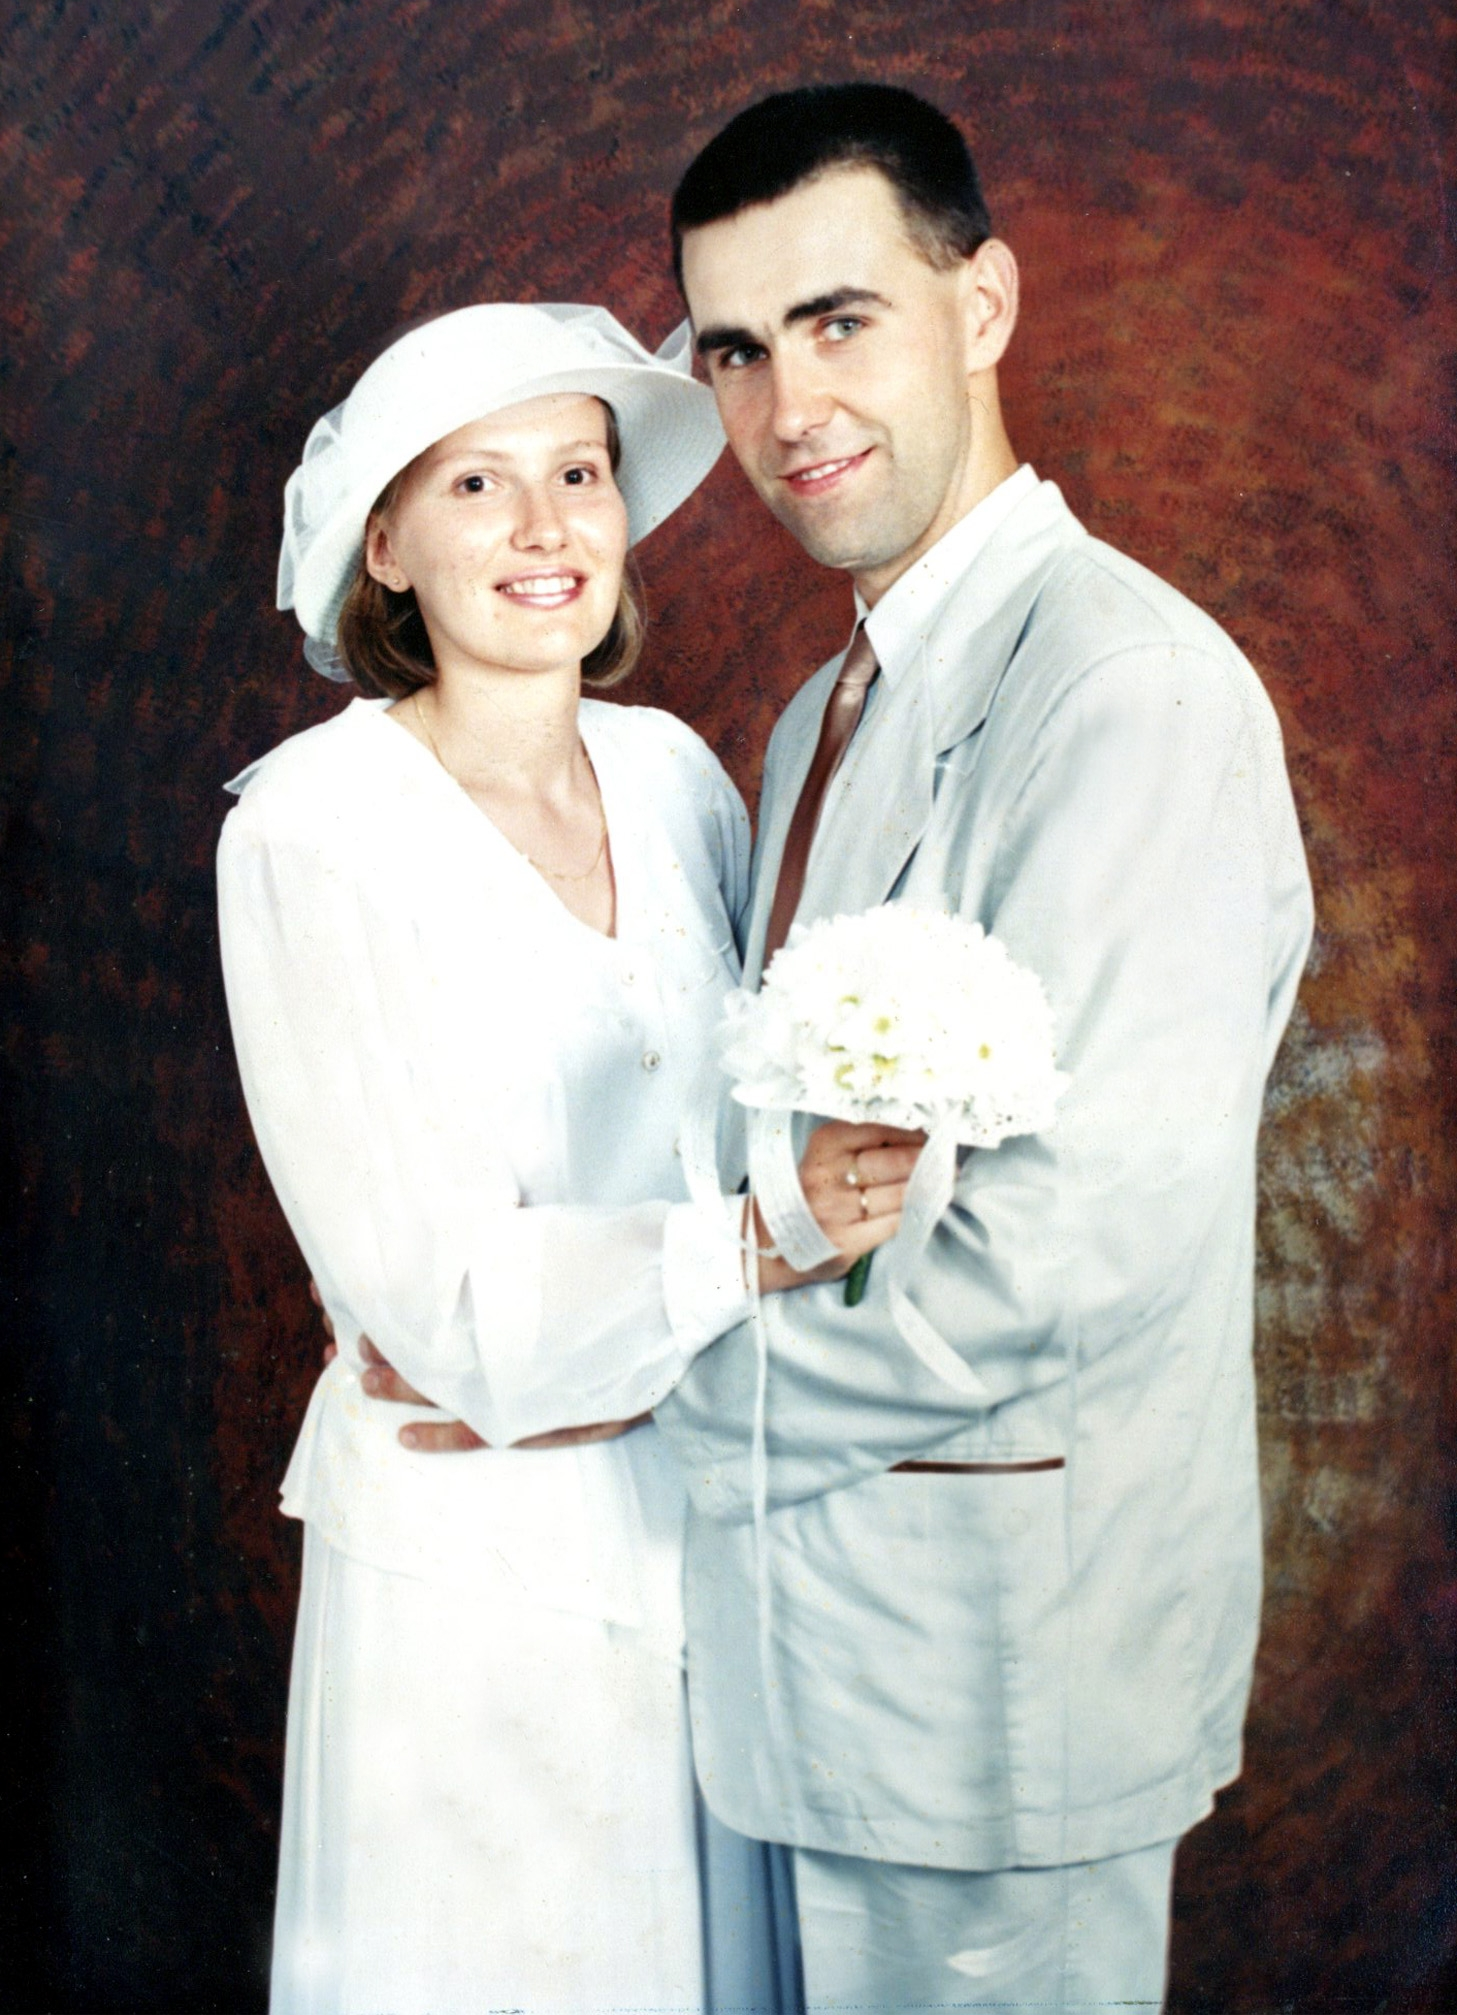
\includegraphics[width=0.4\textwidth]{photo/agnieszka_andrzej_lehman_slub.jpg}
\caption{Ślub Agnieszki Zdrojewskiej i Andrzeja Lehmana}
\label{rys:agnieszka_andrzej_lehman_slub}
\end{center}
\end{figure}

Andrzej ukończył Technikum Elektryczne i będąc na czwartym roku studiów wyjechał na Kretę, gdzie pracował na czarno. Tam poznał \textbf{Agnieszkę Zdrojewską urodzoną 13 listopada 1966 r. we Włocławku, córkę Zdzisława i Ireny Zdrojewskich. Pobrali się 8 czerwca 1991 r. w Chanii na Krecie.}

\begin{figure}[!h]
\begin{center}
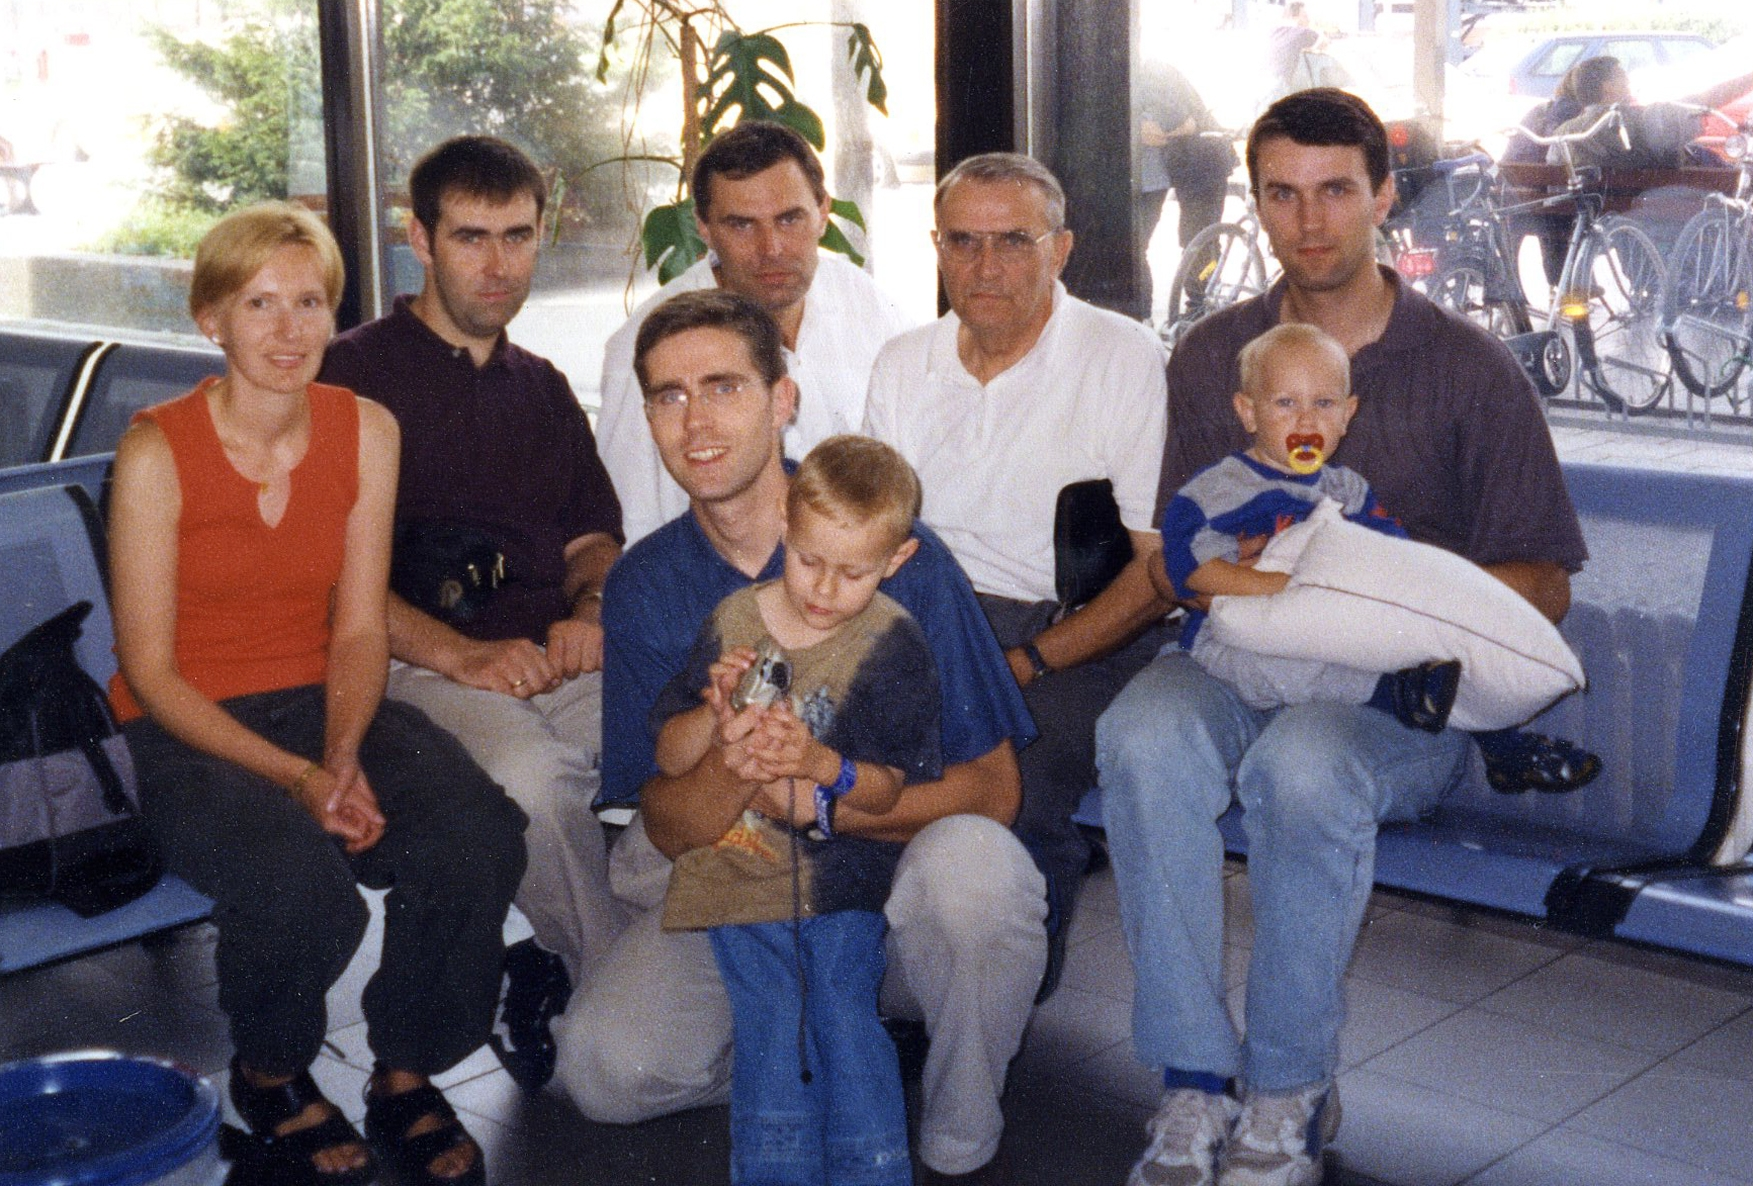
\includegraphics[width=0.6\textwidth]{photo/tadeusz_lehman_z_wnukami.jpg}
\caption[Tadeusz Lehman z wnukami]{Tadeusz Lehman z wnukami. Na zdj. od lewej siedzą: Agnieszka z Andrzejem, Grzegorz, ich ojciec i teść Tadeusz, Tomasz z małym Tomkiem, a przed nimi kuca Krzysiu z małym Konradem.}
\label{rys:tadeusz_lehman_z_wnukami}
\end{center}
\end{figure}

Potem był epizod próby wykiwania władz Republiki Federalnej Niemiec i wreszcie bezpieczne wraz z żoną osiedlenie w \textbf{Edmonton} -- półmilionowym mieście uniwersyteckim w zachodniej Kanadzie, gdzie pracuje jako elektryk. Tam przyszli na świat ich dwaj synowie, a prawnukowie stryjenki Ireny: \textbf{Konrad -- 11 sierpnia 1995 r. oraz Tomasz -- 17 lutego 1999 r}. Przed śmiercią Tadeusz zdążył jeszcze odwiedzić swego syna, synową i wnuków w Edmonton.

\begin{figure}[!h]
\begin{center}
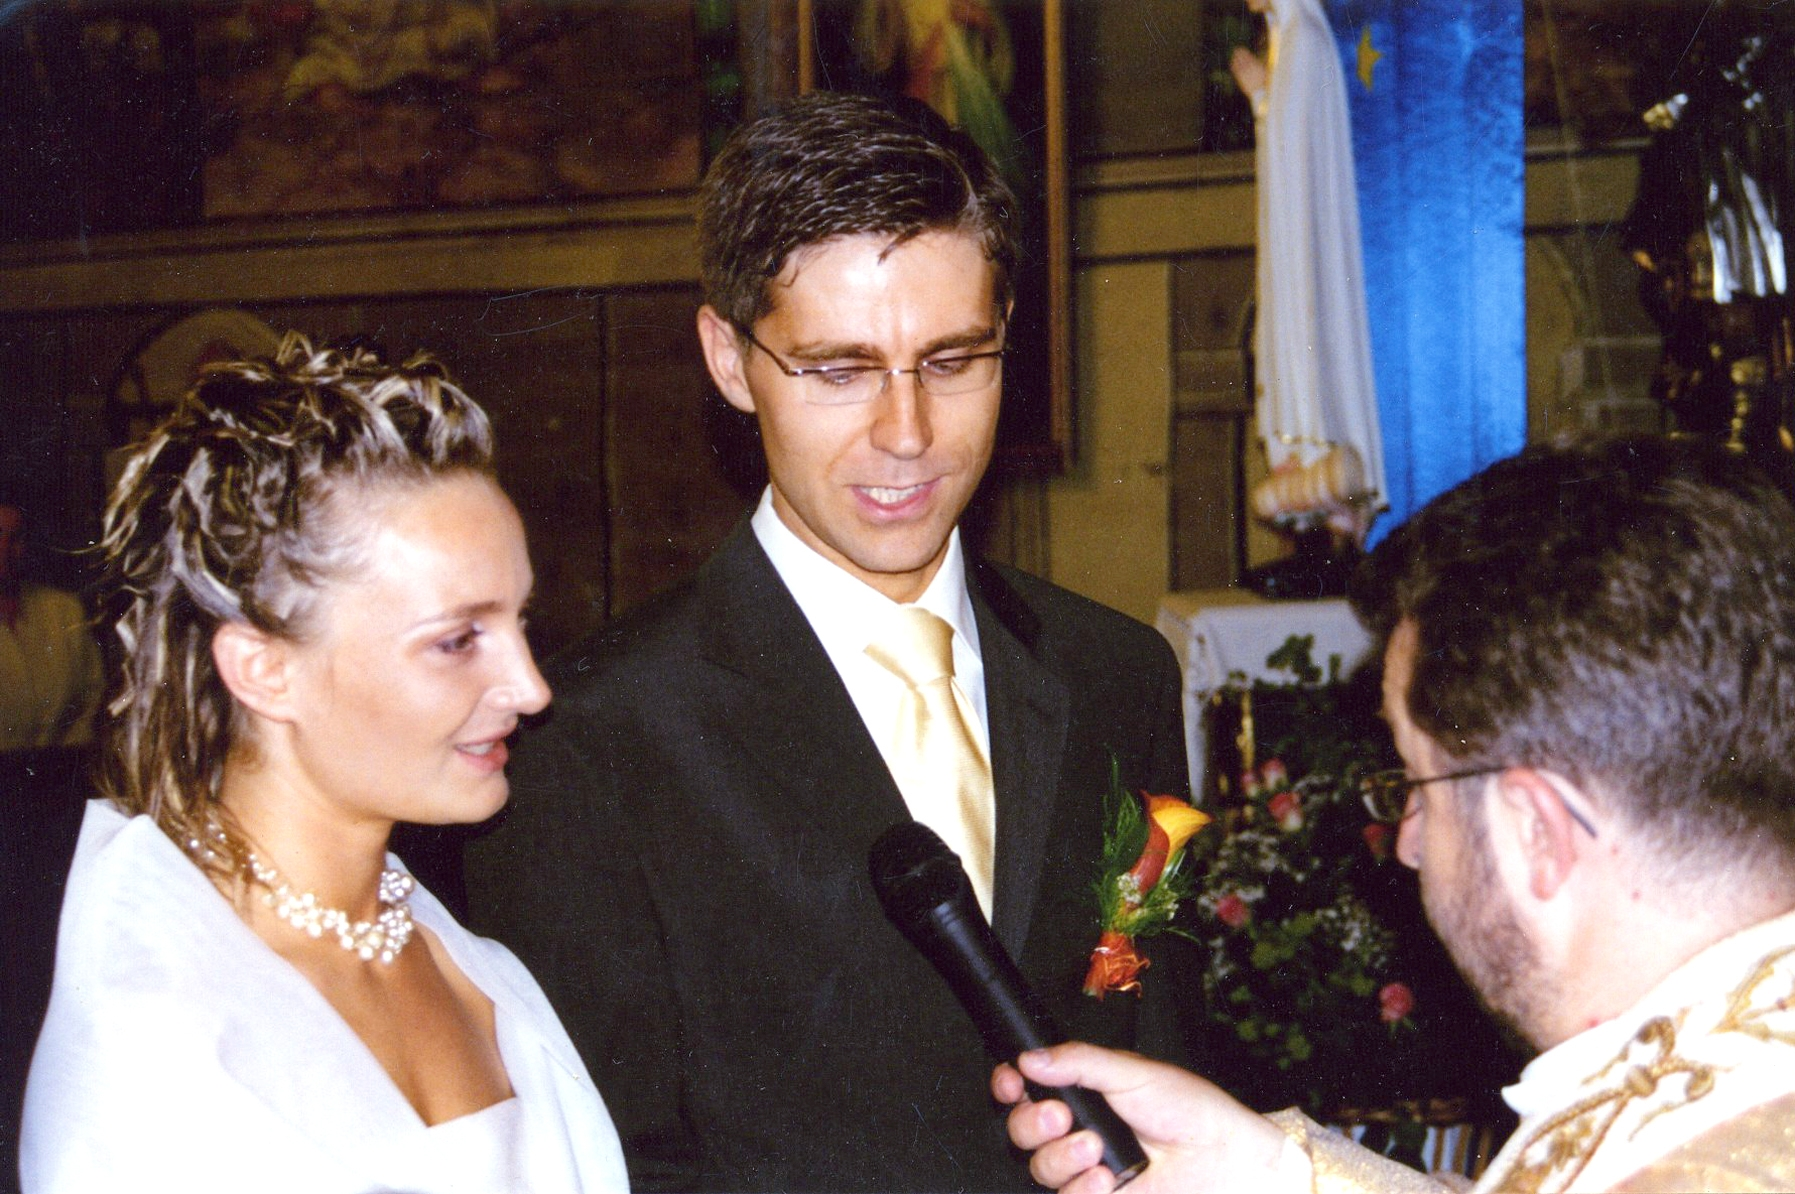
\includegraphics[width=0.6\textwidth]{photo/krzysztof_zofia_lehman_slub.jpg}
\caption{Ślub Zofii Wyrobek i Krzysztofa Lehmana}
\label{rys:krzysztof_zofia_lehman_slub}
\end{center}
\end{figure}

Krzysztof Lehman ukończył informatykę na Politechnice Gliwickiej w Katowicach i pracuje w NETIA S.A. w Warszawie. \textbf{Ożenił się w Ćwiklicach 24 lipca 2004 r. z Zofią Wyrobek -- córką Andrzeja i Janiny z domu Urbańczyk urodzoną 24 września 1979 r. w Pszczynie.}

Ukończyła ona filologię romańską na Uniwersytecie Śląskim i pracuje w Leroy Merlin w Warszawie. Mieszkają w Warszawie przy ul. Hektarowej 2B/5.
\textbf{2 czerwca 2009~r. w Warszawie przyszedł na świat ich syn Piotr.}

\textbf{Tomasz Lehman}, podobnie jak Grzesiu, ukończył Zarządzanie i Marketing i pracuje w Telekomunikacji Kopalń Piasku. Mieszka, jak Grzegorz przy mamusi w Ćwiklicach. 

\begin{figure}[!h]
\begin{center}
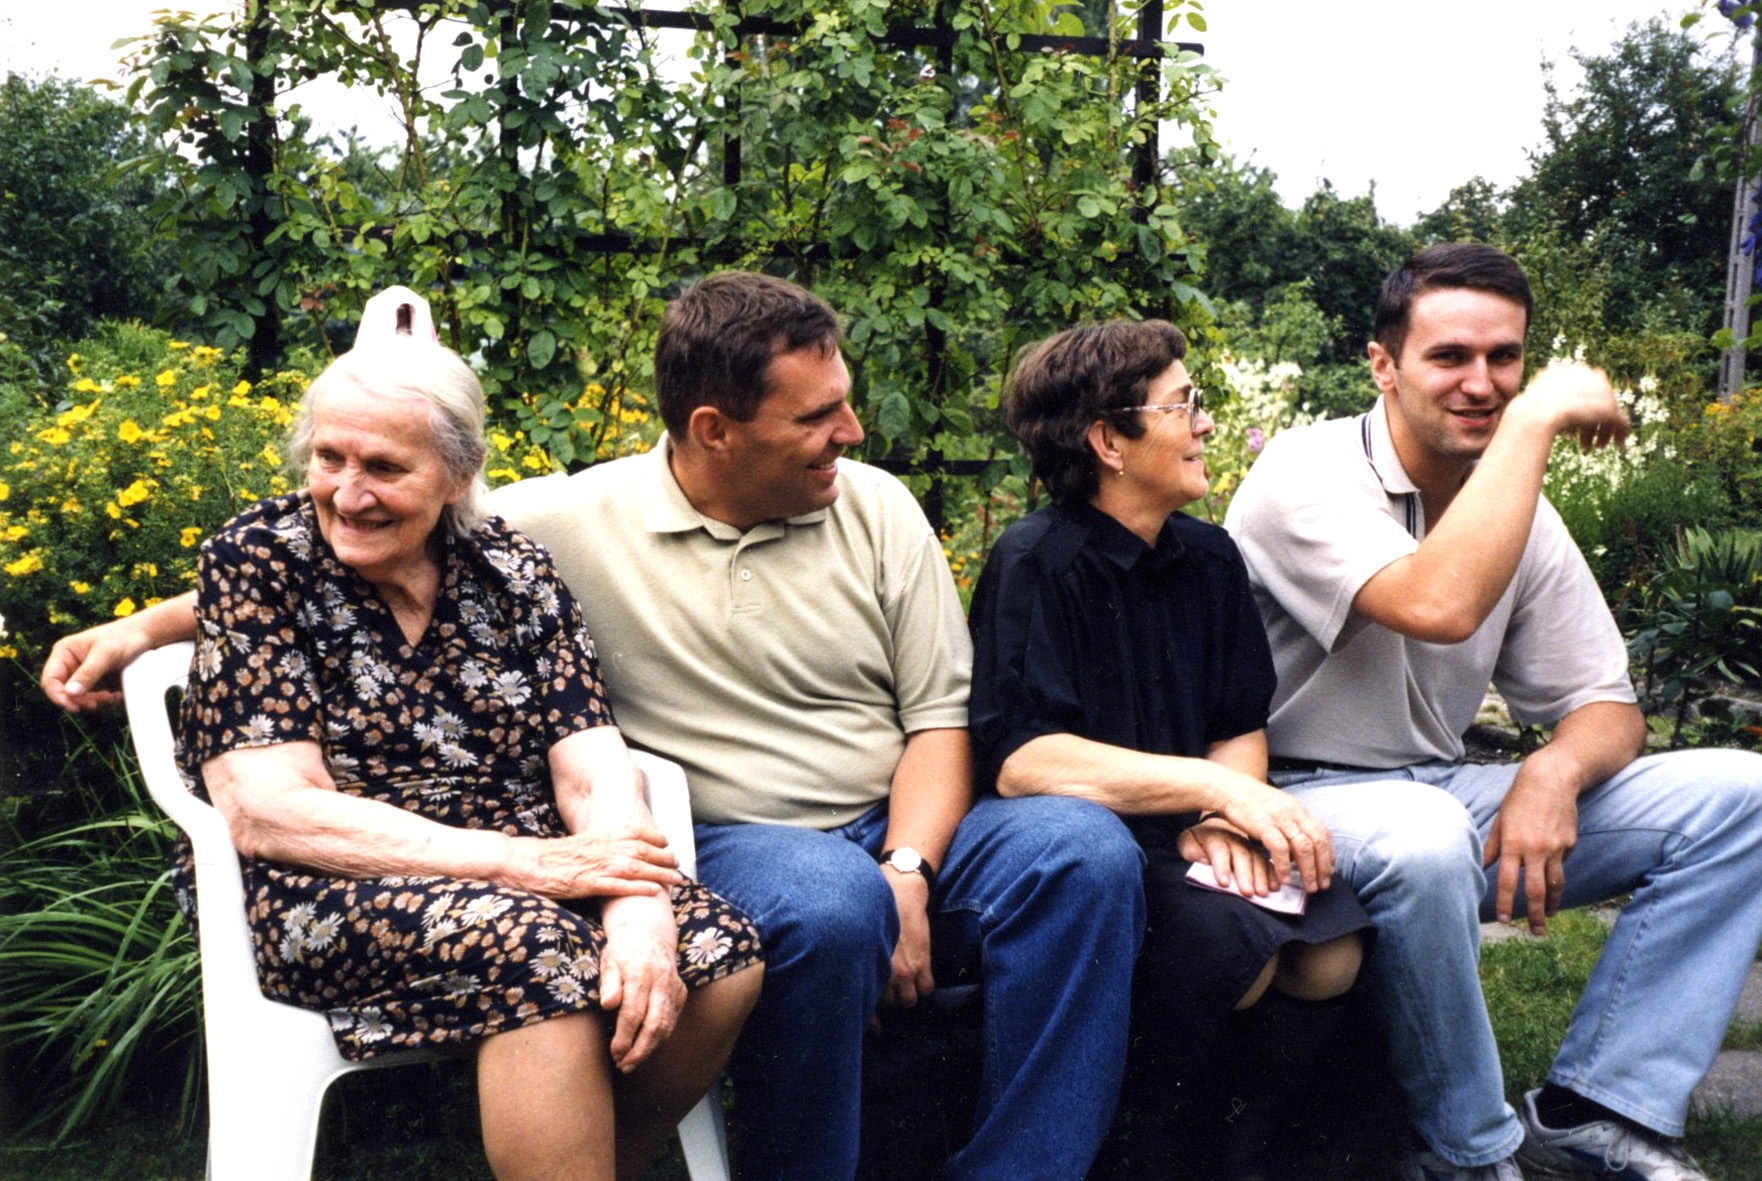
\includegraphics[width=0.6\textwidth]{photo/grzegorz_tomasz_lehman.jpg}
\caption[Irena Lehman z wnukiem Grzegorzem, synową Lubomirą i wnukiem Tomaszem Lehmanem]{Na zdj. Irena Lehman z wnukiem Grzegorzem, synową Lubomirą i wnukiem Tomaszem Lehmanem.}
\label{rys:grzegorz_tomasz_lehman}
\end{center}
\end{figure}

Tadeusz z Lubomirą najpierw mieszkali przy jej rodzicach w Ćwiklicach, a następnie w Tychach. W tym czasie budowali dom w Ćwiklicach, w co bardzo mocno zaangażował się stryj Antoni i finansowo i ogromnym wkładem pracy w nadziei, że będzie mógł tam przy wdzięcznych dzieciach dokonać żywota. Jak gorzko się omylił, kiedy po latach ciężkiej pracy na budowie syna, po tylu wyrzeczeniach, by ze swoich skromnych zarobków wspomóc tę budowę finansowo, dowiedział się od swojej synowej, że nie przewiduje się miejsca dla niego i jego małżonki w tym przez niego zbudowanym domu. Stryj Antoni zawsze chętnie niosący pomoc, o czym mogłem się wielokrotnie przekonać w Łagiewnikach na Wieskach, gdzie miał ręce pełne roboty mimo podeszłego wieku -- dotknięty w swym honorze do żywego do końca życia nie pojawił się już więcej w Ćwiklicach!\ldots

\begin{figure}[!h]
\begin{center}
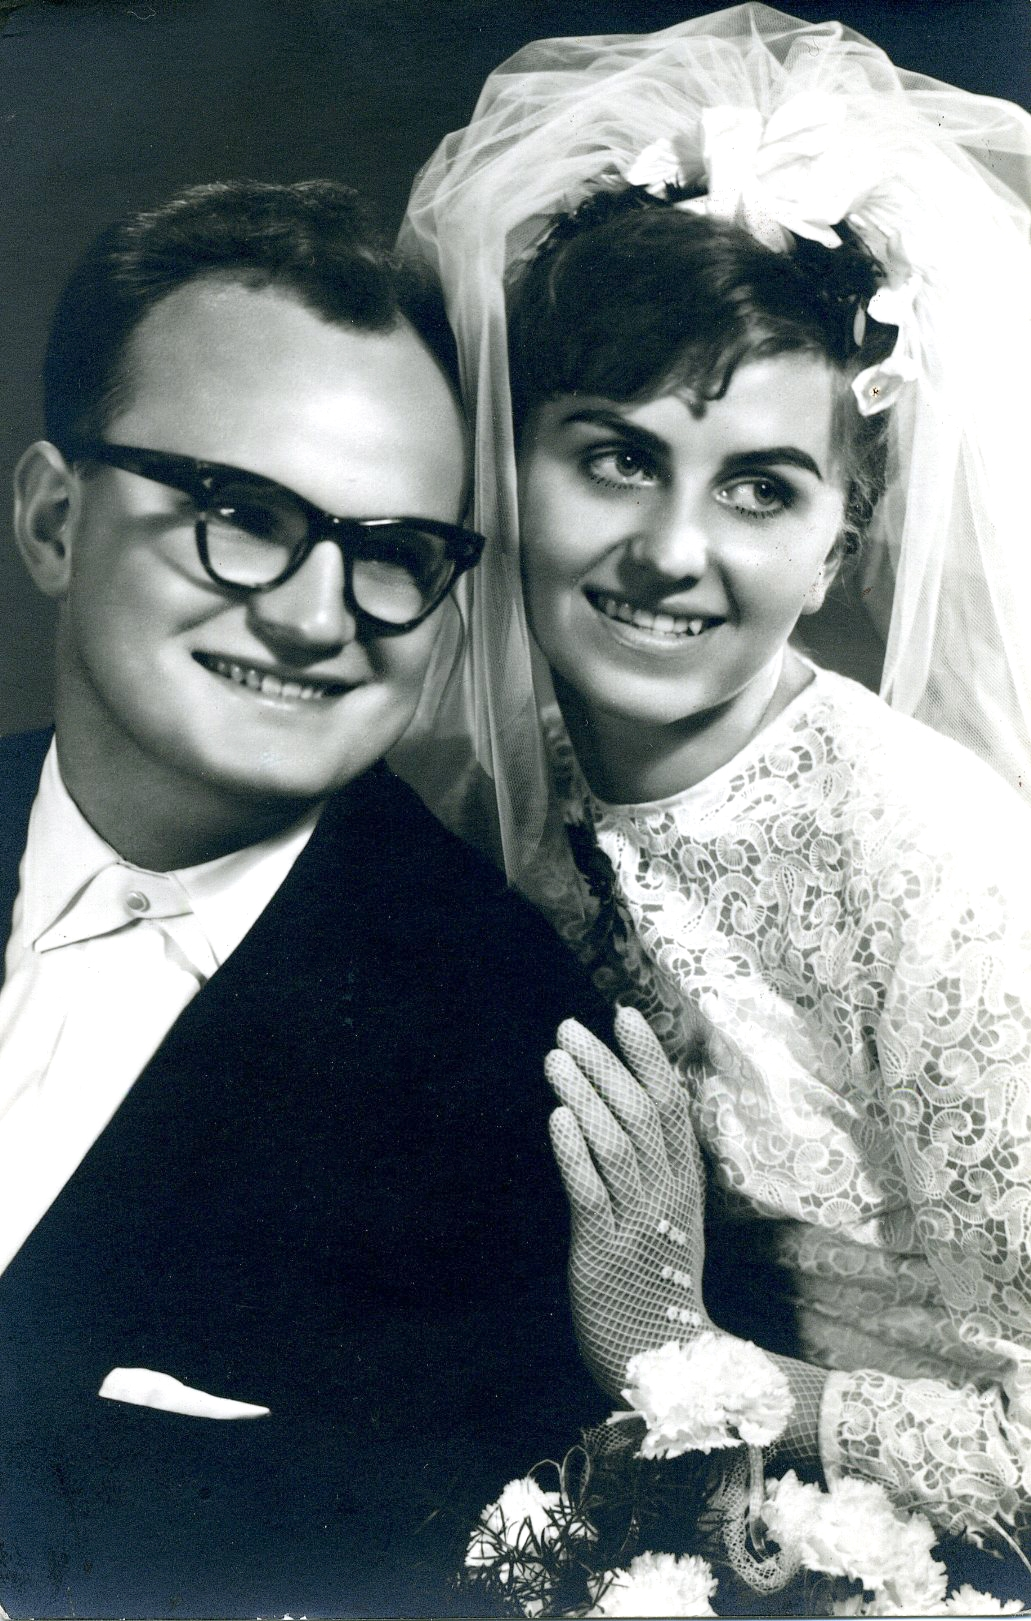
\includegraphics[width=0.35\textwidth]{photo/gustaw_marta_lehman_slub.jpg}
\caption{Ślub Marty Skudło i Gustawa Lehmana}
\label{rys:gustaw_marta_lehman_slub}
\end{center}
\end{figure}

O pięć lat młodszy od Tadeusza \textbf{Gustaw} ukończył w Tychach Technikum Mechaniczne w klasie obróbki skrawaniem i zatrudnił się w Zakładzie Elektroniki Górniczej w ,,Narzędziowcu'', a następnie w Przedsiębiorstwie Energetyki Cieplnej Sieciowej w Tychach oraz w MZUiM w Tychach i wreszcie we ,,Fiacie'', najpierw w Bielsku Białej, a następnie w Tychach. Był tam głównym mechanikiem oraz szefem utrzymania ruchu. \textbf{Ożenił się w Tychach w kościele farnym p.w. św. Marii Magdaleny dnia 20 czerwca 1964 r. z Martą Skudło urodzoną 5 marca 1941 r. w Tychach -- Paprocanach, córką Stefana i Weroniki z domu Jędrysik.} Ukończyła ona Liceum Ogólnokształcące i podjęła pracę w Piezoelektronice, późniejszym ZEG-u. Mieszkali w mieszkaniu spółdzielczym -- najpierw w bloku przy ul. Wieczorka (na 3 piętrze), a następnie w bloku przy ul. Brzozowej 14a w Tychach. \textbf{Gustaw zmarł nagle 7 czerwca 1999~r.} na tętniaka w brzuchu, który pękł.

Krwi upłynęło mnóstwo, ale dowieźli go do szpitala żywego. Operacja się udała, jednak wkrótce urwał się skrzep, który spowodował śmiertelny zator serca. Nie mogła tego przeboleć \textbf{Marta -- jego żona, która tak bardzo się stęskniła, że 25 grudnia 2005 r. poszła za nim ścięta rakiem}\ldots Nie poddała się jednak bez walki, działała w Stowarzyszeniu Amazonek, lecz gdy nastąpiły przerzuty odeszła w pełni świadoma.

\textbf{Doczekali się 8 października 1965 r. wspaniałego syna Marka urodzonego u Babki w Katowicach Bogucicach}, który wziął po ojcu posturę i czuprynę. Ukończył on w 1990 r. studia na Akademii Rolniczej w Krakowie na Wydziale Melioracji Wodnych. Poznał tam śliczną myszkowiankę -- \textbf{Małgorzatę Górkę -- córkę Tadeusza i Alicji z domu Kapuściak urodzoną w Myszkowie 24 lipca 1964 r.}

\begin{figure}[!h]
\begin{center}
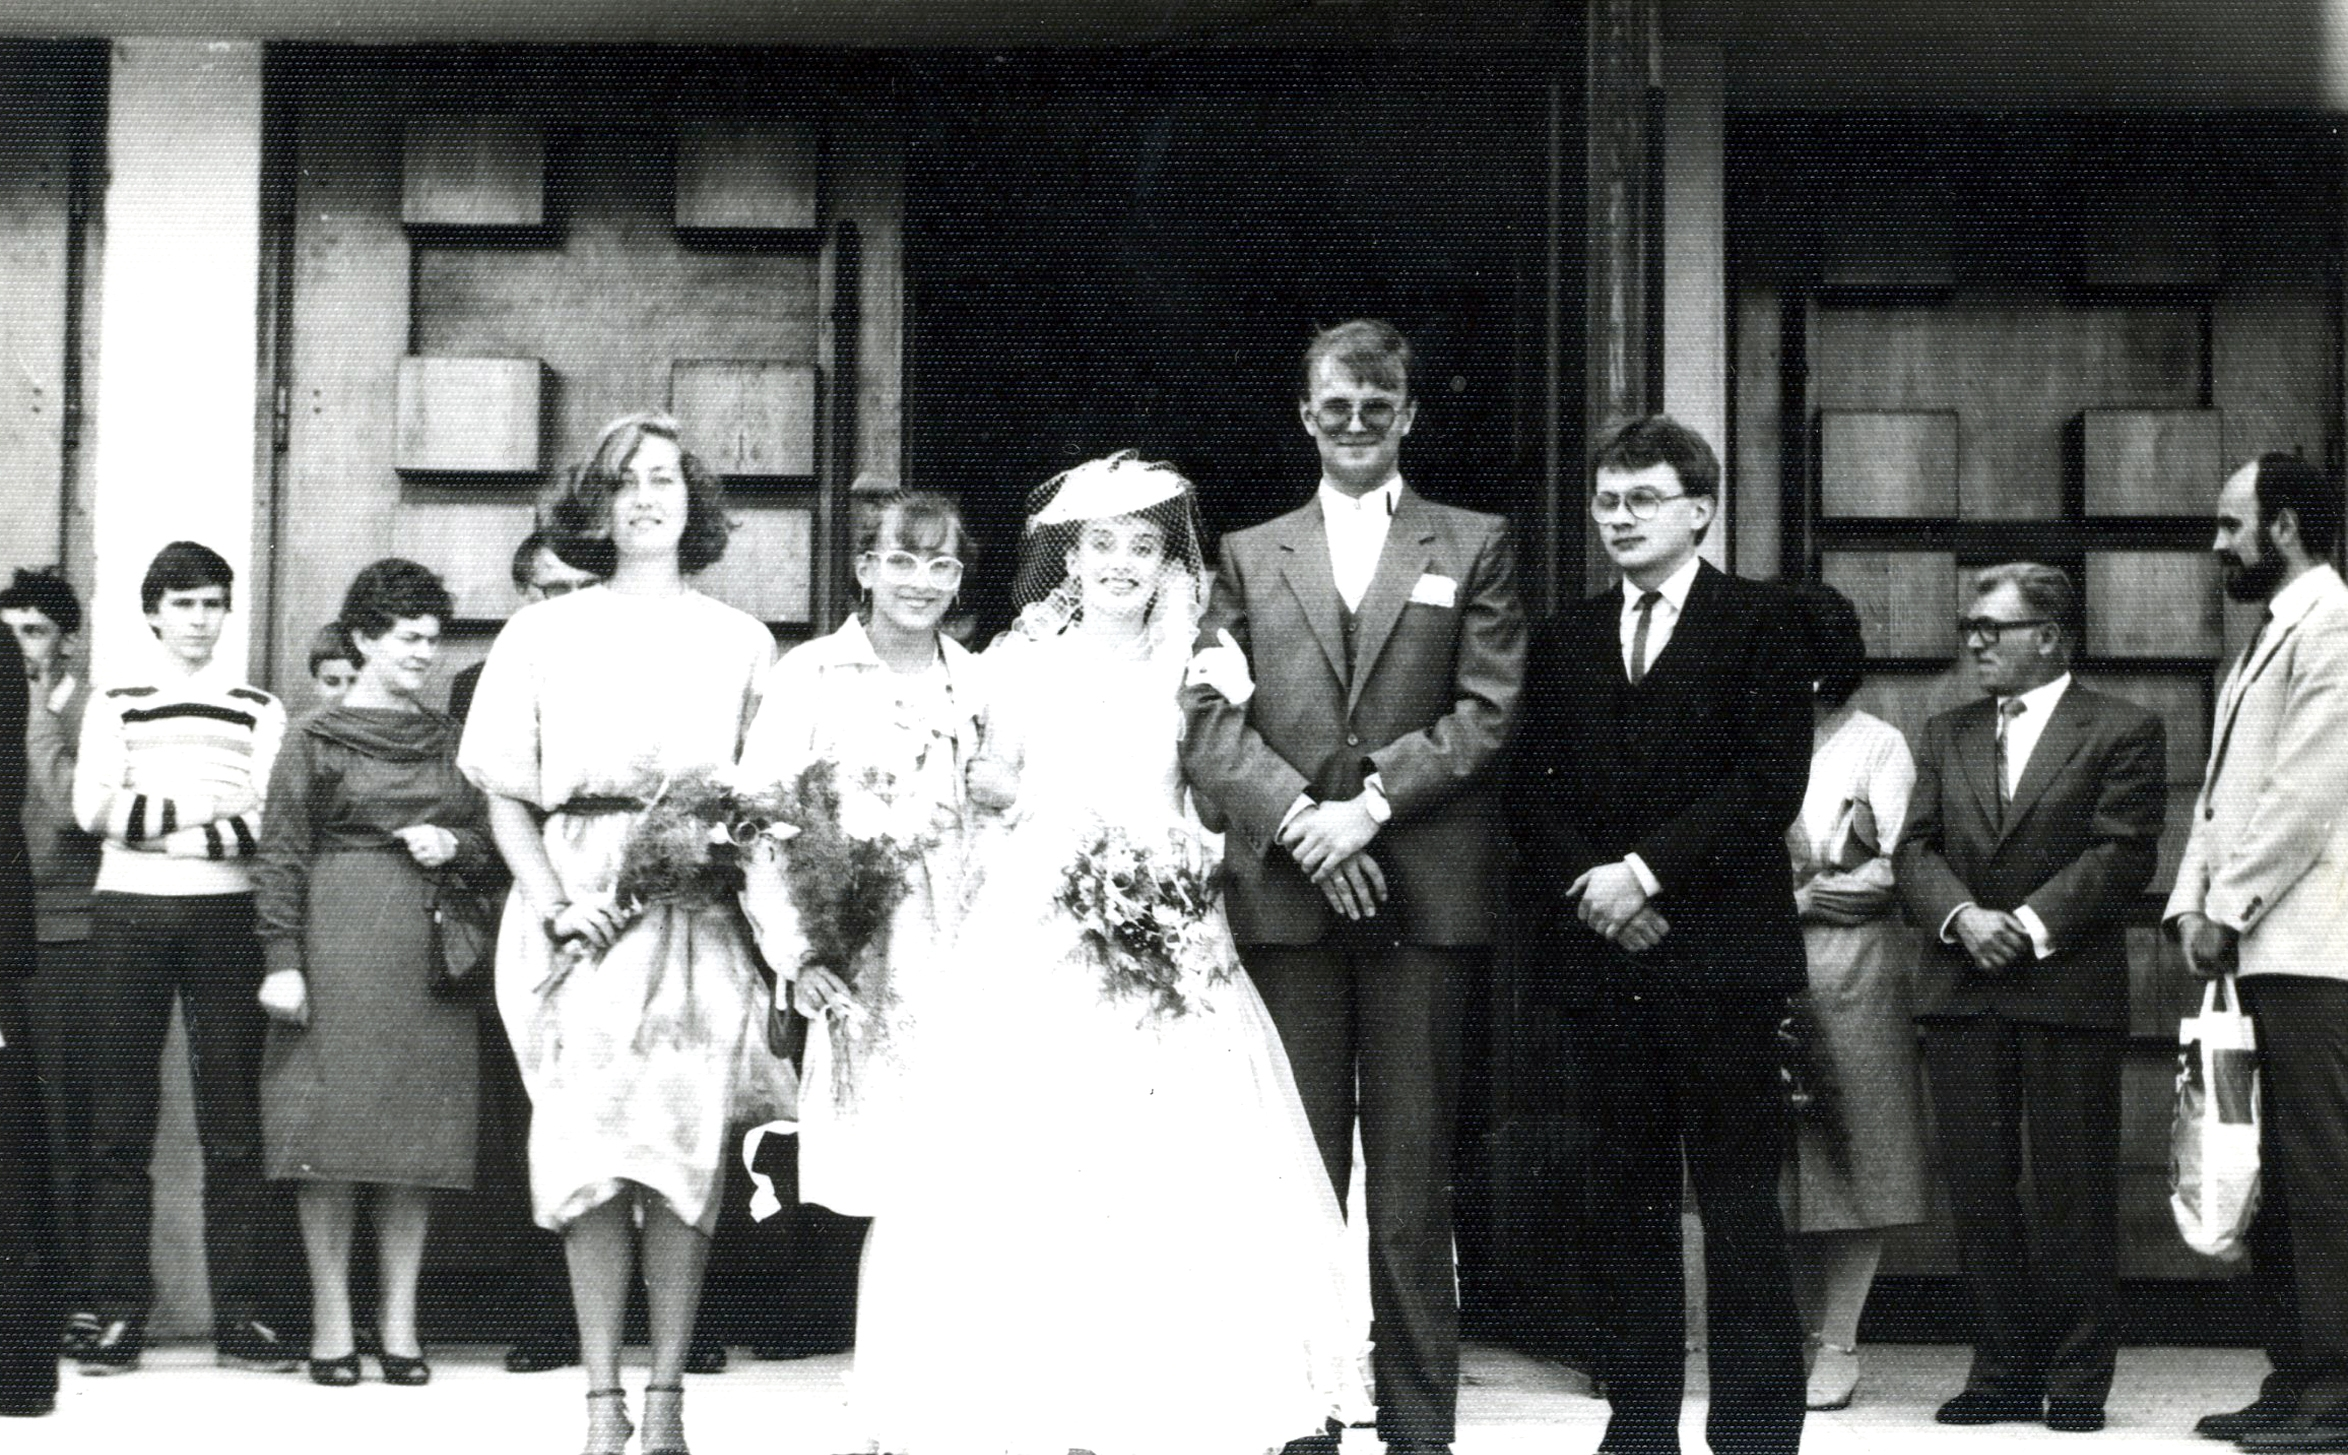
\includegraphics[width=0.7\textwidth]{photo/marek_malgorzata_lehman_slub.jpg}
\caption{Ślub Małgorzaty Górki i Marka Lehmana}
\label{rys:marek_malgorzata_lehman_slub}
\end{center}
\end{figure}

\textbf{Pobrali się w czasie studiów w USC w Myszkowie 9 lipca 1986 r., a ślub kościelny wzięli w Tychach Czułowie 20 sierpnia 1986 r.}

Młodzi zamieszkali najpierw w Tychach przy ul. Brzozowej u rodziców Marka, a następnie wynajmowali dwa pokoje w familoku przy ul Bałuckiego. Doczekali się dwóch synów: \textbf{Doriana ur. 6 stycznia 1987 r. w Katowicach i Jakuba ur. 18 marca 1993 r. również w Katowicach u babki Lehmanki}.

\begin{figure}[!h]
\begin{center}
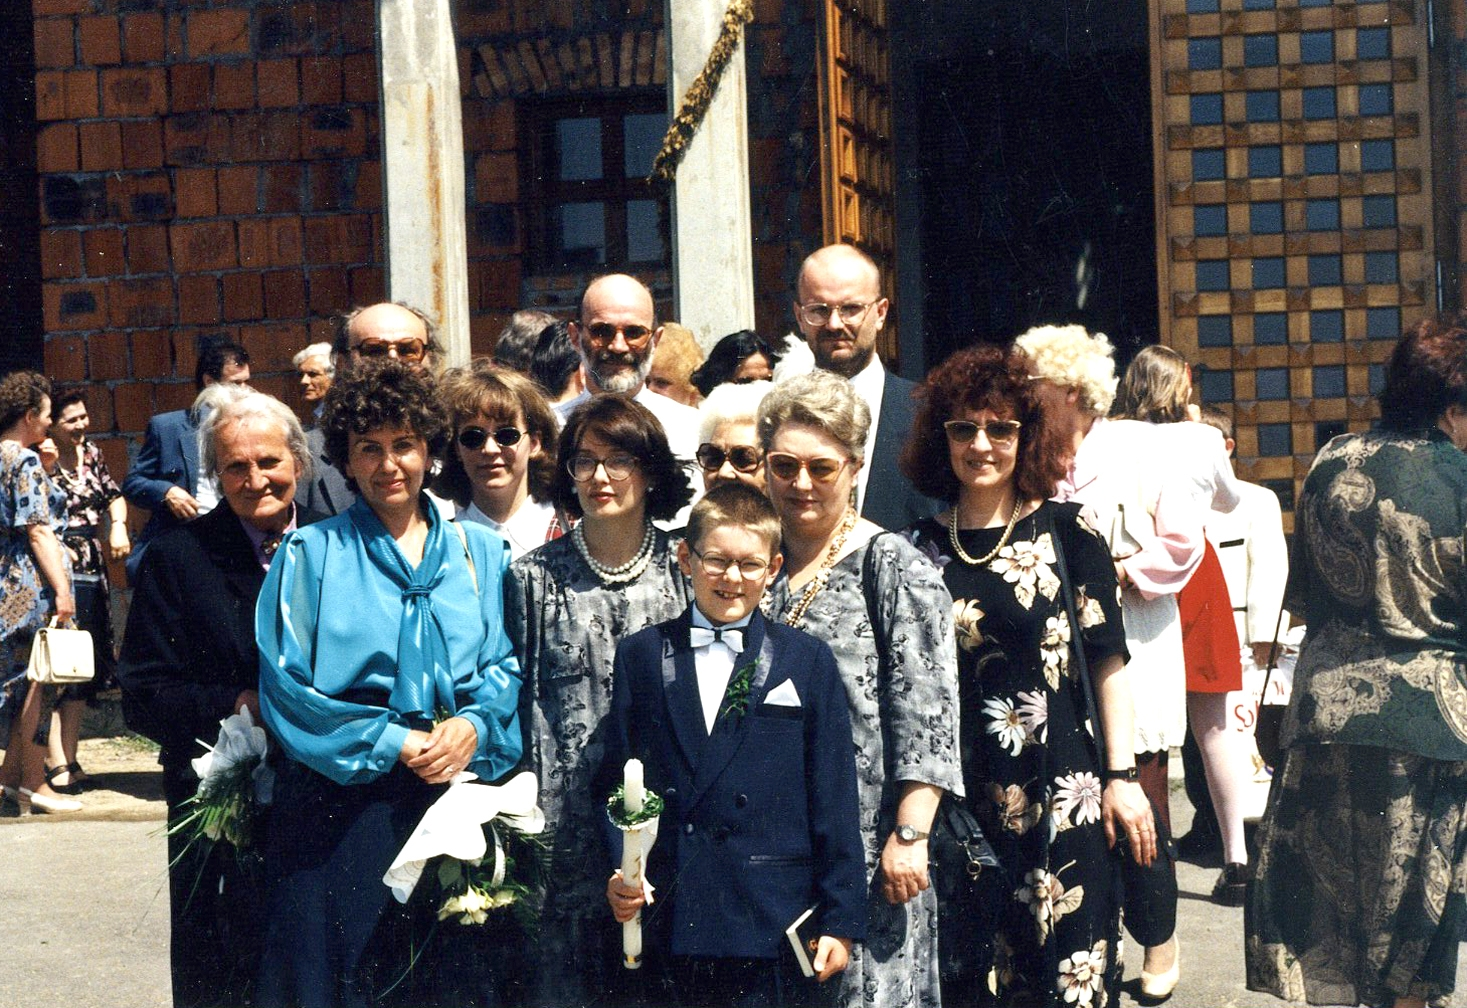
\includegraphics[width=0.7\textwidth]{photo/dorian_lehman_komunia.jpg}
\caption[Pierwsza Komunia św. Doriana Lehmana]{Pierwsza Komunia św. Doriana Lehmana. Na zdj. od lewej: Prababka Irena Lehman, Marta Lehman (babka Doriana), za nią Gustaw Lehman (dziadek Doriana), obok Boguś Lehman i Marek Lehman (ojciec Doriana), tuż za Dorianem jego mama Małgorzata.}
\label{rys:dorian_lehman_komunia}
\end{center}
\end{figure}

Wkrótce przeprowadzili się do trzypokojowego mieszkania przy ul. Begonii, które wynajmowali. Nagle właścicielka tego lokalu zmieniła drastycznie warunki najmu, żądając alternatywnie jego wykupu za tak wielkie pieniądze, że mogli za nie kupić dom z działką, co też uczynili i zamieszkali w Łące pod Pszczyną. Nabyty przez nich dom nie był jeszcze wykończony, więc pierwsze miesiące mieszkali w iście spartańskich warunkach. Wytrzymali, dom wykończyli i doposażyli.

\begin{figure}[!h]
\begin{center}
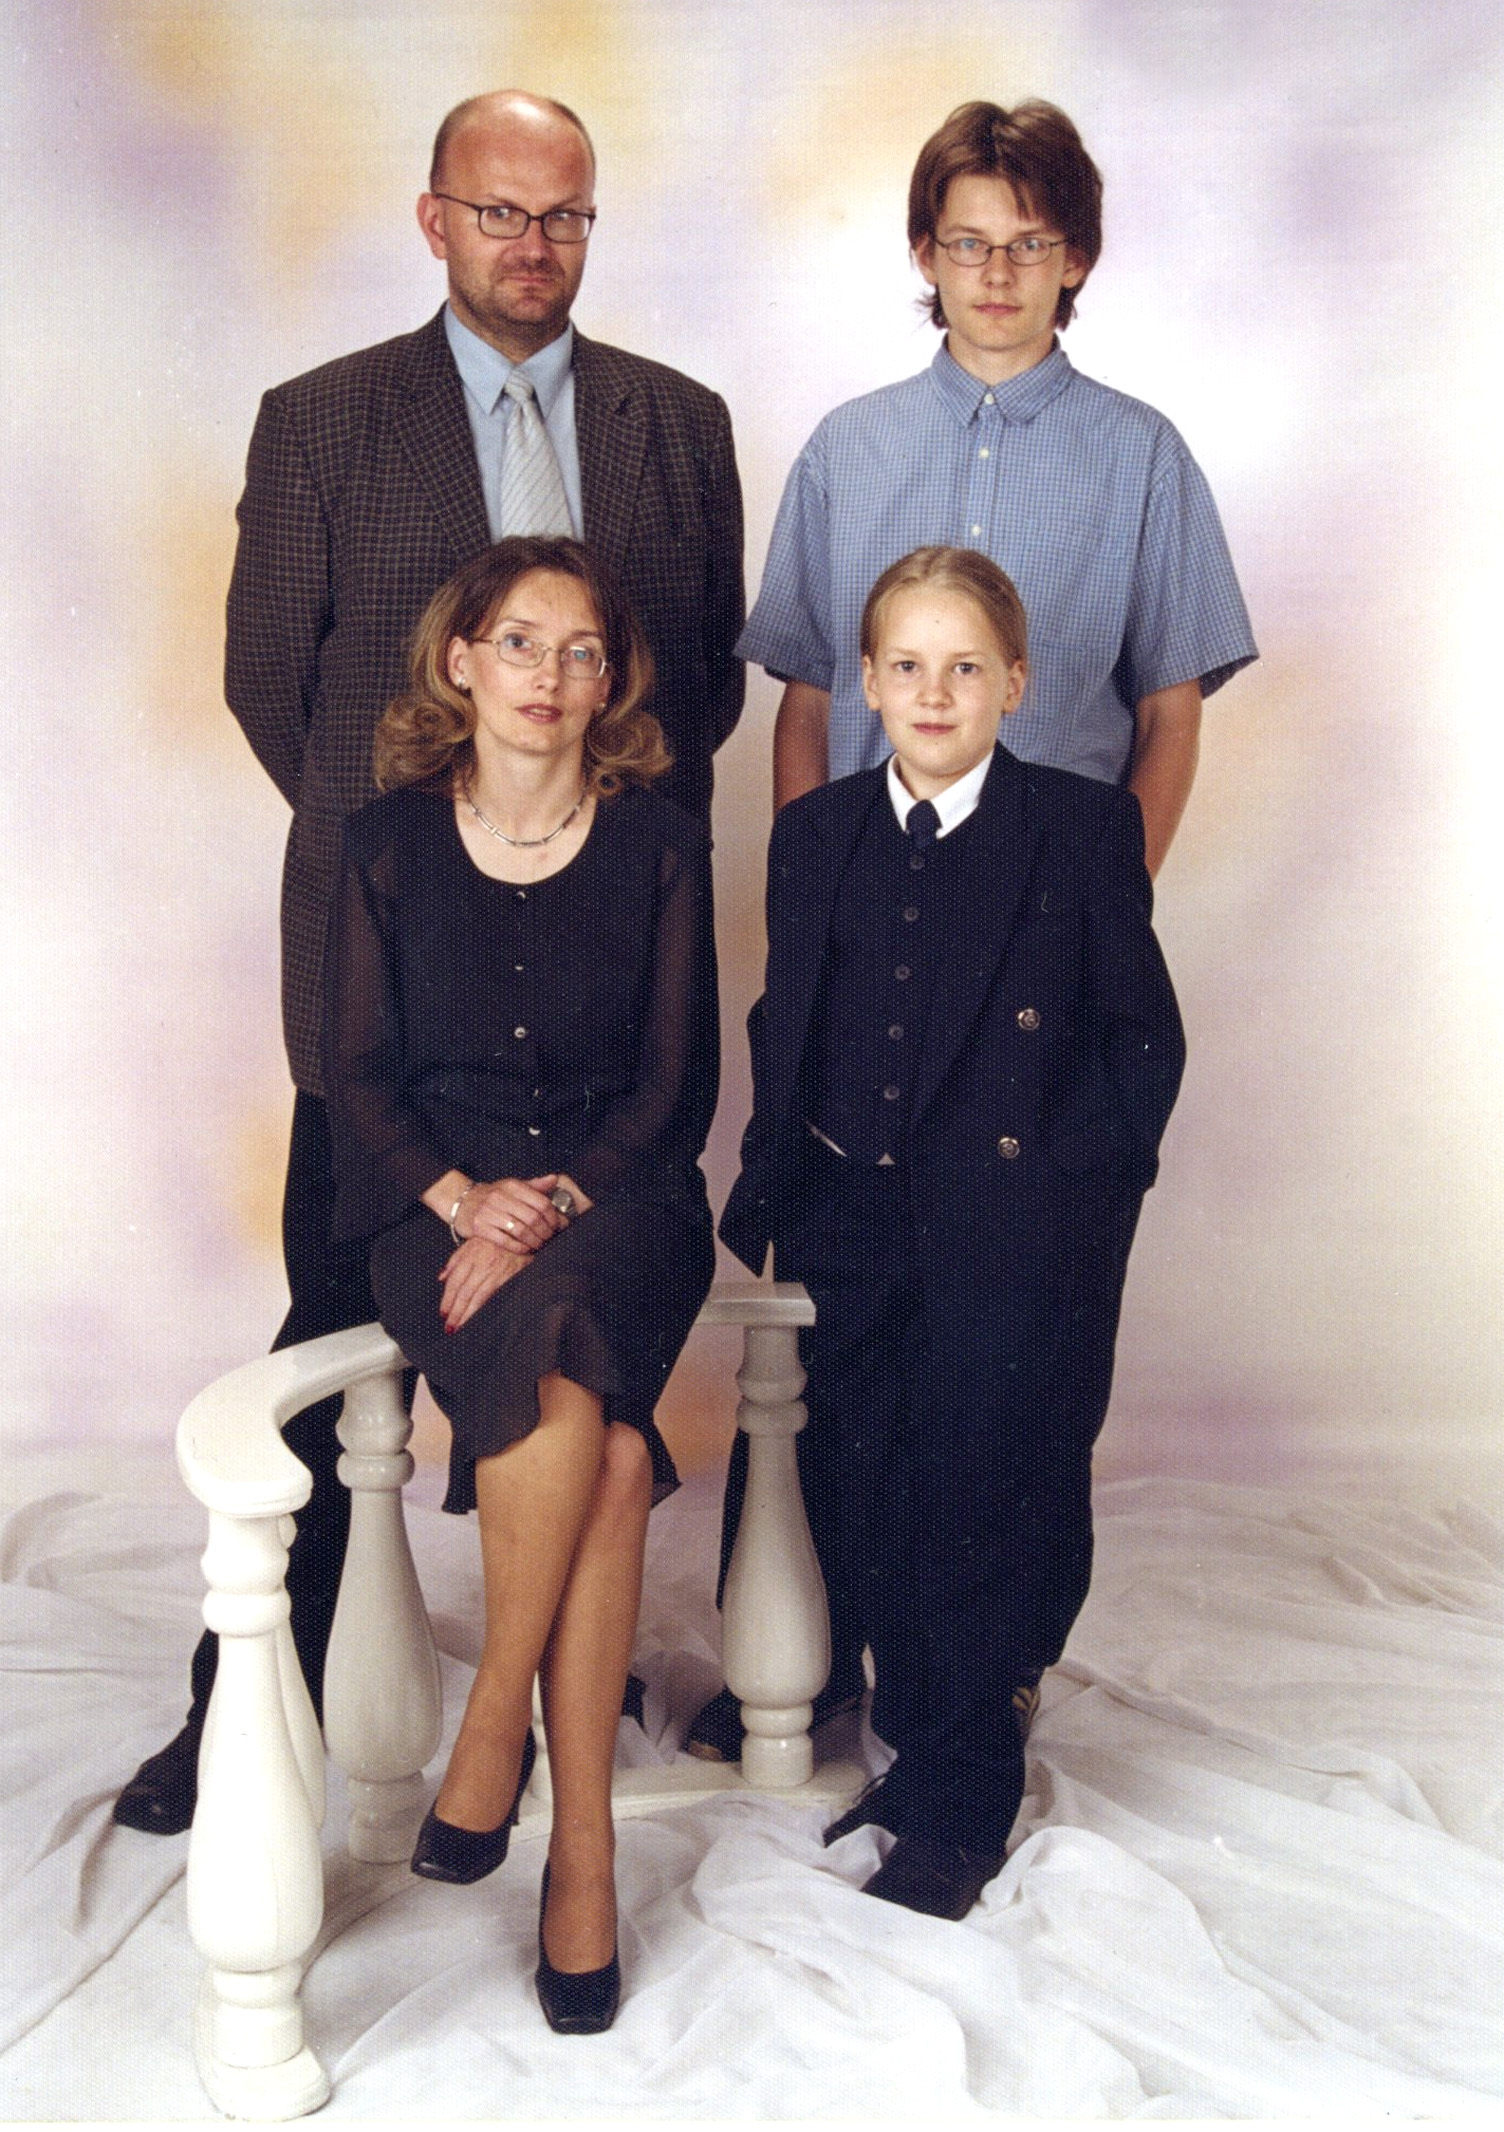
\includegraphics[width=0.4\textwidth]{photo/marek_malgorzata_lehman_z_dziecmi.jpg}
\caption{Marek i Małgorzata Lehman z synami: Dorianem i Jakubem.}
\end{center}
\end{figure}

Jednak, gdy nadarzyła się okazja  nabycia pięknego domu w samej Pszczynie przy ul. Studzienickiej 44, skorzystali z niej i tam teraz szczęśliwie mieszkają.

Zaraz po studiach Marek podjął pracę w Górnośląskim Banku Gospodarki Rolnej w Katowicach, a następnie w Śląskim Domu Maklerskim (licencję maklera papierów wartościowych uzyskał w 1993 r.). Po wygranym konkursie Marek zatrudnił się w Grupie Inwestycyjnej ROHA, gdzie pracował 4 lata uzyskując spore dochody, lecz w domu będąc gościem (2 dni pracował w Katowicach, dwa dni w Warszawie, dzień w Lublinie i dzień w Krakowie). Wybrał rodzinę i dlatego zatrudnił się w Węgloskładzie SA przy KWK ,,Czeczot'', gdzie pracował półtora roku. Potem zatrudnił się na 3 lata w Mostostalu w Będzinie, a następnie w Budostalu 6 w Dąbrowie Górniczej w latach 1999~-~2002. Od tego czasu, tj. od 2002~r. prowadzi własną działalność pod nazwą ,,Marek Lehman -- Biegły Sądowy'' w zakresie rachunkowości i finansów, z czego jest bardzo zadowolony.

Małgosia po wyjściu za mąż przerywa studia i podejmuje pracę w Zakładzie Elektroniki Górniczej w Tychach, gdzie pracuje do 1992 r. Potem, ukończywszy Szkołę Kosmetyczną, otworzyła Gabinet Kosmetyczny w Tychach na Żwakowie, o nazwie ,,Studio Kosmetyczne LM''. Gdy klientela nie dopisała podjęła pracę w Węgloskładzie, gdzie Marek piastował kierownicze stanowisko. Małgosia prowadząc dom,  jednocześnie studiowała na Akademii Sztuk Pięknych w Krakowie, którą ukończyła i obecnie wystawia swoje obrazy na wystawach w kraju i Europie.

\begin{figure}[!h]
\begin{center}
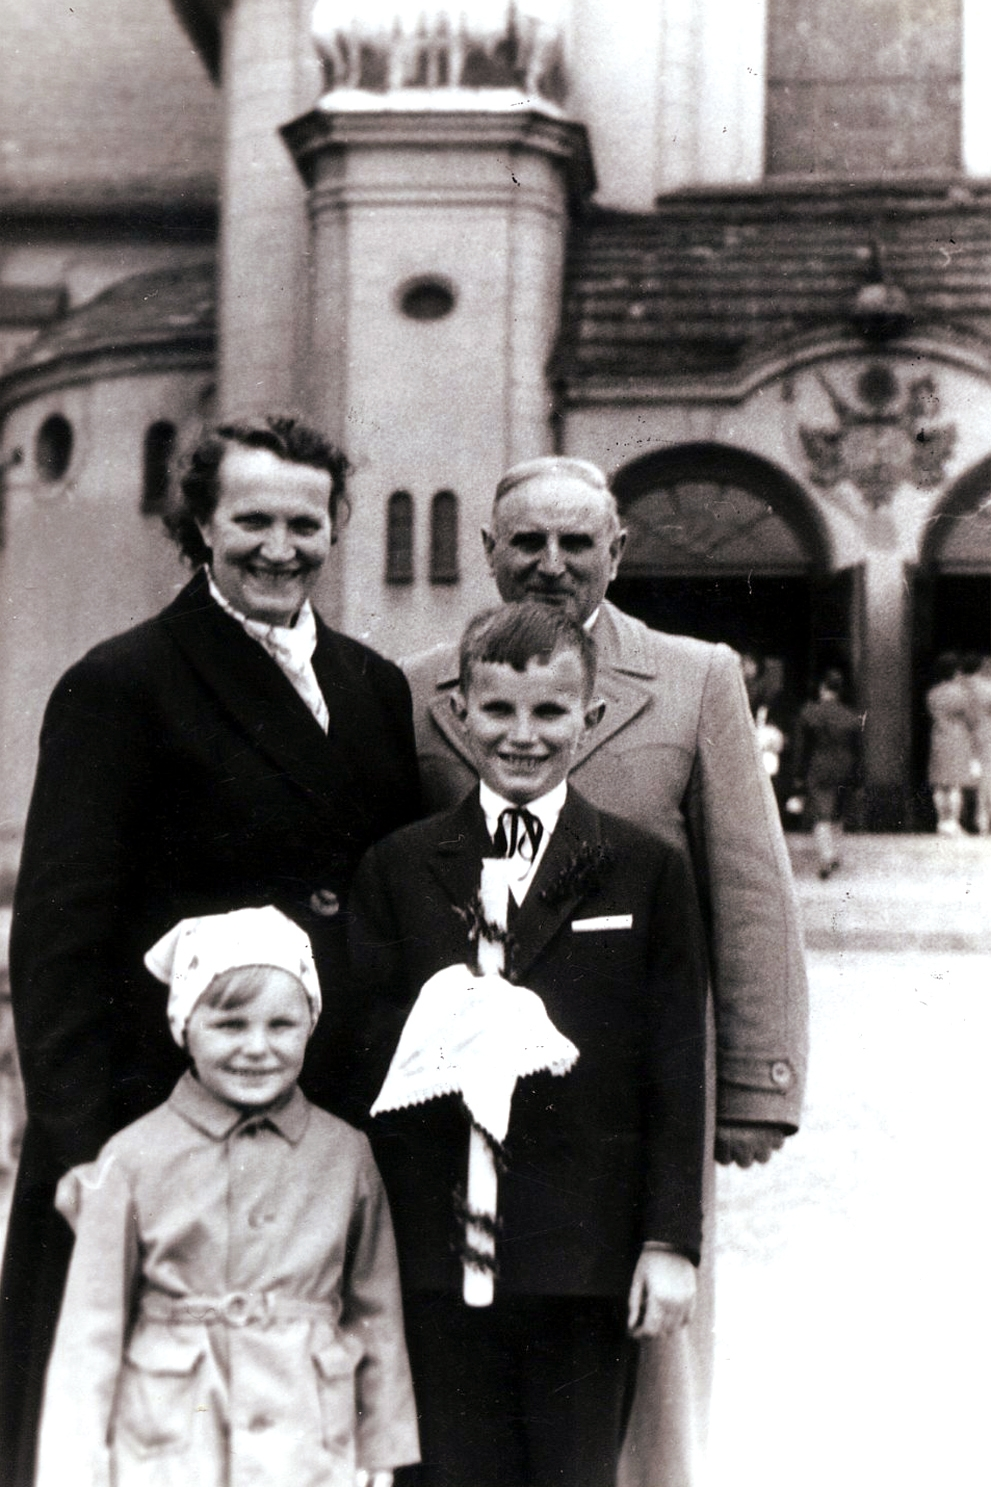
\includegraphics[width=0.4\textwidth]{photo/bogumil_lehman_komunia.jpg}
\caption[Pierwsza Komunia św. Bogumiła Lehmana]{Pierwsza Komunia św. Bogumiła Lehmana. Na zdj. z kuzynką Basią Kuś i rodzicami.}
\end{center}
\end{figure}

\textbf{Bogumił} -- najmłodszy syn Antoniego i Ireny Lehmanów ukończył Technikum Samochodowe w Pszczynie jako mechanik precyzyjny, lecz ,,uciekając'' przed służbą wojskową zatrudnił się w Kopalni Węgla Kamiennego ,,Wesoła'' (wtedy ,,Lenin'') i tam pracował aż do przejścia na emeryturę pomostową po serii groźnych wypadków na dole (zwłaszcza ten, gdy śruba ,,odpaliła'' z zerwanego łańcucha, na którym był zawieszony kombajn węglowy i wybiła mu zęby -- a mogła go zabić). Obecnie korzysta już z pełnej emerytury. 

\textbf{Ożenił się dnia 10 września 1977 r. w Tychach w kościele św. Marii Magdaleny z Danutą Kufel urodzoną 28 sierpnia 1956 r. z Franciszka i Genowefy z domu Górczak.}

\begin{figure}[!h]
\begin{center}
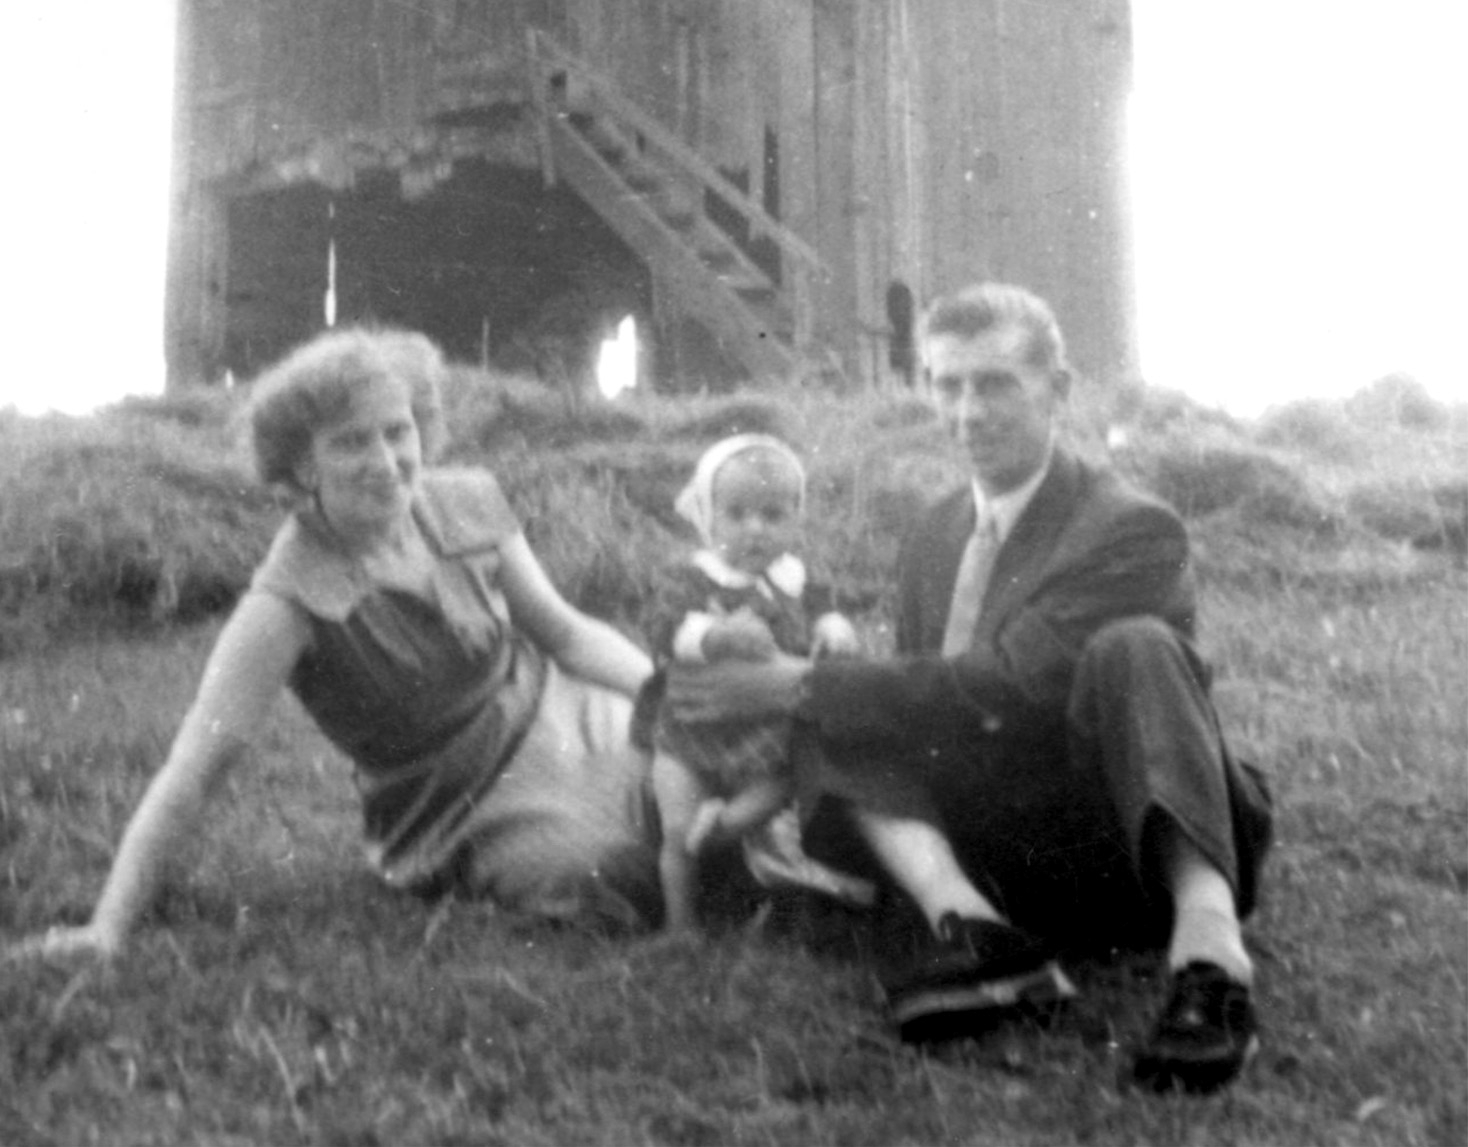
\includegraphics[width=0.65\textwidth]{photo/danuta_kufel.jpg}
\caption{Danuta Kufel z rodzicami.}
\end{center}
\end{figure}

\begin{figure}[!h]
\begin{center}
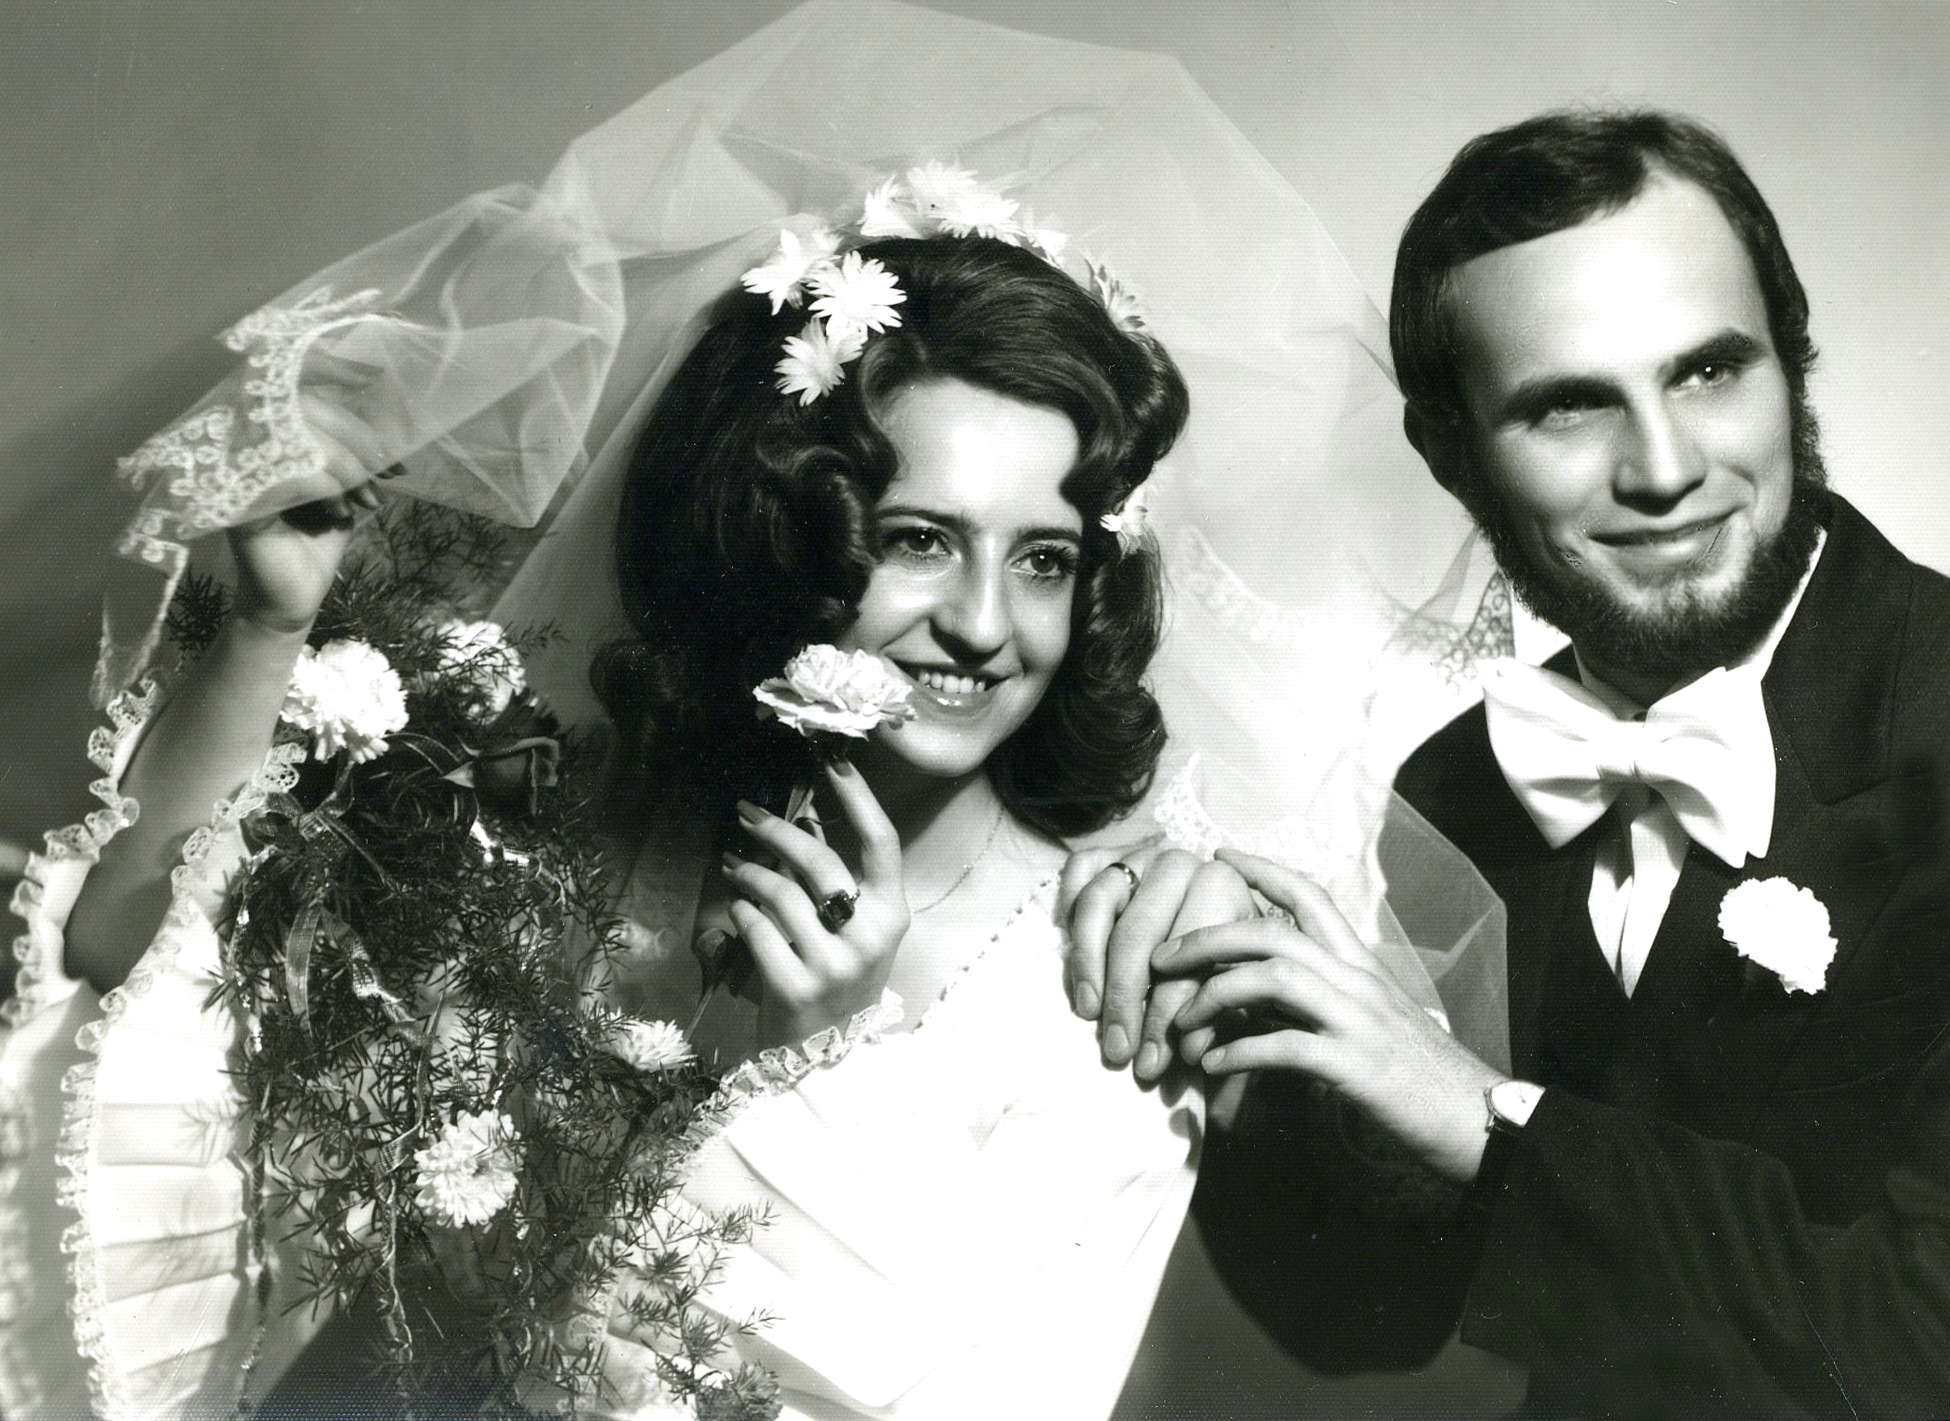
\includegraphics[width=0.65\textwidth]{photo/bogumil_danuta_lehman_slub.jpg}
\caption{Ślub Danuty Kufel i Bogumiła Lehmana}
\end{center}
\end{figure}

Doczekali się dwójki dzieci: \textbf{Michała, który przyszedł na świat 24 sierpnia 1978 r. oraz pierwszej córki u Lehmanów -- Kasi, która najbardziej uszczęśliwiła swym przybyciem dnia 18 lutego 1981 r. babkę Lehmankę.}

\begin{figure}[!h]
\begin{center}
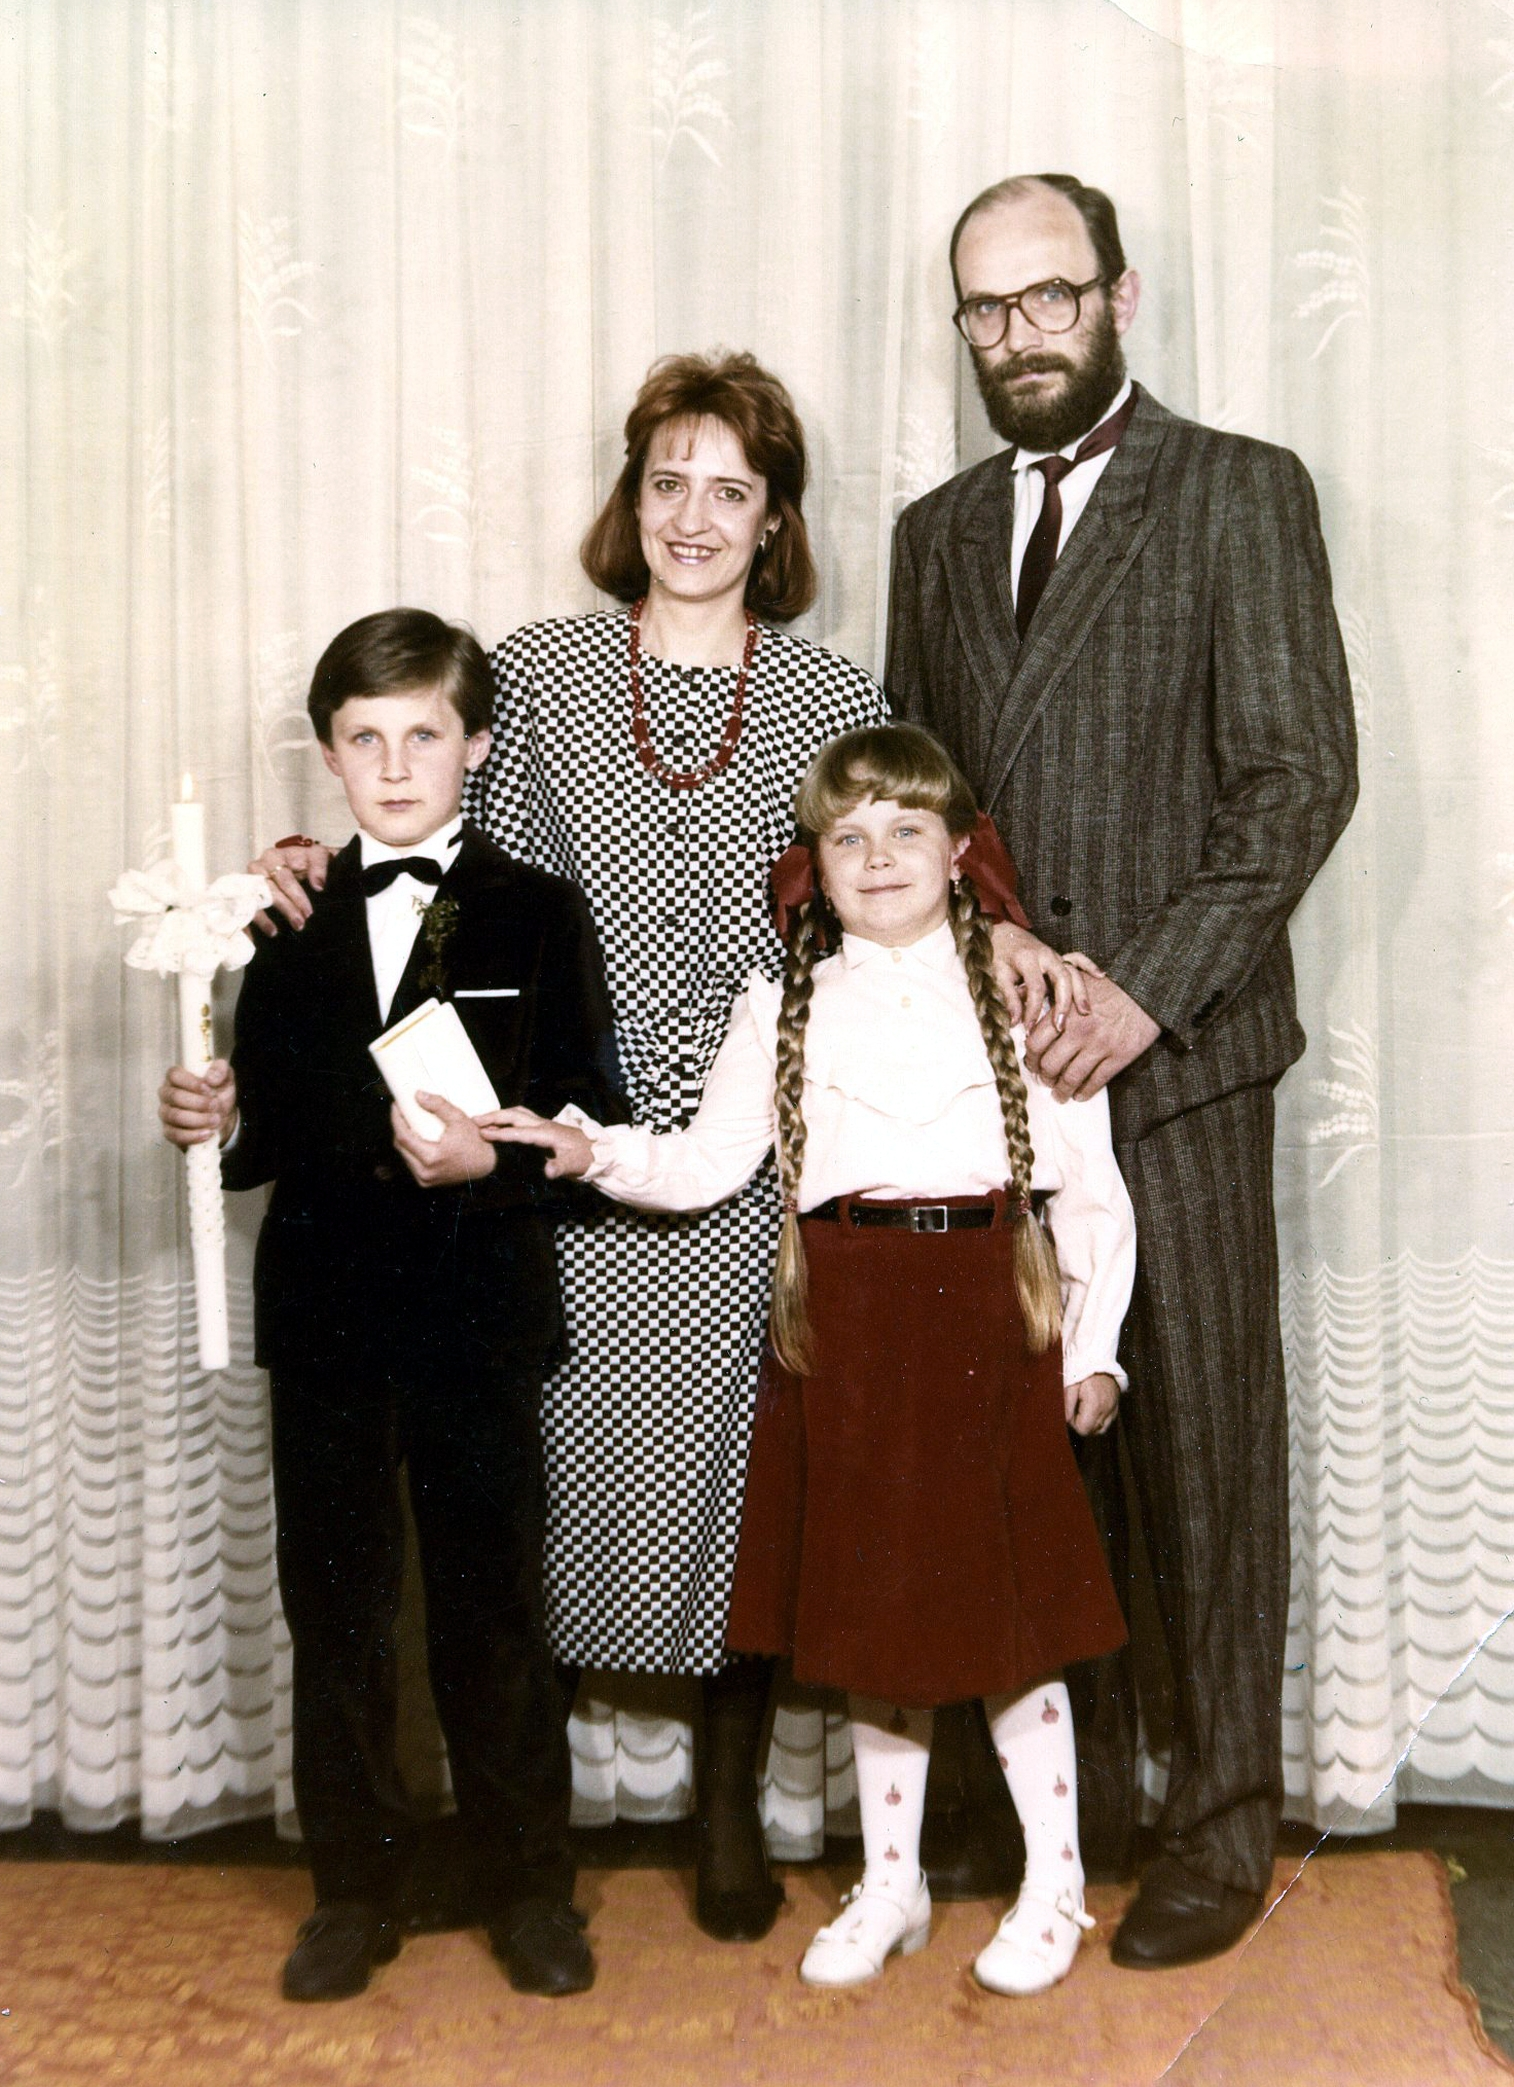
\includegraphics[width=0.32\textwidth]{photo/michal_lehman_komunia.jpg}
\caption[Pierwsza Komunia św. Michała Lehmana]{Pierwsza Komunia św. Michała Lehmana. Na zdj. z  siostrą Kasią i rodzicami.}
\end{center}
\end{figure}

\begin{figure}[!h]
\begin{center}
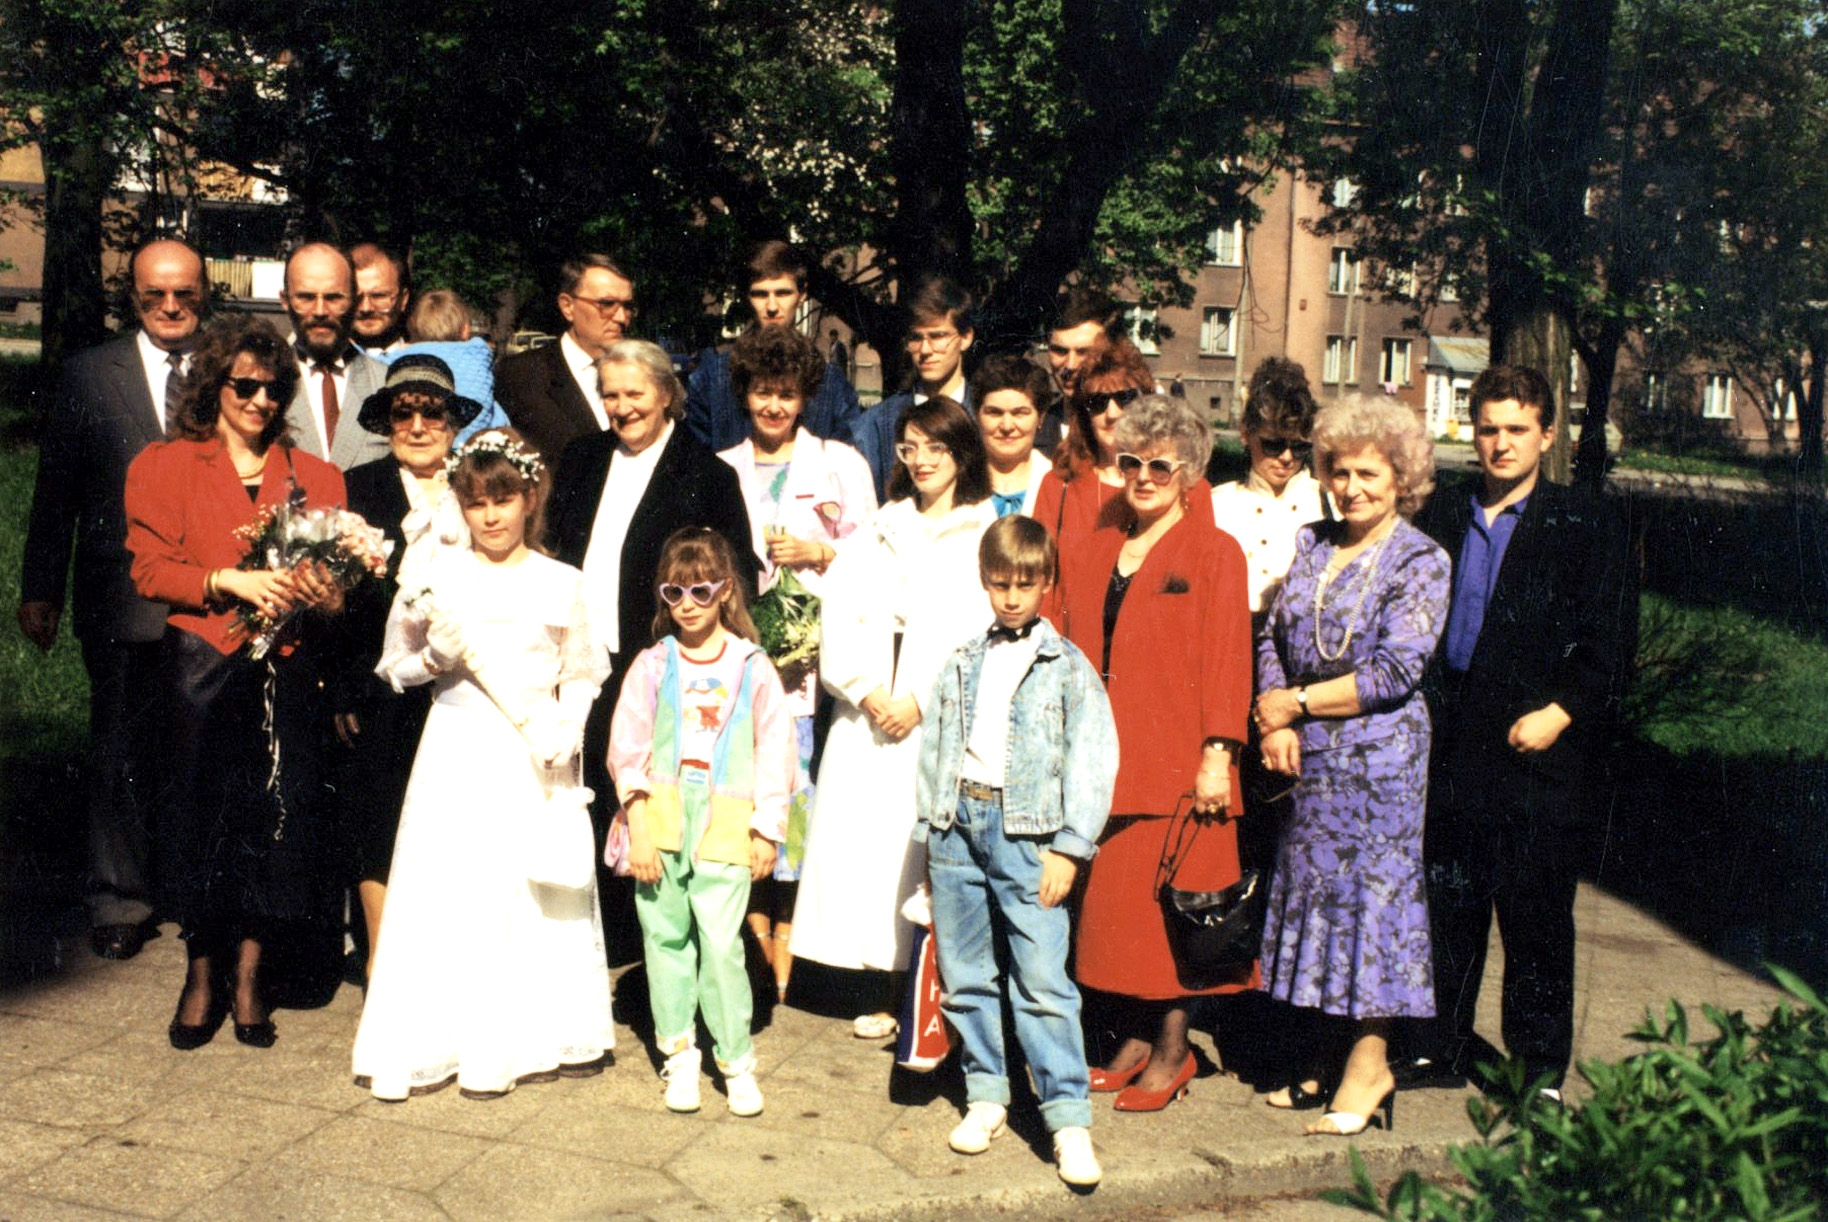
\includegraphics[width=0.7\textwidth]{photo/katarzyna_lehman_komunia.jpg}
\caption[Pierwsza Komunia św. Katarzyny Lehman]{Pierwsza Komunia św. Katarzyny Lehman. Na zdj. od lewej: Gustaw Lehman, przed nim Danuta Lehman (mama Kasi), obok jej Babka, za Danutą jej mąż Boguś, za nim Marek Lehman, obok niego Tadeusz Lehman, przed nim Irena Lehman (matka i babka Lehmanów), a przed nią Kasia Lehman, jej wnuczka. Obok babki Ireny stoi Marta Lehman (żona Gustawa), obok niej Małgosia Lehman (żona Marka), za nią Lubomira Lehman (żona Tadeusza),a za nią jej synowie: Tomasz, Krzysztof i Grzegorz, obok Lubomiry siostry bliźniaczki Danuty Lehman oraz ich matka Genowefa. }
\end{center}
\end{figure}

\begin{sidewaysfigure}
\begin{center}
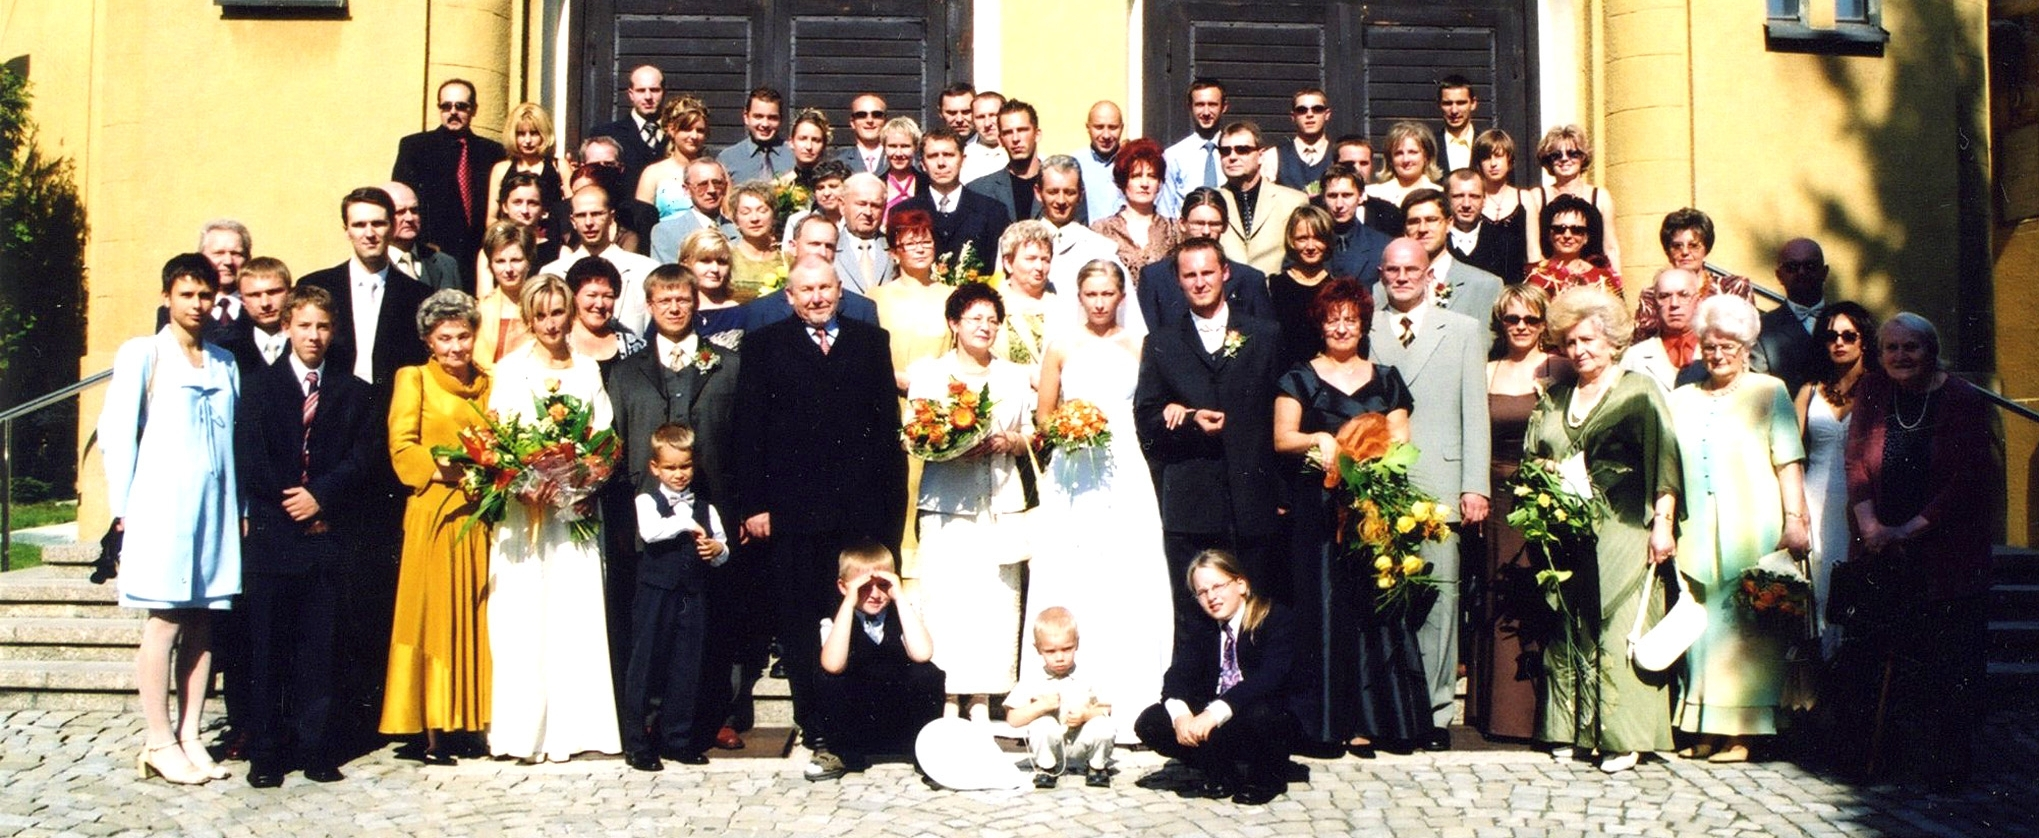
\includegraphics[width=240mm]{photo/michal_magdalena_lehman_slub.jpg}
\caption{Ślub Magdaleny Galińskiej i Michała Lehmana}
\end{center}
\end{sidewaysfigure}

Oboje ukończyli szkoły średnie i pracują; Michał w firmie ISTA w Katowicach, a Kasia w ,,Autopartnerze'' w~Tychach. \textbf{Michał dnia 20 września 2003 r. ożenił się z Magdaleną Galińską, córką Jana i Danuty z domu Danek urodzoną 6 stycznia 1977~r. w~Tychach.}

\begin{sidewaysfigure}
\begin{center}
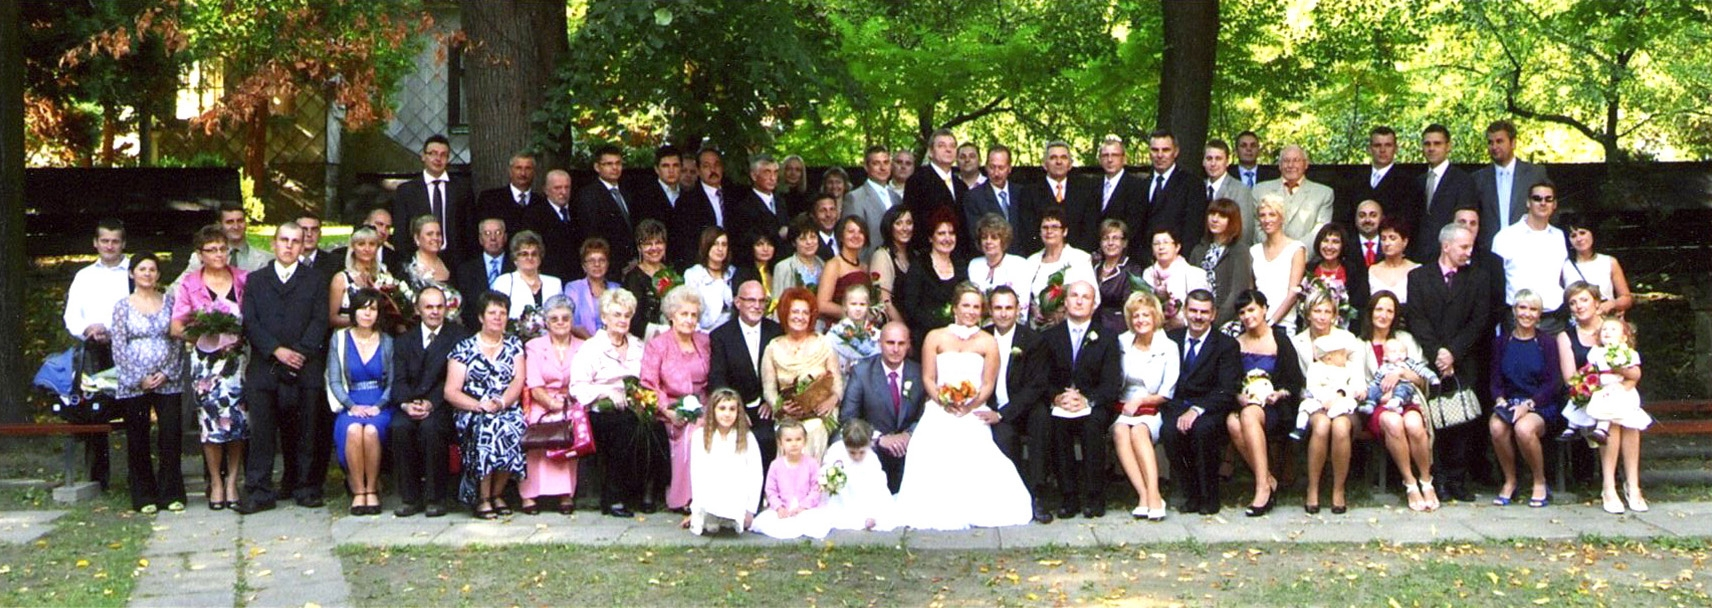
\includegraphics[width=240mm]{photo/katarzyna_robert_matlak_slub_2.jpg}
\caption{Ślub Katarzyny Lehman i Roberta Matlaka}
\end{center}
\end{sidewaysfigure}

\begin{figure}[!h]
\begin{center}
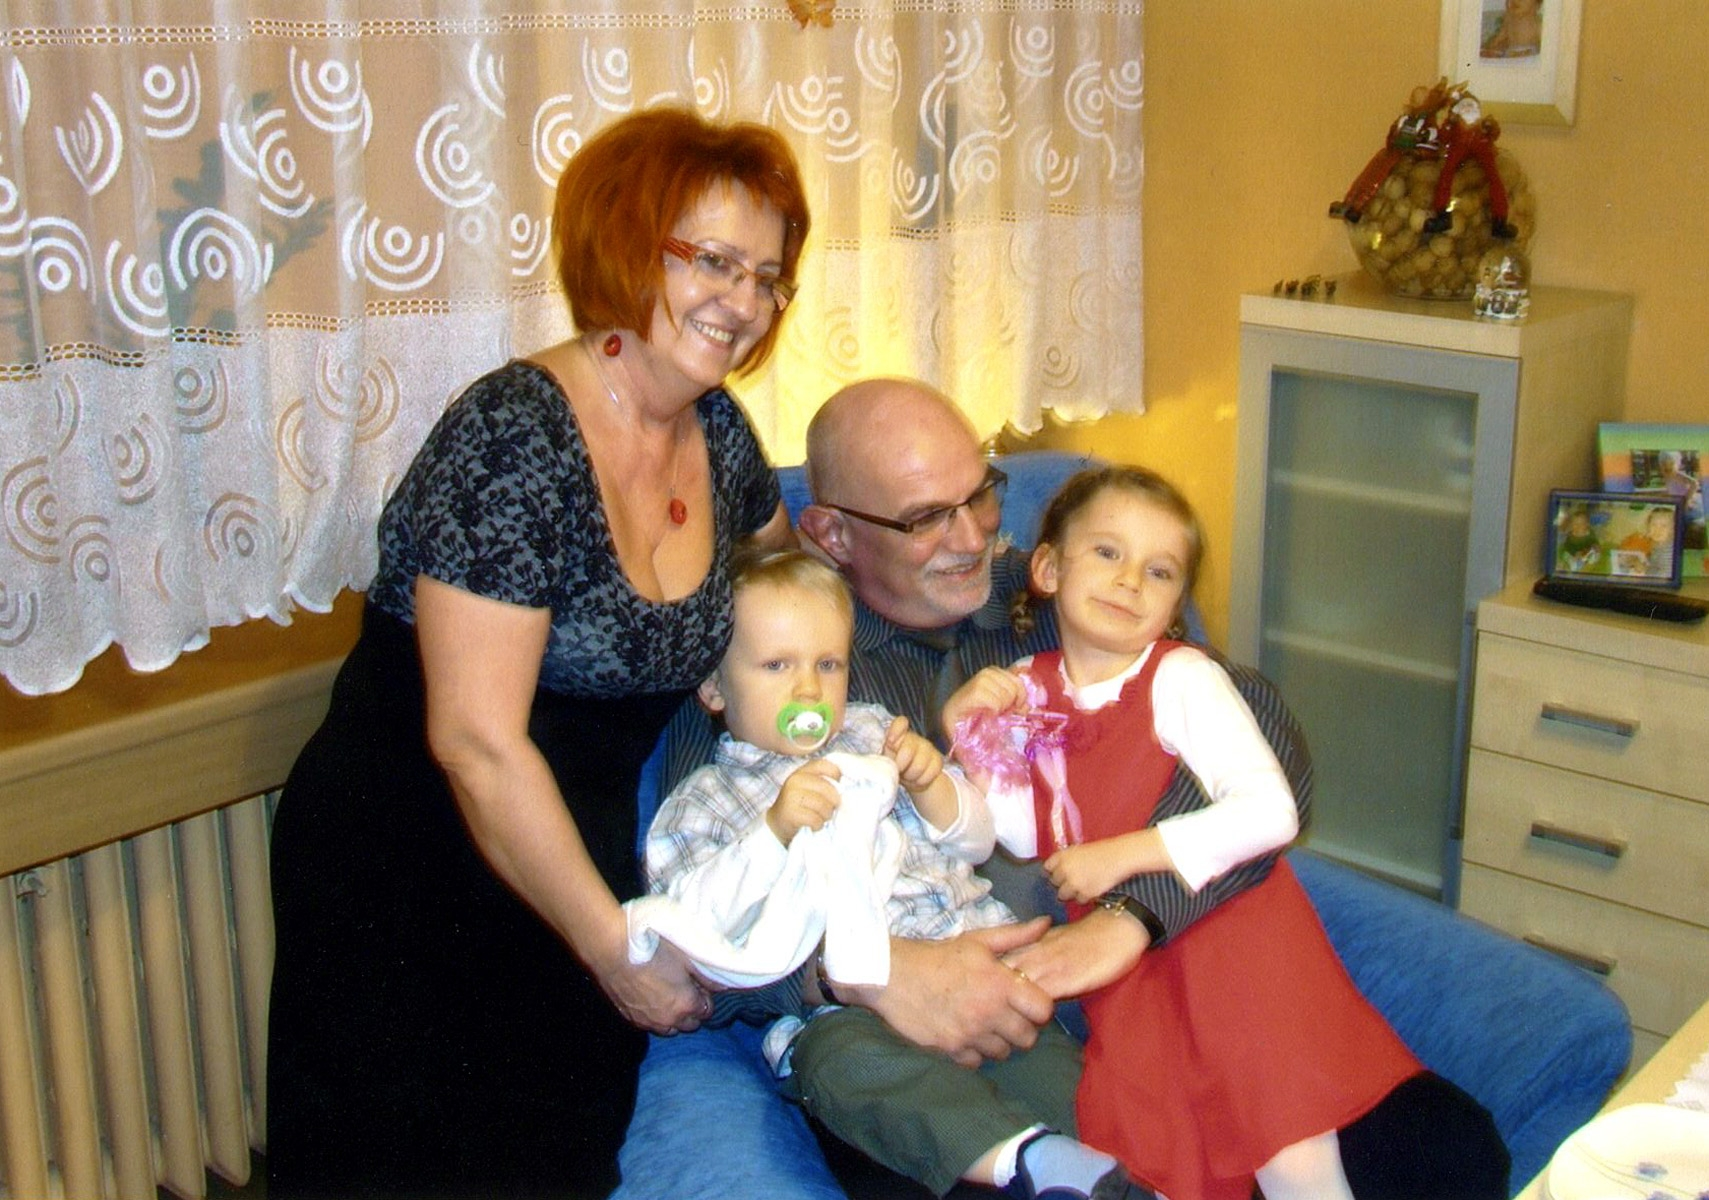
\includegraphics[width=0.5\textwidth]{photo/bogumil_danuta_lehman_z_wnukami.jpg}
\caption{Bogumił i Danuta Lehman z wnuczętami: Emilią i Antonim.}
\end{center}
\end{figure}



\newpage
Ukończyła studia na AWF i pracuje w szkole podstawowej w Tychach jako nauczycielka wychowania fizycznego. \textbf{Dnia 17 kwietnia2006 r. przyszła na świat w Mikołowie ich córka Emilia. a w dwa lata później Bogumił został dziadkiem, gdy przyszedł na świat w Mikołowie Antoni Lehman, prawnuk mojego stryja Antoniego.}

Kasia -- jedyna Lehmanka z urodzenia \textbf{wyszła za mąż za Roberta Matlaka ur. dnia 23 grudnia 1979 r. w~Tychach} z Eugeniusza i Doroty. \textbf{Pobrali się 19 września 2009 r. w~Szczyrku.}

Z ich związku przyszła szczęśliwie na świat \textbf{20 stycznia 2011 r. w Mikołowie ich pierwsza córka -- Zofia}.

\begin{figure}[!h]
\begin{center}
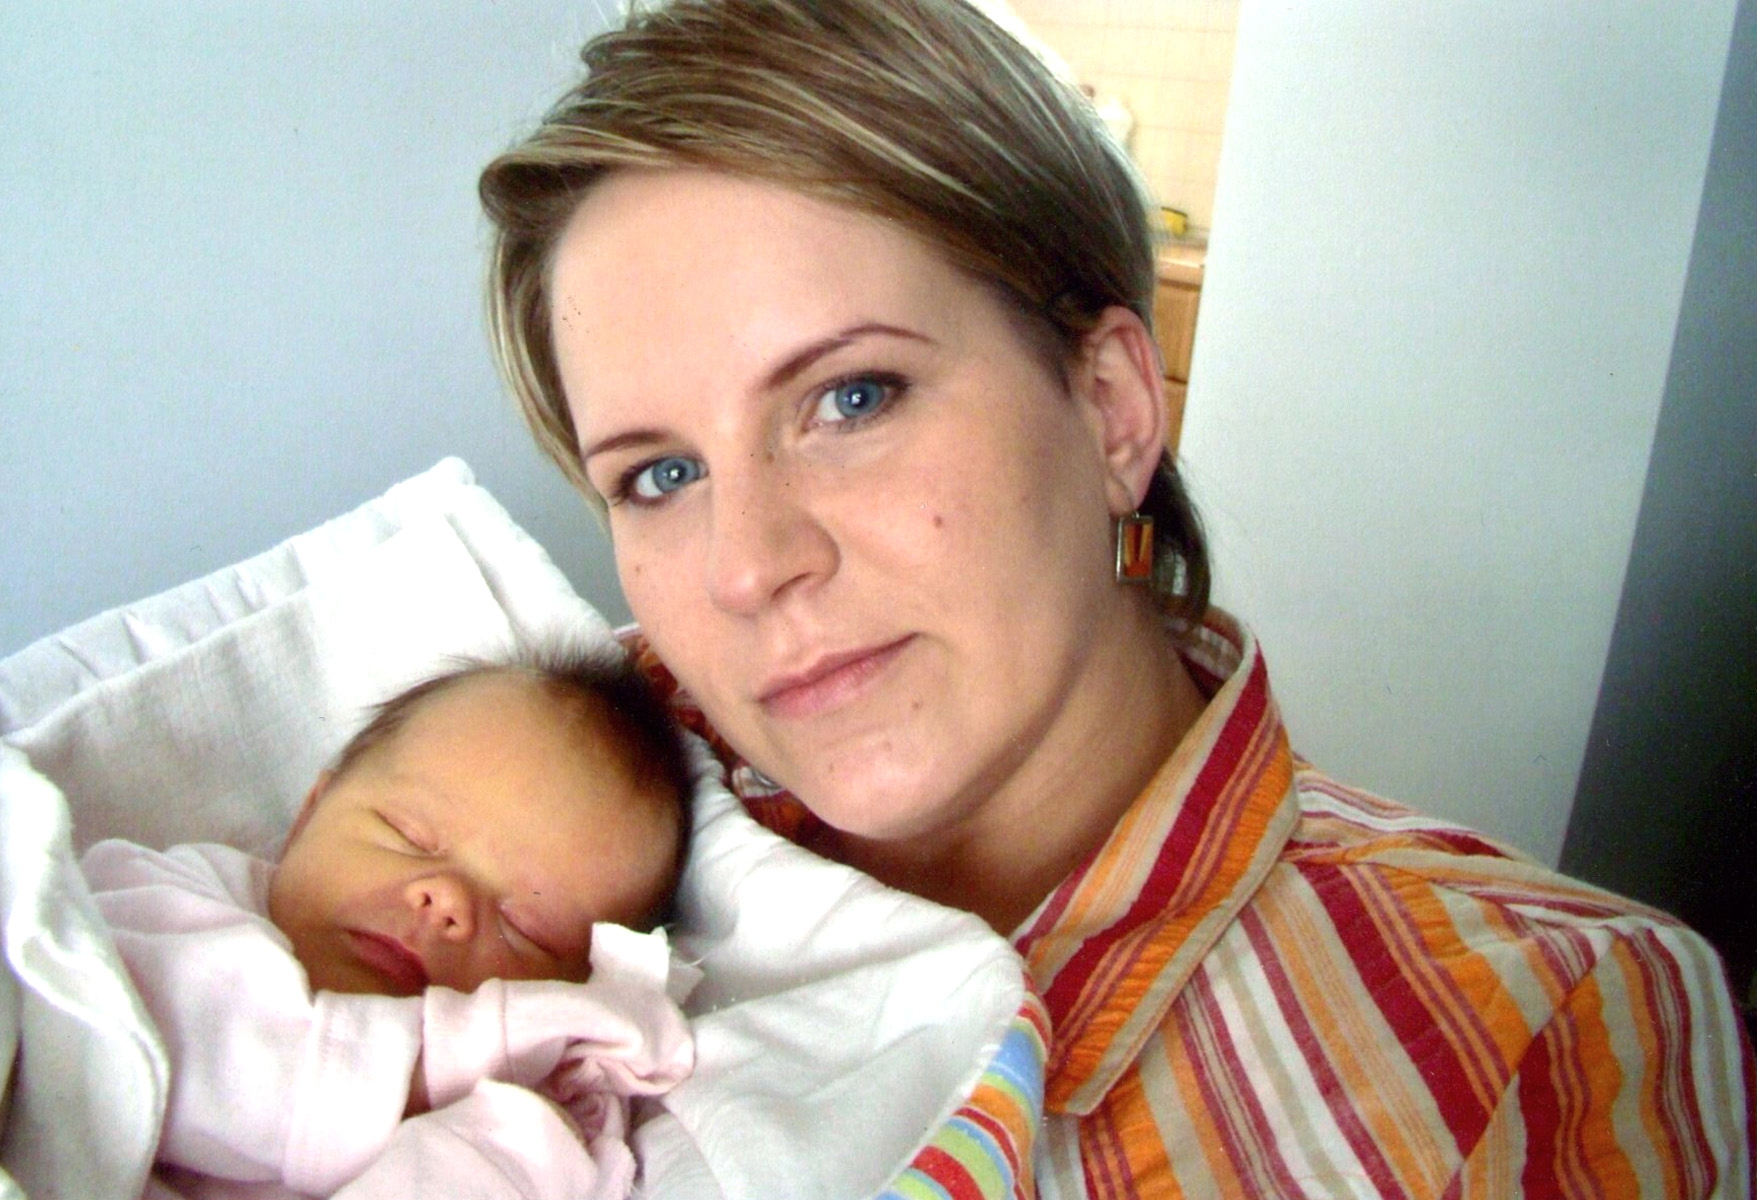
\includegraphics[width=0.6\textwidth]{photo/zofia_matlak.jpg}
\caption{Kasia Matlak z małą Zosią}
\end{center}
\end{figure}